% chktex-file 1
\documentclass[11pt,a4paper,openright,oneside]{book}
\usepackage{amsfonts, amsmath, amssymb,latexsym,amsthm, mathrsfs, enumerate}
\usepackage[catalan]{babel}
\usepackage{epsfig}
\usepackage{mathtools}
\usepackage{textcomp}
\usepackage{gensymb}
\usepackage[numbers]{natbib}
\usepackage{comment}
\usepackage{microtype}
\usepackage{multicol}
\usepackage{amsfonts}
\usepackage{bbm}
\usepackage{hyperref}
\usepackage{pgfplots}
\usepackage{dirtytalk}
\usepackage{tikz}
\usetikzlibrary{calc}
\usetikzlibrary{arrows}
\usepackage{wrapfig}
\usepackage{fancyhdr}



% \usepackage{parskip}
% \parskip=5pt
% \parindent=15pt
\usepackage[margin=1.2in]{geometry}
\usepackage{graphicx}
\usepackage{listings}
\usepackage[utf8]{inputenc}
\usepackage[T1]{fontenc}
\DeclarePairedDelimiter{\ceil}{\lceil}{\rceil}
\DeclarePairedDelimiter{\set}{\{}{\}}
\setcounter{page}{0}
\numberwithin{equation}{section}


\newtheorem{teo}{Teorema}[section]
\newtheorem*{teo*}{Teorema}
\newtheorem*{prop*}{Proposici\'o}
\newtheorem*{corol*}{Corol·lari}
\newtheorem{prop}[teo]{Proposici\'o}
\newtheorem{corol}[teo]{Corol·lari}
\newtheorem{lema}[teo]{Lema}
\newtheorem{defi}[teo]{Definici\'o}
\newtheorem{nota}{Notaci\'o}


\theoremstyle{definition}
\newtheorem{prob}[teo]{Problema}
\newtheorem*{sol}{Soluci\'o}
\newtheorem{ex}[teo]{Exemple}
\newtheorem{exs}[teo]{Exemples}
\newtheorem{obs}[teo]{Observaci\'o}
\newtheorem{obss}[teo]{Observacions}

\def\qed{\hfill $\square$}

\renewcommand{\refname}{Bibliografia}
% --------------------------------------------------
\usepackage{fancyhdr}

\lhead{}
\lfoot{}
\rhead{}
\cfoot{}
\rfoot{\thepage}

\pgfplotsset{compat=1.18}

% Add these accent definitions
\DeclareUnicodeCharacter{00ED}{\'i}
\DeclareUnicodeCharacter{00E9}{\'e}
\DeclareUnicodeCharacter{00E0}{\`a}
\DeclareUnicodeCharacter{00E8}{\`e}
\DeclareUnicodeCharacter{00F3}{\'o}
\DeclareUnicodeCharacter{00FA}{\'u}

\begin{document}



\thispagestyle{empty}

\begin{titlepage}
\begin{center}
\begin{figure}[htb]
\begin{center}
\includegraphics[width=6cm]{matematiquesinformatica-pos-rgb.png}
\end{center}
\end{figure}

\vspace*{1cm}
\textbf{\LARGE GRAU DE MATEM\`{A}TIQUES } \\
\vspace*{.5cm}
\textbf{\LARGE Treball final de grau} \\

\vspace*{1.5cm}
\rule{16cm}{0.1mm}\\
\begin{Huge}
\textbf{Encabiments Isomètrics\\ $C^1$ i $C^\infty$ en $\mathbb R^n$} \\
\end{Huge}
\rule{16cm}{0.1mm}\\

\vspace{1cm}

\begin{flushright}
\textbf{\LARGE Autor: Víctor Rubio Jiménez}

\vspace*{2cm}

\renewcommand{\arraystretch}{1.5}
\begin{tabular}{ll}
\textbf{\Large Director:} & \textbf{\Large Dr. Ignasi Mundet i Riera } \\
\textbf{\Large Realitzat a:} & \textbf{\Large  Departament de matemàtiques i informàtica   } \\
\\
\textbf{\Large Barcelona,} & \textbf{\Large \today }
\end{tabular}
\end{flushright}
\end{center}
\end{titlepage}


\newpage
\pagenumbering{roman} 
{\let\thefootnote\relax\footnote{2020 Mathematics Subject Classification. 53C42, 57R42, 53C21, 53C24, 53-02}} 
\section*{Abstract}
This work deals with isometric embeddings of riemannian manifolds in euclidean spaces, paying special attention to the flexibility obtained by relaxing the $C^\infty$ regularity condition to $C^1$. To this end, the proof of Nash's isometric embedding theorem is presented as it appears in \cite{nash1954}, stating that for any short $C^\infty$ embedding of an $n$-dimensional riemannian manifold in a euclidean space of dimension $n+k$, with $k \geq 2$, there exists a $C^1$ isometric embedding that is arbitrarily close to the original embedding. The improvement by \citet{kuiper1955}, which lowers the codimension to $k \geq 1$, is also presented.

To illustrate the rigidity of $C^\infty$ embeddings, this work demonstrates the classic result of the non-existence of $C^\infty$ isometric embeddings of flat tori in $\mathbb R^3$. Furthermore, drawing from \citet{schwartz2024}, we will derive the minimum aspect ratio required for a Möbius strip to admit a $C^\infty$ isometric embedding in 3-dimensional euclidean space. On the other hand, the flexibility of $C^1$ embeddings is showcased through the explicit construction of a $C^1$ isometric embedding of a flat torus in $\mathbb R^3$, following the work of \citet{borrelli2013}. This latter construction is directly related to the Nash-Kuiper theorem and employs convex integration methods.



\section*{Resum}
Aquest treball tracta sobre encabiments (\textit{embeddings}) isomètrics de varietats riemannianes en espais euclidians, parant especial atenció a la flexibilitat que s'obté en relaxar la condició de regularitat $C^\infty$ a $C^1$. Amb aquesta finalitat, es presenta la demostració del teorema d'encabiments isomètrics de Nash tal com apareix en \cite{nash1954}, que afirma que per a qualsevol encabiment $C^\infty$ curt d'una varietat riemanniana de dimensió $n$ en un espai euclidià de dimensió $n+k$, amb $k \geq 2$, existeix un encabiment isomètric $C^1$ arbitràriament proper a l'encabiment original. També es presenta la millora de \citet{kuiper1955} que baixa la codimensió a $k\ge1$. 

Per il·lustrar la rigidesa dels encabiments $C^\infty$, es demostra el resultat clàssic de la inexistència d'encabiments isomètrics $C^\infty$ en $\mathbb R^3$ d'un tor pla, i es demostra a partir de l'article de \citet{schwartz2024} una mida mínima per què una cinta de Möbius es pugui encabir isomètricament i $C^\infty$ en un espai euclidià de dimensió 3. Per l'altra banda, es mostra la flexibilitat dels encabiments $C^1$ amb la construcció explícita d'un encabiment isomètric $C^1$ d'un tor pla amb l'article de \citet{borrelli2013}. Aquesta darrera construcció és directament relacionada amb el teorema de Nash-Kuiper i utilitza mètodes d'integració convexa.

\newpage 


\section*{Agra\"{\i}ments}
Vull agrair a totes les persones que han fet possible la realització d'aquest treball de final de grau.
Al meu tutor, Ignasi Mundet i Riera, pels suggeriments, les revisions i les correccions que m'ha fet al llarg de tot el procés de redacció d'aquest treball. També per totes les reunions i les converses que hem tingut aquest semestre.
Als meus pares, els millors que hauria pogut demanar, per donar-me suport en tot moment i fer-me la persona que soc.
Als meus amics de Matemàtiques i Física, per les hores i hores a les sales de Farmàcia i de Raval, i a l'Antonio, pels anys que porta plantat a la facultat.
A la Marina, pel seu amor.

\newpage

\tableofcontents

\newpage


\chapter{Introducci\'o}

La geometria diferencial és l'estudi de les varietats diferenciables, és a dir, de varietats topològiques amb estructures diferenciables que permeten realitzar-hi càlcul infinitesimal. Si aquestes varietats diferenciables són subconjunts d'espais mètrics, es poden estudiar les seves propietats geomètriques induïdes per la mètrica de l'espai ambient en què es troben, el que anomenem \textit{geometria extrínseca}. Ara bé, les varietats diferenciables es poden dotar de mètriques riemannianes intrínseques, que permeten mesurar distàncies i angles locals sense fer referència a cap espai ambient. Anomenem les varietats diferenciables amb mètriques riemannianes \textit{varietats riemannianes}.

Aquests dos punts de vista envers les varietats diferenciables, com espais en si mateixos i com subconjunts d'altres espais, donen lloc a moltes preguntes pel que fa a la seva relació. Una d'elles és si tota varietat diferenciable es pot encabir (en anglès, \textit{embed}) o immergir (en anglès, \textit{immerse}) en un espai euclidià de dimensió superior. Com veurem al capítol \ref{cap:intro}, el teorema de Whitney afirma que tota varietat diferenciable $n$-dimensional suau, és a dir, de classe $C^\infty$, es pot encabir amb regularitat $C^\infty$ en un espai euclidià de dimensió $2n$. Ara bé, si aquesta varietat diferenciable és riemanniana, el teorema de Whitney no ens assegura que la immersió o l'encabiment sigui isomètric. És a dir, la mètrica induïda per l'espai ambient sobre la imatge de la varietat riemanniana per aquesta aplicació no coincidirà, en general, amb la mètrica intrínseca de la varietat. 

Un dels resultats clàssics pel que fa a la relació entre les mètriques intrínseca i extrínseca és el teorema egregi de Gauss, que veurem al capítol \ref{cap:intro}, segons el qual la curvatura gaussiana d'una superfície regular en l'espai euclidià tridimensional és invariant per isometries i es pot determinar a partir de les propietats intrínseques de la superfície. En efecte, aquest teorema troba certes restriccions a l'hora d'encabir o immergir de manera isomètrica i $C^\infty$ una varietat riemanniana en $\mathbb R^3$. Un dels exemples més importants d'aquestes limitacions és el fet que qualsevol superfície regular compacta immergida en $\mathbb R^3$ ha de tenir algun punt el·líptic. Això implica, com veurem en aquest treball, que cap tor pla es pot encabir de manera isomètrica i $C^\infty$ en $\mathbb R^3$.

Janet i \citet{cartan1927} van obtenir alguns resultats primerencs en l'estudi dels encabiments isomètrics de classe $C^\infty$ en espais euclidians arbitraris, demostrant que en el cas de varietats analítiques es pot trobar un encabiment suau localment isomètric en espais de dimensió majors o iguals a la dimensió de Janet, $s_n = \frac{n(n+1)}{2}$. Aquest resultat es va estendre posteriorment per part de Gromov i \citet{rokhlin1970} a espais de dimensió $q\ge s_n+n$ en el cas de varietats $C^\infty$. Com veiem, els espais ambients que asseguren l'existència d'encabiments isomètrics suaus poden arribar a ser de dimensió molt més alta que els que apareixen al teorema de Whitney.

La impossibilitat de trobar un encabiment isomètric suau del tor pla en $\mathbb R^3$ és deguda, en última instància, al fet que el tor pla té curvatura gaussiana nul·la, de manera que no pot tenir cap punt el·líptic. Ara bé, la curvatura d'una superfície regular està íntimament relacionada amb les segones derivades de les corbes que es poden definir sobre la varietat riemanniana, de manera que no està ben definida sobre la imatge de l'encabiment o immersió si aquesta aplicació no és $C^2$. És possible trobar un encabiment isomètric del tor pla si relaxem la condició de regularitat a $C^1$?

L'any 1954, John Forbes Nash Jr. va publicar un article sorprenent en què demostrava que per qualsevol encabiment $C^\infty$ d'una varietat riemanniana estrictament curt, és a dir, tal que escurci localment les distàncies entre punts, es pot trobar un encabiment isomètric de classe $C^1$ arbitràriament proper, sempre que la codimensió de l'espai ambient sigui major o igual que 2. Per fer-ho, va dissenyar un mètode iteratiu en cada etapa del qual la imatge de l'encabiment és modificada amb una mena de moviment espiral. Després d'un nombre finit d'etapes, s'obté un nou encabiment curt $C^\infty$, però el procés convergeix en un encabiment isomètric de classe $C^1$, pel qual la curvatura extrínseca de la seva imatge no està ben definida. La demostració és constructiva, però el requeriment de dues direccions normals a la imatge de l'encabiment impossibilita la seva aplicació per superfícies encabides en l'espai euclidià tridimensional. Un any més tard, Nicolaas H. Kuiper va trobar un mètode similar al de Nash que rebaixa la codimensió de l'espai ambient a $1$. La seva modificació del mètode de Nash substitueix el moviment espiral per una corrugació que només requereix l'existència d'una direcció normal a la imatge de l'encabiment.

Amb aquest rerefons, en aquesta memòria es treballarà des dels seus fonaments el problema dels encabiments isomètrics $C^1$ i $C^\infty$ de varietats riemannianes en espais euclidians, parant especial atenció a dos casos concrets de superfícies encabides en $\mathbb R^3$ per a les quals hi ha hagut desenvolupaments recents. En concret, estudiarem les cintes de Möbius planes rectangulars i els tors plans. Les cintes de Möbius planes rectangulars són aquelles obtingudes identificant dos costats d'un rectangle euclidià. Anomenem \textit{raó d'aspecte} la raó entre la longitud del costat més llarg i el costat més curt d'aquesta cinta. Demostrarem que és necessària una raó d'aspecte $\lambda>\sqrt3$ per tal que existeixi un encabiment isomètric suau en $\mathbb R^3$. 
Veurem també que, si es relaxa la condició de regularitat, és possible trobar un encabiment isomètric per a qualsevol cinta de Möbius en $\mathbb R^3$. En concret, es pot construir una aplicació contínua que sigui un encabiment $C^\infty$ a trossos. Pel que fa als tors plans, veurem la demostració que no existeix cap encabiment isomètric $C^\infty$ d'aquests en $\mathbb R^3$. Després de demostrar el teorema de Nash d'encabiments isomètrics $C^1$, veurem una aplicació de les tècniques que hi desenvolupa per trobar un encabiment isomètric d'un tor pla en $\mathbb R^3$.

\subsection*{Objectius del treball}
\begin{itemize}
    \item Donar una introducció a la geometria diferencial i a la geometria Riemanniana, amb especial atenció als encabiments isomètrics i a la regularitat de les aplicacions que els defineixen.
    \item Demostrar la impossibilitat d'encabir isomètricament el tor pla en $\mathbb R^3$ de manera suau.
    \item Demostrar el resultat recent de \citet{schwartz2024} que troba una raó d'aspecte mínima per encabir una cinta de Möbius isomètricament en $\mathbb R^3$ amb regularitat $C^\infty$, i mostrar que no existeix aquesta raó d'aspecte mínima si es relaxa la condició de regularitat de manera adequada.
    \item Enunciar i demostrar els teoremes de Nash d'immersions i encabiments $C^1$, i explicar el refinament de Kuiper.
    \item Mostrar el mètode de \citet{borrelli2013} per encabir de manera isomètrica $C^1$ el tor pla en $\mathbb R^3$, directament relacionat amb el teorema de Nash-Kuiper. 
\end{itemize}

\subsection*{Estructura de la mem\`oria}
El treball es divideix en cinc capítols, relacionats amb els objectius exposats a l'apartat anterior. El primer d'ells és aquesta mateixa introducció. El capítol 2 comença amb un breu recordatori de la definició de les classes de regularitat de funcions, per després centrar-se en la geometria diferencial i Riemanniana. Hi definim els conceptes necessaris per a la resta del treball, enunciant i demostrant els resultats més importants. També hi enunciem alguns teoremes importants, com el teorema de Sard i el teorema egregi de Gauss, sense donar-ne la demostració. Al final del capítol discutim la impossibilitat d'encabir isomètricament el tor pla en $\mathbb R^3$. El capítol 3 segueix la demostració completa d'un dels dos teoremes demostrats recentment sobre la cinta de Möbius \cite{schwartz2024}, enunciant també l'altre resultat. A més, expliquem una aplicació contínua que és un encabiment $C^\infty$ a trossos per la qual no hi ha raó d'aspecte mínima. El capítol 4 segueix l'article original de Nash en què demostra els seus teoremes sobre encabiments i immersions $C^1$. Algunes de les demostracions d'aquest capítol s'han reestructurat i fet més explícites que a l'article original. Acabem aquest capítol explicant el punt clau del refinament de Kuiper. Finalment, al capítol 5 exposem el treball de \citet{borrelli2013} per trobar un encabiment isomètric $C^1$ del tor pla en $\mathbb R^3$, sense donar massa detalls en les demostracions. 
\subsection*{Glossari de termes traduits al català}
Totes les fonts utilitzades en la redacció d'aquesta memòria són en anglès, de manera que ha calgut traduir alguns termes tècnics. Si bé la majoria d'aquests tenen traducció estàndard al català, alguns d'ells no en tenen. El cas més important per aquest treball és el del terme \textit{embedding}, que sovint s'escriu en anglès i en cursiva, però aquí apareixerà com \textit{encabiment}. A continuació introduïm un petit glossari d'alguns termes anglesos i la traducció per la qual hem optat en aquest treball. 

\begin{center}
    \begin{tabular}{ll}
    \hline
    \textbf{Terme anglès} & \textbf{Traducció al català} \\
    \hline
    \textit{Aspect ratio} & \textit{Raó d'aspecte} \\
    \textit{Bend} & \textit{Plec} \\
    \textit{Bump function} & \textit{Funció de relleu} \\
    \textit{Embedding} & \textit{Encabiment} \\
    \textit{Exhaustion function} & \textit{Funció d'exhauriment} \\
    \textit{Flatness} & \textit{Planor} \\
    \textit{Isometric default} & \textit{Defecte isomètric} \\
    \textit{Loops} & \textit{Voltes} \\
    \textit{Pre-bend} & \textit{Pre-plec} \\
    \textit{Smooth} & \textit{Suau} \\
    \textit{Stage} & \textit{Etapa} \\
    % \textit{Step} & \textit{Pas} \\
    \textit{Strain} & \textit{Corrugació} \\
    \hline
    \end{tabular}
\end{center}
\newpage
\pagenumbering{arabic}
\setcounter{page}{1}

\chapter{Introducció a la geometria diferencial}\label{cap:intro}

% {\color{red} El que haurem de fer per a que tot tingui sentit un cop estigui acabat és assegurar-nos que anomenem $x$ a les coordenades normals i $z$ a les coordenades de la carta. DE FET EL QUE TENIM AL CAPíTOL DE NASH ÉS $z$ per l'espai ambient i $x$ per la varietat.}

% {\color{red} ÉS MOLT IMPORTANT QUE DESPRÉS MIREM LA PÀGINA 24 DEL LEE, ON DEFINEIX TAMBÉ VARIETATS AMB FRONTERA}

\section{Introducció al capítol}
L'objectiu d'aquest capítol serà oferir els fonaments matemàtics necessaris per a entendre i justificar els resultats que es mostraran en els capítols posteriors, alhora que volem motivar l'interès d'aquests. Així, es definiran els conceptes i objectes matemàtics bàsics amb els quals treballarem, veurem algunes de les seves propietats i enunciarem i demostrarem alguns teoremes que seran clau en el treball que segueix.

Voldrem estudiar, al llarg d'aquest capítol, els conceptes de varietat topològica, varietat diferenciable i varietat Riemanniana. A un nivell intuïtiu, es tractarà d'espais topològics que es poden veure localment com espais reals $\mathbb R^n$, sobre els quals es pot fer càlcul infinitesimal i que es poden dotar de diferents mètriques. Prendrem especial atenció a la manera en què aquests espais es poden encabir (en anglès, \textit{embed}) en altres varietats i espais ambients. Si bé és generalment fàcil entendre i visualitzar aquests espais quan es consideren encabits en un espai $\mathbb R^n$, com el cas de les superfícies regulars en $\mathbb R^3$, cal notar que les varietats topològiques no requereixen aquest espai ambient per a la seva definició i estudi, sinó que en són independents. Aquest fet és molt rellevant, tot i que no el veurem aquí, en una de les aplicacions més interessants de la geometria diferencial, la teoria de la relativitat general, on l'espai-temps es modela com una varietat diferenciable de dimensió 4 i on no hi ha motiu per introduir cap espai ambient en el sentit clàssic.

Si bé seguirem la línia general d'estudi en molts llibres de referència, centrant-nos en funcions i aplicacions de regularitat $C^\infty$, més endavant ens caldrà treballar amb regularitats més baixes. Per aquest motiu, del primer que ens ocuparem serà de definir les funcions i aplicacions de classe $C^k$ i les normes associades. Això serà rellevant pel fet que també es pot definir la classe de regularitat d'una varietat diferenciable en un punt, i direm que una varietat és suau (en anglès, \textit{smooth}) quan és de classe $C^\infty$. La noció de suavitat no pot ser una propietat purament topològica, ja que no és preservada per homeomorfismes. L'exemple més evident és el d'un cercle i un quadrat, que són homeomorfs en $\mathbb R^2$, però el cercle és suau mentre que el quadrat no ho és. 

La suavitat de les varietats diferenciables serà clau per a desenvolupar eines potents en geometria diferencial, com veurem amb l'existència de particions de la unitat i el teorema de Whitney. Ara bé, veurem que això comporta un grau afegit de rigidesa en les propietats de les varietats Riemannianes pel que fa a la seva relació amb els encabiments (en anglès, \textit{embeddings}). L'última part d'aquest capítol serà dedicada a un exemple d'això mateix: demostrar que no existeix cap encabiment  $C^\infty$ del tor pla en $\mathbb R^3$ tal que preservi les distàncies entre els seus punts. Veurem, de fet, que el motiu principal d'aquesta impossibilitat es relaciona amb el concepte de curvatura gaussiana, que només es pot definir per a superfícies immerses en $\mathbb R^3$ de regularitat $C^2$ o superior. 

Les cites principals en aquest capítol seran \cite{lee2013} i \cite{warner1983}, pel que fa a varietats suaus, i \cite{chavel2006}, pel que fa a varietats Riemannianes.

\section{Classes de regularitat}
Comencem amb la definició estàndard de classes de regularitat de funcions i aplicacions.
\begin{defi}
    Siguin $U\subseteq\mathbb R^n$ un conjunt obert i $f:U\to\mathbb R$ una funció real contínua.
    Diem que $f$ és \textbf{ $k$-vegades derivable contínuament}, o \textbf{de classe $C^k(U)$}, amb $k\in\mathbb N_0$, si totes les derivades parcials d'ordre $k$, \begin{equation*}
        \frac{\partial^k f}{\partial (x^1)^{\alpha_1}\cdots\partial (x^n)^{\alpha_n}}\quad\text{tal que }\sum_{i=1}^n\alpha_i = k,
    \end{equation*} existeixen i són contínues en $U$.

    Si $g:U\to\mathbb R^m$ és una aplicació contínua, diem que $g$ és \textbf{ $k$-vegades derivable contínuament}, o \textbf{de classe $C^k(U)$}, si totes les seves components $g_i:U\to\mathbb R$ són $k$-vegades derivables contínuament.
\end{defi}
\begin{nota}
    No indicarem el domini en què una aplicació és de classe $C^k$ quan el domini sigui clar pel context.
\end{nota}

\begin{obss}
\end{obss}
\begin{itemize}
    \item Una aplicació $f$ és $0$ vegades derivable contínuament si i només si $f$ és contínua. 
    \item Si $f$ és $k$ vegades derivable contínuament, aleshores també és $j$ vegades derivable contínuament per $0\le j\le k$.
\end{itemize}

\begin{defi}
    Direm que una aplicació és \textbf{suau} o \textbf{de classe $C^\infty$} si és infinitament derivable, és a dir, si és $k$-vegades derivable contínuament per a tot $k\in\mathbb N_0$.
\end{defi}

\begin{defi}
    
    Siguin $U\subseteq \mathbb R^n$ un obert i $f:U\to\mathbb R$ una funció de classe $C^k(U)$. Definim la \textbf{norma $\|\cdot\|_{C^k(U)}$} de $f$ com

    \begin{equation*}
        \|f\|_{C^k(U)} := \sum_{|\alpha| \leq k} \sup_{x\in U} \left| \partial^\alpha f(x) \right|.
    \end{equation*}
    on $\alpha = (\alpha_1, \dots, \alpha_n)$, $|\alpha| = \alpha_1 + \dots + \alpha_n$, i
    \[
    \partial^\alpha f(x) := \frac{\partial^{|\alpha|} f(x)}{\partial (x^1)^{\alpha_1}\cdots\partial (x^n)^{\alpha_n}}.
    \]

    Per una aplicació $g:U\to\mathbb{R}^m$ de classe $C^k(U)$, definim la \textbf{norma $\|\cdot\|_{C^k(U)}$} de $g$ com
    \begin{equation*}
        \|g\|_{C^k(U)} := \sum_{|\alpha| \leq k} \sup_{x\in U} \left\| \partial^\alpha g(x) \right\|.
    \end{equation*}    
\end{defi}

\section{Varietats topològiques i diferenciables}
\begin{defi} 
    Sigui $M$ un espai topològic. Diem que $M$ és una \textbf{varietat topològica de dimensió $n$} si es compleixen les propietats següents:
    \begin{itemize}
        \item $M$ és \underline{Hausdorff}, és a dir, si per a cada $p,q\in M$ amb $p\neq q$ existeixen entorns oberts $U\subseteq M$ i $V\subseteq M$ de $p$ i $q$ respectivament tals que $U\cap V = \emptyset$,
        \item $M$ verifica el \underline{segon axioma de numerabilitat}, és a dir, existeix una base numerable de la topologia de $M$,
        \item $M$ és \underline{localment homeomorf a $\mathbb R^n$}, és a dir, per a cada $p\in M$ existeix un entorn obert $U\subseteq M$ de $p$ que és homeomorf a un obert de $\mathbb R^n$.
    \end{itemize}
\end{defi}

Per tal de poder descriure localment els punts de les varietats i de poder operar amb ells, és necessari introduir el concepte de carta coordenada. 

\begin{defi}
    Sigui $M$ una varietat topològica de dimensió $n$. Diem que un parell $(U,\varphi)$ és una \textbf{carta coordenada} o un \textbf{sistema de coordenades de $M$} si $U$ és un obert de $M$ i $\varphi:U\to\hat U$ és un homeomorfisme amb un obert $\hat U\subseteq\mathbb R^n$. Anomenem $U$ el \textbf{domini de la carta} i $\varphi$ l'\textbf{aplicació coordenada}. Donat un punt $p\in U$, anomenem \textbf{coordenades de $p$} respecte de la carta $(U,\varphi)$ als components de $\varphi(p)$ en la base canònica de $\mathbb R^n$.
\end{defi}
\begin{nota}
    Sovint anomenarem carta coordenada o simplement carta a l'aplicació coordenada $\varphi$.
\end{nota}

\begin{obs}
    De la definició de carta coordenada, observem que no tota varietat topològica $M$ es pot descriure globalment amb una única carta coordenada. Per exemple, si $M$ és homeomorf al cercle $\mathbb S^1$ amb la topologia induïda per $\mathbb R^2$, no es pot trobar cap aplicació $\varphi:M\to\mathbb R$ que sigui un homeomorfisme amb un obert de $\mathbb R$, ja que $\mathbb S^1$ és compacte.
\end{obs}

\begin{defi}
    Sigui $M$ una varietat topològica de dimensió $n$. Anomenem \textbf{estructura diferenciable de classe $C^k$} en $M$ una col·lecció $\mathcal F:=\set{(U_\alpha,\varphi_\alpha)}$ de cartes coordenades de $M$ que compleixen les propietats següents:
    \begin{itemize}
        \item $\bigcup_{\alpha\in A} U_\alpha = M$,
        \item Si $U_\alpha\cap U_\beta\neq\emptyset$, aleshores $\varphi_\beta\circ\varphi_\alpha^{-1}$ és $C^k$.
        \item $\mathcal F$ és maximal respecte de la propietat anterior, és a dir, si $\mathcal G$ és una altra estructura diferenciable de classe $C^k$ en $M$ i $\mathcal F\subseteq\mathcal G$, aleshores $\mathcal F = \mathcal G$.
    \end{itemize}
\end{defi}

\begin{defi}
    Sigui $M$ una varietat topològica de dimensió $n$. Diem que $(M, \mathcal F)$ és una \textbf{varietat diferenciable de dimensió $n$ i classe $C^k$} si $\mathcal F$ és una estructura diferenciable de classe $C^k$ en $M$.
\end{defi}

\begin{nota}
    Sovint ens referirem a $M$ com a varietat diferenciable, sense especificar-ne l'estructura diferenciable. Diem que la varietat diferenciable és suau si és de classe $C^\infty$.
\end{nota}

\begin{defi}
    Sigui $M$ una varietat diferenciable suau, $U\subseteq M$ un obert i $f:U\to\mathbb R$ una funció real. Diem que $f$ és \textbf{de classe $C^k$ en $U$} si $f\circ\varphi^{-1}$ és de classe $C^k$ per tota aplicació coordenada $\varphi$ de $M$.

    Una aplicació $\psi:M\to N$ és de classe $C^k(M,N)$ si per qualsevol $p\in M$ existeixen cartes $(U,\phi)$ al voltant de $p$ i $(V,\xi)$ al voltant de $\psi(p)$ tals que $\xi\circ\psi\circ\phi^{-1}$ és de classe $C^k$.
\end{defi}

\begin{defi}
    Siguin $M$ i $N$ varietats diferenciables de classe $C^k$. Diem que una aplicació $\psi:M\to N$ és un \textbf{difeomorfisme de classe $C^k$} si és bijectiva, de classe $C^k(M,N)$ i la seva inversa és de classe $C^k(N,M)$.
\end{defi}

\subsection{Particions de la unitat}
A continuació veurem algunes propietats de les varietats diferenciables que es desprenen del fet que verifiquen el segon axioma de numerabilitat. En aquesta subsecció ens centrarem en varietats diferenciables suaus, per tal d'obtenir el potent teorema de l'existència de particions de la unitat, que serà una eina essencial pel capítol \ref{chap:capitol_nash}.

\begin{defi}
    Sigui $M$ una varietat diferenciable. Anomenem \textbf{recobriment de $W\subseteq M$} a una col·lecció $\set{U_\alpha}$ de subconjunts de $M$ tals que $W = \bigcup_{\alpha\in A} U_\alpha$. Diem que el recobriment és un \textbf{recobriment per oberts} si tots els $U_\alpha$ són oberts, i un \textbf{recobriment per tancats} si tots els $U_\alpha$ són tancats.

    Donat un recobriment $\set{U_\alpha}$ de $W\subseteq M$, diem que $\set{V_\beta}$ n'és un \textbf{refinament} si per tot $\beta$ existeix un $\alpha$ tal que $V_\beta\subseteq U_\alpha$ i $\bigcup_{\beta\in B} V_\beta = \bigcup_{\alpha\in A} U_\alpha$.

    Diem que un recobriment $\set{U_\alpha}$ de $W\subseteq M$ és \textbf{localment finit} si per a cada $p\in W$ existeix un entorn $V$ de $p$ en $M$ tal que $V\cap U_\alpha = \emptyset$ per a tot $\alpha$ excepte un nombre finit. 
    
    Diem que una varietat diferenciable és \textbf{paracompacta} si qualsevol recobriment per oberts té un refinament localment finit.
\end{defi}

\begin{defi}
    Sigui $M$ una varietat diferenciable suau. Una \textbf{partició de la unitat en $M$} és una col·lecció $\set{\varphi_i}_{i\in I}$ de funcions reals de classe $C^\infty(M)$ tals que:
    \begin{itemize}
        \item $0\leq\varphi_i(p)\leq 1$ per a tot $i\in I$ i $p\in M$,
        \item $\sum_{i\in I}\varphi_i(p) = 1$ per a tot $p\in M$,
        \item El conjunt de suports $\set{\text{supp}(\varphi_i)}$ és localment finit, on el \textbf{suport} d'una funció és l'adherència del conjunt de punts del seu domini on la funció no és $0$.
    \end{itemize}
    Diem que la partició de la unitat és \textbf{subordinada al recobriment} $\set{U_\alpha}$ si per a cada $i\in I$ existeix un $\alpha$ tal que $\text{supp}(\varphi_i)\subseteq U_\alpha$.
\end{defi}

\begin{lema}\label{lema:paracompact}
    Sigui $X$ un espai topològic localment compacte (és a dir, tal que tot punt de $X$ té un entorn compacte), Hausdorff i tal que verifica el segon axioma de numerabilitat. Aleshores $X$ és paracompacte, i cada recobriment per oberts de $X$ té un refinament numerable i localment finit per oberts d'adherència compacta.
\end{lema}
{\color{green!50!black} 
    \textit{Prova.} 
    Com $X$ verifica el segon axioma de numerabilitat, existeix una base numerable de la topologia de $X$. Com $X$ és localment compacte, podem prendre d'aquesta base numerable els conjunts amb adherència compacta, i pel fet que $X$ és Hausdorff, aquesta col·lecció de subconjunts serà una base en si mateixa. Sigui $\set{U_i}_{i\in I}$ aquesta base.

    Sigui $G_1 := U_1$, i suposem que hem definit un cert $G_k=U_1\cup\cdots\cup U_{j_k}$. Sigui $j_{k+1}$ l'enter més petit tal que sigui estrictament més gran que $j_k$ i tal que 
    \begin{equation*}
        \overline{G_k}\subseteq \bigcup_{i = 1}^{j_{k+1}} U_i,
    \end{equation*}
    i definim 
    \begin{equation*}
        G_{k+1} := G_k\cup U_{j_{k+1}}.
    \end{equation*}
    D'aquesta manera, obtenim inductivament una successió de conjunts oberts $G_k$ tals que per tot $k$ tenim que
    \begin{enumerate}
        \item $\overline{G_k}$ és compacte,
        \item $\overline{G_k}\subseteq G_{k+1}$,
        \item $X = \bigcup_{k\in\mathbb N} G_k$.
    \end{enumerate}
    Ara sigui $\set{U_\alpha:\alpha\in A}$ un recobriment per oberts qualsevol. El conjunt $\overline{G_{k+1}}\setminus G_{k-1}$ és compacte i contingut en l'obert $G_{k+1}\setminus \overline{G_{k-2}}$. Per tot $i\ge3$, podem escollir un subrecobriment finit del recobriment per oberts $U_\alpha\cap(G_{k+1}\setminus \overline{G_{k-2}})$ de $\overline{G_k}\setminus G_{k-1}$, i es pot escollir un subrecobriment finit del recobriment per oberts $U_\alpha\cap G_3$ del conjunt compacte $\overline{G_2}$. Aquesta nova col·lecció serà un refinament numerable i localment finit per oberts d'adherència compacta del recobriment $\set{U_\alpha}$, com volíem veure. \qed
}
\begin{lema}\label{lema:bump}
    Existeix una funció real no negativa $\varphi:\mathbb R^n\to\mathbb R$ de classe $C^\infty$ que és igual a 1 en $[-1,1]^n$ i $0$ en el complementari de $(-2,2)^n$.
\end{lema}

{\color{green!50!black} 
    \textit{Prova.} 
    Sigui
    \begin{equation*}
        f(t) = \begin{cases}
            e^{-1/t} & \text{si } t > 0, \\
            0 & \text{si } t\le 0.
        \end{cases}
    \end{equation*}
    Observem que $f$ és clarament $C^\infty$ en $t<0$ i $t>0$. En el punt $t=0$, tenim que
    \begin{equation*}
        \lim_{t\to0^+} f(t) = \lim_{t\to0^+} e^{-1/t} = \lim_{x\to\infty} \frac{1}{e^x} = 0,
    \end{equation*}
    de manera que $f$ és contínua a $t=0$. Per veure que totes les derivades de $f$ existeixen i són iguals a $0$ en $t=0$, podem veure que totes les derivades de $\phi(t) = e^{-1/t}$ són el producte de $\phi(t)$ per un polinomi de $1/t$. En efecte, si $\phi^{(n)}(t) = \phi(t)P_n(1/t)$, aleshores $\phi^{(n+1)}(t) = \frac{1}{t^2}(\phi(t)P_n(1/t) - \phi(t)P_n'(1/t)) := \phi(t)P_{n+1}(1/t)$, on $P_{n+1}(1/t)$ és un nou polinomi en $1/t$. Com $\phi(t)$ decreix exponencialment quan $t\to0^+$ i tots els polinomis $P_n(1/t)$ creixen polinomialment quan $t\to0^+$, tenim que totes les derivades de $f$ existeixen i són iguals a $0$ en $t=0$.

    Així, podem definir
    \begin{equation*}
        g(t) = \frac{f(t)}{f(t) + f(1-t)},
    \end{equation*}
    que és $C^\infty$ per ser una composició de funcions $C^\infty$, i on el denominador no s'anul·la mai. Observem que $g(t)$ val 1 per $t\ge1$ i 0 per $t\le0$.

    A continuació, definim la funció $h$ com
    \begin{equation*}
        h(t) = g(t+2)g(2-t),
    \end{equation*}
    que és $C^\infty$ per ser producte de funcions $C^\infty$. Observem que $h(t)$ és la funció que buscàvem pel cas $n=1$. Per $n$ arbitrari, definim 
    \begin{equation}\label{eq:phi}
        \varphi = (h\circ x_1)\cdots(h\circ x_n),
    \end{equation}
    que té exactament les propietats que volíem.
    \qed
}

\begin{teo}[\textbf{Existència de particions de la unitat}]

    Sigui $M$ una varietat diferenciable de classe $C^\infty$ i $\set{U_\alpha:\alpha\in A}$ un recobriment per oberts de $M$. Aleshores, existeix una partició de la unitat numerable $\set{\varphi_i:i\in I}$ subordinada al recobriment $\set{U_\alpha}$ amb suports $\set{\text{supp}\varphi_i}$ compactes. A més, si no exigim que els suports siguin compactes, existeix una partició de la unitat $\set{\varphi_\alpha}$ subordinada al recobriment $\set{U_\alpha}$ amb $\text{supp}\varphi_\alpha \subseteq U_\alpha$ per a tot $\alpha\in A$, amb com a molt un conjunt numerable dels $\varphi_\alpha$ no idènticament zero.
\end{teo}

{\color{green!50!black} 
    \textit{Prova.} 
    Sigui $\set{G_i}$ un recobriment com el definit a la demostració del lema \ref{lema:paracompact} i definim $G_0=\emptyset$. Per cada punt $p\in M$, sigui $i_p$ l'enter més gran tal que $p\in M\setminus \overline{G_{i_p}}$. Escollim un $\alpha_p$ tal que $p\in U_{\alpha_p}$ i sigui $(V,\tau)$ una carta coordenada centrada en $p$ (és a dir, tal que $\tau(p)=0$) i tal que $V\subseteq U_{\alpha_p}\cap(G_{i_p+2}\setminus \overline{G_{i_p}})$ i $[-2,2]^n\subseteq\tau(V)$.

    Definim 
    \begin{equation*}
        \psi_p = \begin{cases}
            \varphi\circ\tau & \text{a } V, \\
            0 & \text{fora de } V.
        \end{cases}
    \end{equation*}
    on $\varphi$ és tal com l'hem definit a l'equació \eqref{eq:phi}. Aleshores, $\psi_p$ és una funció de classe $C^\infty$ en $M$ que val $1$ en un entorn $W_p$ de $p$ i té suport compacte en $V\subseteq U_{\alpha_p}\cap(G_{i_p+2}\setminus \overline{G_{i_p}})$. Per cada $i\ge1$, escollim un nombre finit de punts $p\in M$ tals que els respectius $W_p$ siguin un recobriment de $\overline{G_i}\setminus G_{i-1}$. Podem escollir un ordre qualsevol per les funcions corresponents $\psi_p$ per obtenir una successió $\set{\psi_j}$, i els seus suports formen una col·lecció localment finita de subconjunts de $M$. Amb això veiem que la funció 
    \begin{equation*}
        \psi = \sum_{j=1}^\infty \psi_j
    \end{equation*}
    és positiva i de classe $C^\infty$ en $M$. Ara, per tot $i=1,2,\dots$ definim 
    \begin{equation*}
        \varphi_i = \frac{\psi_i}{\psi}.
    \end{equation*}
    Les funcions $\varphi_i$ formen una partició de la unitat subordinada al recobriment $\set{U_\alpha}$ amb suports compactes.

    Si definim $\varphi_\alpha$ tals que siguin idènticament zero si cap $\varphi_i$ té suport en $U_\alpha$, i en cas contrari que siguin la suma de totes les $\varphi_i$ que hi tenen suport, aleshores tenim que $\varphi_\alpha$ formen una partició de la unitat subordinada al recobriment $\set{U_\alpha}$ amb com a molt un conjunt numerable dels $\varphi_\alpha$ no idènticament zero.

    Veiem que el suport de cada $\varphi_\alpha$ és contingut en $U_\alpha$, ja que si $\mathcal A$ és una col·lecció localment finita de conjunts tancats, aleshores $\overline{\bigcup_{A\in \mathcal A} A} = \bigcup_{A\in \mathcal A} A$. Ara bé, observem que en aquest cas el suport de $\varphi_\alpha$ no és necessàriament compacte.
    \qed
}
\begin{corol}
    Sigui $G$ un obert d'una varietat diferenciable de classe $C^\infty$ i $A\subseteq G$ un subconjunt tancat. Aleshores, existeix una funció $\varphi:M\to\mathbb R$ de classe $C^\infty$ en $M$ tal que
    \begin{enumerate}
        \item $0\leq\varphi(p)\leq 1$ per a tot $p\in M$,
        \item $\varphi(p) = 1$ per a tot $p\in A$,
        \item $\text{supp}\varphi\subseteq G$.
    \end{enumerate}
\end{corol}
{
\color{green!50!black} \textit{Prova.} 
Existeix una partició de la unitat $\set{\varphi, \psi}$ subordinada al recobriment $\set{G, M\setminus A}$ de $M$ amb $\text{supp}\varphi\subseteq G$ i $\text{supp}\psi\subseteq M\setminus A$. $\varphi$ és, per tant, la funció desitjada. \qed
}

A continuació utilitzarem l'existència de particions de la unitat per a demostrar l'existència d'un tipus diferent de funcions, que utilitzarem per demostrar el teorema de Whitney.

\begin{defi}\label{def:funció_exhauriment}
    Sigui $M$ una varietat diferenciable. Una funció $f:M\to\mathbb R$ és una \textbf{funció d'exhauriment} si és contínua i per qualsevol $c\in\mathbb R$, la preimatge $f^{-1}(-\infty,c]$ és compacta.
\end{defi}

\begin{prop}
    Sigui $M$ una varietat diferenciable suau. Aleshores, existeix una funció d'exhauriment $f:M\to\mathbb R_+$ de classe $C^\infty$.
\end{prop}
{
    \color{green!50!black} \textit{Prova.} 
    Sigui $\set{V_j}_j$ un recobriment numerable per oberts de $M$ per oberts amb adherències compactes, i sigui $\set{\psi_j}_j$ una partició de la unitat suau subordinada a aquest recobriment. Definim la funció
    \begin{equation*}
        f(p) = \sum_{j=1}^\infty j\psi_j(p)
    \end{equation*}
    De la definició de partició de la unitat obtenim que $f$ és positiva, i com és una suma localment finita de funcions $C^\infty$, és de classe $C^\infty$.

    Cal veure que és, efectivament, una funció d'exhauriment. Sigui $c\in\mathbb R$ i $N>c$ un enter. Per $p\not\in\bigcup_{j=1}^N \overline{V_j}$, tenim que $\psi_j(p)=0$ per a tot $1\le j\le N$. Per tant,
    \begin{equation*}
        f(p) = \sum_{j=N+1}^N j\psi_j(p) \ge \sum_{j=N+1}^N N\psi_j(p) =N\sum_{j=1}^N\psi_j(p) = N>c.
    \end{equation*}
    Equivalentment, si $f(p)\le c$, aleshores $p\in\bigcup_{j=1}^N \overline{V_j}$. Per tant, $f^{-1}(-\infty,c]$ és un subconjunt tancat del conjunt compacte $\bigcup_{j=1}^N \overline{V_j}$, i per tant és compacte.
    \qed
}



\subsection{Vectors tangents}
Un vector en $\mathbb R^n$ es pot pensar com un operador lineal sobre funcions reals diferenciables. En concret, donada una funció $f$ diferenciable en un punt $p\in\mathbb R^n$, el vector $v$ assigna a $f$ un valor real que és la derivada direccional de $f$ en la direcció i sentit de $v$ a $p$,
\begin{equation*}
    v(f) = v_1\frac{\partial f}{\partial x^1}\Big|_p + \cdots + v_n\frac{\partial f}{\partial x^n}\Big|_p,
\end{equation*}
amb les propietats de linealitat esperades,
\begin{equation*}
    v(f+g) = v(f) + v(g), 
\end{equation*}
\begin{equation*}
    v(\lambda f) = \lambda v(f),
\end{equation*}
i la propietat de Leibniz,
\begin{equation*}
    v(fg) = v(f)g(p) + f(p)v(g)
\end{equation*}
per qualssevol $f,g\in C^\infty(\mathbb R^n)$ i $\lambda\in\mathbb R$.

És evident que volem un anàleg a aquesta definició que sigui útil en el context de varietats diferenciables, per tal d'aprofitar el fet que aquestes són espais localment similars a $\mathbb R^n$. 

\begin{defi}
    Sigui $p$ un punt d'una varietat diferenciable de dimensió $n$. Un \textbf{vector tangent} a $M$ en $p$ és una aplicació lineal $v_p:C^\infty(M)\to\mathbb R$ que compleix la propietat de linealitat,
    \begin{equation*}
        v_p(\lambda f+\mu g) = \lambda v_p(f) + \mu v_p(g), 
    \end{equation*}
    i la propietat de Leibniz,
    \begin{equation*}
        v_p(fg) = v_p(f)g(p) + f(p)v_p(g).
    \end{equation*}
    Per qualssevol $f,g\in C^\infty(M)$ i $\lambda,\mu\in\mathbb R$.
    Anomenem el conjunt de tots aquests vectors tangents l'\textbf{espai tangent} a $M$ en $p$ i el denotem per $T_pM$.
\end{defi}

En concret, podem construir els següents vectors tangents:
\begin{equation*}
    \frac{\partial}{\partial x^i}\Big|_p(f) := \frac{\partial(f\circ\varphi^{-1})}{\partial x^i}(\varphi(p)),
\end{equation*}
on $(x^1,\dots,x^n)$ són les coordenades canòniques de $\mathbb R^n$ i $(U,\varphi)$ una carta coordenada centrada en $p$. Es pot demostrar que aquests vectors tangents formen una base de $T_pM$, de manera que $T_pM$ un espai vectorial de dimensió $n$. Tractant-lo com a tal, podem definir el seu espai dual.

\begin{defi}
    Sigui $M$ una varietat diferenciable. Per cada punt $p\in M$, definim \textbf{l'espai cotangent} a $p$, $T^*_pM$, com l'espai vectorial dual de $T_pM$,
    \begin{equation*}
        T^*_pM = (T_pM)^*.
    \end{equation*}
\end{defi}






Una eina essencial per treballar amb vectors tangents serà el concepte de \textbf{diferencial} d'una aplicació diferenciable entre varietats.
\begin{defi}
    Siguin $M$ i $N$ varietats diferenciables de classe $C^k$, $F:M\to N$ una aplicació diferenciable de classe $C^l$, $l\le k$, i $p\in M$. Anomenem \textbf{diferencial de $F$ en $p$} l'aplicació
    \begin{equation*}
        dF_p:T_pM\to T_{F(p)}N
    \end{equation*}
    que assigna a cada vector tangent $v\in T_pM$ el vector tangent $dF_p(v)\in T_{F(p)}N$ que compleix
    \begin{equation*}
        dF_p(v)(f) = v(f\circ F),
    \end{equation*}
    per a tota $f\in C^\infty(N)$.
\end{defi}
\begin{defi}
    Diem que una aplicació $F$ és \textbf{no singular} en $p\in M$ si $dF_p$ no és singular, és a dir, si el seu nucli és $\set0$.
\end{defi}
Dualitzant l'aplicació que defineix el diferencial, podem definir el \textit{pullback} d'una funció diferenciable, que serà particularment important per a l'estudi de mètriques Riemannianes.
\begin{defi}
    Siguin $M$ i $N$ varietats diferenciables suaus, $F:M\to N$ una aplicació diferenciable i $p\in M$. Anomenem \textbf{\textit{pullback} puntual de $F$ en $p$} l'aplicació
    \begin{equation*}
        dF_p^*:T_{F(p)}^*N\to T^*_pM 
    \end{equation*}
    obtinguda dualitzant el diferencial $dF_p$.
\end{defi}
Observem que el \textit{pullback} puntual està caracteritzat per la propietat
\begin{equation*}
    dF_p^*(w)(v) = w(dF_p(v)),
\end{equation*}
per a tot $v\in T_pM$ i $w\in T^*_{F(p)}N$.
\begin{obs}
    Sovint anomenem \textit{pushforward} a l'aplicació $dF_p$. Mentre el \textit{pushforward} actua sobre camps vectorials, el \textit{pullback} actua sobre funcions i formes diferencials. En concret, com veurem més endavant, es fa servir per transportar mètriques de $N$ a $M$.
\end{obs}

Una altra eina que necessitarem per descriure la geometria local de les varietats diferenciables és el de \textbf{fibrat tangent}.
\begin{defi}
    Sigui $M$ una varietat diferenciable. El \textbf{fibrat tangent} de $M$ és la unió disjunta dels espais tangents de tots els punts de $M$, 
    \begin{equation*}
        TM = \bigcup_{p\in M} T_pM,
    \end{equation*}
    juntament amb la \textbf{projecció} $\pi:TM\to M$ que a cada vector tangent li assigna el punt de la varietat al qual és tangent,
    \begin{equation*}
        \pi(v) = p,
    \end{equation*}
    on $v\in T_pM$.
\end{defi}
De la mateixa manera, podem definir el \textbf{fibrat cotangent} de $M$ com la unió disjunta dels espais cotangents de tots els punts de $M$,
\begin{equation*}
    T^*M = \bigcup_{p\in M} T^*_pM,
\end{equation*}
junt amb la \textbf{projecció} $\pi:T^*M\to M$ que envia $w\in T^*_pM$ a $p\in M$.

Es pot demostrar, tot i que no ho farem aquí, que tant el fibrat tangent com el fibrat cotangent són varietats diferenciables de dimensió $2n$. La demostració és més tècnica i requereix un cert joc amb les cartes coordenades i les projeccions, però recau en última instància en el simple fet que el fibrat tangent, així com el cotangent, assigna a cada punt de la varietat de dimensió $n$ un espai vectorial de dimensió $n$.

\subsection{Camps vectorials}
\begin{defi}
    Sigui $M$ una varietat diferenciable suau, i $(a,b)$ un interval obert de $\mathbb R$. Una \textbf{corba suau} en $M$ és una aplicació diferenciable $\sigma:(a,b)\to M$. Si es pot estendre a un interval obert $(a-\epsilon,b+\epsilon)$ per algun $\epsilon>0$ escrivim també $\sigma:[a,b]\to M$. Definim el \textbf{vector tangent} a $\sigma$ en $t\in(a,b)$ com

    \begin{equation*}
        \dot{\sigma}_t = d\sigma\left(\frac{d}{dr}\Big|_{t}\right)\in T_{\sigma(t)}M
    \end{equation*}
\end{defi}

\begin{defi}
    Un \textbf{camp vectorial} $X$ \textbf{al llarg d'una corba} $\sigma:[a,b]\to M$ és una aplicació $X:[a,b]\to TM$ que \say{aixeca} $\sigma$, és a dir, tal que $\pi\circ X = \sigma$, on $\pi$ és la projecció del fibrat tangent tal com l'hem definit abans. 

    Un \textbf{camp vectorial} $X$ \textbf{en un conjunt obert} $U\subseteq M$ és una aplicació $X:U\to TM$ que \say{aixeca} $U$, és a dir, tal que $\pi\circ X = \text{id}_U$.
\end{defi}


\subsection{Subvarietats, immersions, encabiments i difeomorfismes}
A continuació, definirem alguns dels conceptes més importants per aquest treball, en particular el concepte d'encabiment. A més, demostrarem el teorema de Whitney, que afirma que tota varietat diferenciable suau $n$-dimensional admet un encabiment suau en un espai euclidià. 
\begin{defi}
    Sigui $\psi:M\to N$ una aplicació diferenciable amb regularitat $C^k$, $k\ge 1$.
    \begin{enumerate}
        \item Diem que $\psi$ és una \textbf{immersió} si $d\psi_p$ és no singular per a tot $p\in M$.
        \item Diem que $\psi$ és un \textbf{encabiment} si és una immersió injectiva i un homeomorfisme sobre la seva imatge.
        \item Diem que $\psi$ és un \textbf{difeomorfisme} $C^r$ si és una injectiva amb inversa diferenciable amb regularitat $C^r$, $r\le k$.
        \item El parell $(M, \psi)$ és una \textbf{subvarietat de $N$} si $\psi$ és una immersió injectiva, i és una \textbf{subvarietat encabida} si és un encabiment.
    \end{enumerate}
\end{defi}

Es pot demostrar la següent proposició:
\begin{prop}\label{prop:encabiment_immersio}
    Sigui $\psi:M\to N$ una immersió injectiva entre varietats $C^k$, amb $k\ge 1$. Si qualsevol de les següents condicions és certa, aleshores $\psi$ és un encabiment:
    \begin{enumerate}
        \item $M$ és compacta.
        \item $\psi$ és un aplicació pròpia, és a dir, la imatge inversa de qualsevol compacte de $N$ és compacta.
        \item $\psi$ és oberta o tancada.
    \end{enumerate}
\end{prop}

En parlar de subvarietats encabides en espais euclidians $\mathbb R^n$, també serà interessant parlar del que anomenarem \textbf{vectors normals}.
\begin{defi}\label{def:espai_normal}
    Sigui $M\subseteq\mathbb R^n$ una subvarietat $m$-dimensional encabida en $\mathbb R^n$. Per tot punt $x\in M$, definim l'\textbf{espai normal} a $M$ en $x$, $N_xM$, com el subespai vectorial de $T_x\mathbb R^n$ ortogonal a $T_xM$ pel producte escalar euclidià.
\end{defi}

Un dels tipus de subvarietats que més ens interessarà seran les subvarietats encabides en $\mathbb R^n$. En concret, posarem particular atenció a $n=3$.

\begin{defi}
    Diem que $S\subseteq\mathbb R^3$ és una \textbf{superfície regular (i simple)} si és la imatge d'un encabiment suau $\psi:T\to\mathbb R^3$ d'una regió elemental $T\subseteq\mathbb R^2$ en $\mathbb R^3$.
\end{defi}

\begin{ex}\label{ex:tor}
    Siguin $R>r>0$. Per $T = [0,1)\times[0,1)\subseteq\mathbb R^2$, sigui $\psi:T\to\mathbb R^3$ l'aplicació
    \begin{equation*}
        \psi(u,v) = \left( (R+r\cos(2\pi v))\cos(2\pi u), (R+r\cos(2\pi v))\sin(2\pi u), r\sin(2\pi v) \right).
    \end{equation*}
    Aleshores, $\psi$ és un encabiment suau i $S = \psi(T)$ és una superfície regular. Aquest és un dels possibles encabiments del \textbf{tor} en $\mathbb R^3$ com a superfície regular.
\end{ex}

\subsubsection{Els teoremes de Whitney}
La possibilitat de prendre varietats diferenciables arbitràries com a subvarietats d'altres espais amb estructura més senzilla, com és el cas de $\mathbb R^n$, pot oferir una major facilitat a l'hora de treballar amb aquestes varietats. Si bé, com hem dit més amunt i hem vist fins ara, les varietats diferenciables suaus no requereixen ser subvarietat de cap espai euclidià, sí és cert que totes elles poden ser subvarietats encabides de $\mathbb R^N$ per a $N$ prou gran.

El teorema de Whitney (o teoremes, degut a les seves diverses formulacions) afirma això mateix, que tota varietat diferenciable suau $n$-dimensional $M$ admet un encabiment suau en $\mathbb R^{2n+1}$. Per demostrar el teorema de Whitney, cal utilitzar el teorema de Sard. No demostrarem aquest darrer teorema, però el farem servir en la demostració del teorema de Whitney.
\begin{nota}
    Sempre que parlem d'encabiments o immersions de varietats en espais $\mathbb R^n$, suposarem que aquests tenen la mètrica euclidiana.
\end{nota}
\begin{defi}
    Sigui $F:M\to N$ una aplicació diferenciable. Diem que $p\in M$ és un \textbf{punt regular} de $F$ si $dF_p$ és exhaustiva. Altrament, diem que és un \textbf{punt crític}. Un punt $c\in N$ és un \textbf{valor regular} de $F$ si tots els punts de la preimatge $F^{-1}(c)$ són regulars.
\end{defi}

\begin{teo}[\textbf{Teorema de Sard}]
    Siguin $M, N$ varietats diferenciables suaus i $F:M\to N$ una aplicació de classe $C^\infty$. Aleshores, la imatge del conjunt de punts crítics és un subconjunt de mesura zero de $N$. En concret, si la dimensió de $M$ és menor que la de $N$, $F(M)$ té mesura zero en $N$.
\end{teo}

\begin{lema}
    Sigui $M\subseteq\mathbb R^N$ una subvarietat suau $n$-dimensional. Per tot $v\in \mathbb R^N\setminus R^{N-1}$, sigui $\pi_v : \mathbb R^N\setminus R^{N-1}\to S^{N-1}$ la projecció amb nucli $\mathbb Rv$, on identifiquem $\mathbb R^{N-1}$ amb el subespai de $\mathbb R^N$ amb la última coordenada nul·la. Si $N>2n+1$, aleshores hi ha un conjunt dens de vectors $v\in \mathbb R^N\setminus R^{N-1}$ tals que $\pi_v|_M$ és una immersió injectiva de $M$ en $\mathbb R^{N-1}$.
\end{lema}
{
    \color{green!50!black} 
    \textit{Prova.}
    Observem les següents equivalències entre propietats:
    \begin{itemize}
        \item $\pi_v|_M$ és injectiva $\iff$ $p-q$ mai és paral·lel a $v$ per a $p,q\in M$ diferents.
        \item $\pi_v|_M$ és una immersió suau $\iff$ $T_pM$ no conté vectors no nuls de $\ker d(\pi_v)_p$ per a $p\in M$.
    \end{itemize}
    Com $\pi_v$ és lineal, el seu diferencial és la mateixa aplicació lineal, de manera que aquesta última condició és equivalent a demanar que $T_pM$ no contingui vectors no nuls paral·lels a $v$.

    Siguin ara
    \begin{align*}
        \Delta_M &= \set{(p,p):p\in M}\subseteq M\times M,\\
        M_0 &= \set{(p,0):p\in M}\subseteq TM,\\
    \end{align*}
    i considerem les aplicacions següents cap a l'espai projectiu real $\mathbb {RP}^{N-1}$:
    \begin{align*}
        \kappa:(M\times M)\setminus\Delta_M&\to\mathbb {RP}^{N-1},\\
        (p,q) &\mapsto [p-q]\\
    \end{align*}
    i
    \begin{align*}
        \tau:(TM)\setminus M_0&\to\mathbb {RP}^{N-1},\\
        (p,w) &\mapsto [w]
    \end{align*}
    On $[v]$ denota la classe d'equivalència del vector $v$ de $\mathbb R^N\setminus\set0$ com a punt de $\mathbb {RP}^{N-1}$.

    Ambdues aplicacions són suaus, ja que són composició d'aplicacions suaus amb la projecció $\mathbb R^N\setminus\set0\to\mathbb {RP}^{N-1}$, i les dues condicions donades al principi de la demostració són equivalents a la condició que $[v]$ no sigui imatge de $\kappa$ ni de $\tau$. Com els dominis d'ambdues aplicacions tenen dimensió $2n<N-1$, pel teorema de Sard, les imatges de $\kappa$ i $\tau$ tenen mesura zero en $\mathbb {RP}^{N-1}$ i, per tant, el conjunt de vectors que pertanyen a les classes d'equivalència que no pertanyen a cap d'aquestes imatges és dens.
    \qed
}

Iterant el procés donat en aquesta demostració, veiem que podem reduir la dimensió de l'espai ambient d'un encabiment a partir d'una sèrie de projeccions sobre subespais d'una dimensió més baixa, fins arribar a un espai de dimensió $2n+1$. Tot i que això només ens ofereix una immersió i no un encabiment, és possible modificar lleugerament el lema per assegurar un encabiment. No detallem aquí de quina manera, però s'acaba reduint a imposar una condició no gaire restrictiva a l'elecció de $v$.

\begin{lema}\label{lema:encabiment_whitney}
    Sigui $M$ una varietat suau $n$-dimensional. Si $M$ admet un encabiment suau propi en algun espai $\mathbb R^N$, aleshores $M$ admet un encabiment suau propi en $\mathbb R^{2n+1}$.
\end{lema}

Al lema anterior, \textbf{propi} tan sols vol dir que l'encabiment és una aplicació pròpia, és a dir, tal que la preimatge de qualsevol compacte és compacta. Hem vist que podem reduir la dimensió de l'espai ambient en què haguem encabit la nostra varietat, però encara queda veure que es pot encabir en algun espai real per acabar la demostració.

\begin{teo}[\textbf{Teorema de Whitney}]\label{teo:whitney}
    Tota varietat diferenciable suau $n$-dimensional admet un encabiment suau en $\mathbb R^{2n+1}$.
\end{teo}
{
    \color{green!50!black} \textit{Prova.}
    Sigui $M$ una varietat diferenciable suau $n$-dimensional. Com hem dit, només cal veure que $M$ admet un encabiment en algun espai $\mathbb R^N$ amb $N$ prou gran.

    Suposem primer que $M$ és compacta. Aquest és el cas més senzill. Sigui $\set{B_1,\dots,B_m}$ un recobriment finit per boles coordenades, de manera que per cada $i$ existeix un domini de coordenades $B_i'\supseteq \overline{B_i}$ i una carta coordenada $\varphi_i:B_i'\to\mathbb R^n$ que és homeomorfisme de $\overline{B_i}$ amb un compacte de $\mathbb R^n$.

    Sigui $\set{\rho_i}_i$ un conjunt de funcions de relleu, tals que $\rho_i$ val 1 en $\overline{B_i}$ i 0 en $\mathbb R^n\setminus B_i'$. L'existència d'aquests conjunts de funcions de relleu és conseqüència de l'existència de funcions de relleu en espais euclidians, com hem vist al lema \ref{lema:bump}. Definim una aplicació suau

    \begin{align*}
        F:M&\to\mathbb R^{nm + m},\\
        p&\mapsto \left(\rho_1(p)\varphi_1(p),\dots,\rho_m(p)\varphi_m(p), \rho_1(p),\dots,\rho_m(p)\right)
    \end{align*}
    on $\rho_i\varphi_i$ és zero fora del suport de $\rho_i$. Com hem suposat que $M$ és compacte, només cal veure que $F$ és una immersió injectiva suau, per la proposició \ref{prop:encabiment_immersio}.

    Vegem que $F$ és injectiva. Suposem $F(p) = F(q)$ per a $p,q\in M$. Com els $B_i$ són un recobriment de $M$, existeix un $i$ tal que $p\in B_i'$, i $\rho_i(p)=1$. Com $F(p) = F(q)$, tenim que $\rho_i(p) = \rho_i(q)$ i $\rho_i\varphi_i(p) = \rho_i\varphi_i(q)$. Com $\rho_i(p)=1$, tenim que $\varphi_i(p) = \varphi_i(q)$. Com $\varphi_i$ és un homeomorfisme, tenim que $p=q$. Així, $F$ és injectiva.

    Vegem que $F$ és una immersió suau. Sigui $p\in M$ i $p\in B_i$. Com $\rho_i\equiv1$ en un entorn de $p$, tenim $d(\rho_i\varphi_i)_p = d\varphi_p$, que és injectiva. Per tant, $dF_p$ és injectiva, i $F$ és una immersió suau.
    Amb això acabem el cas de $M$ compacte.

    Suposem ara que $M$ no és compacte. Sigui $f:M\to \mathbb R$ una funció d'exhauriment suau, tal com les hem definit a la definició \ref{def:funció_exhauriment}. Pel teorema de Sard, per tot enter no negatiu $i$ existeixen valors regulars $a_i,b_i$ de $f$ tals que $i<a_i<b_i<i+1$. Definim els subconjunts de $M$
    \begin{align*}
        D_0 &= f^{-1}(-\infty,1],\quad E_0 = f^{-1}(-\infty,a_1],\\
        D_i &= f^{-1}(i,i+1],\quad E_i = f^{-1}(b_{i-1},a_{i+1}],\\
    \end{align*}
    Cada $E_i$ és un domini regular compacte, és a dir, un subconjunt compacte de $M$ tal que la frontera $\partial E$ és una subvarietat suau de dimensió $n-1$, ja que els seus límits són preimatge de valors regulars. Vegeu la definició \ref{def:varietat_topologica_amb_frontera} i la notació \ref{nota:frontier_and_interior} per la definició de frontera i interior. Tenim que $D_i\subseteq int(E_i)$, $M=\bigcup_i D_i$ i $E_i\cap E_j = \emptyset$ si $j\not\in\set{i-1,i,i+1}$. 

    Vegem que per tot $i$ hi ha un encabiment suau de $E_i$ en algun espai $\mathbb R^N$. Per tot $i$, sigui $\rho_i:M\to \mathbb R$ una funció de relleu que val 1 en un entorn de $D_i$ i té suport en $int(E_i)$. Definim
    \begin{align*}
        F:M&\to\mathbb R^{2n + 1}\times\mathbb R^{2n + 1}\times\mathbb R.\\
        p&\mapsto \left(    \sum_{i\text{ parell}}    \rho_i(p)\varphi_i(p), \sum_{i\text{ senar}}    \rho_i(p)\varphi_i(p), f(p)\right)
    \end{align*}
    Clarament, $F$ és suau perquè en cada punt $p$ només un terme de cada sumatori és diferent de zero.
    Per veure que $F$ és injectiva, notem que si $F(p)=F(q)$, aleshores $p\in D_j$ i com $f(p)=f(q)$, $q\in D_j$. Per un argument com el del cas compacte, tenim que $p=q$.
    Per veure que $F$ és una immersió, sigui $p\in M$ i $p\in D_j$. Aleshores $\rho_j\equiv1$ en un entorn de $p$. Si $j$ és senar, aleshores tenim que per tot $q$ en aquest entorn de $p$, 
    \begin{equation*}
        F(p) = (\varphi_j(p),\dots,\dots)
    \end{equation*}
    de manera que $dF_p$ és injectiva perquè $\varphi_j$ és injectiva. Si $j$ és parell, un argument anàleg ens diu que $dF_p$ és injectiva. 
    %{\color{blue}MIRAR PER QUÈ AIXÒ ÉS VERITAT ABANS D'ENTREGAR}

    Amb això, hem vist que tota varietat diferenciable suau $n$-dimensional admet un encabiment en $\mathbb R^{N}$. Pel lema \ref{lema:encabiment_whitney}, tenim que $M$ admet un encabiment en $\mathbb R^{2n+1}$.
    \qed
}





\subsection{Geometria Riemanniana}
Per tal de poder parlar de geometria en varietats diferenciables arbitràries, necessitem introduir el concepte de mètrica Riemanniana. Abans, però, recordem la definició de producte intern en espais vectorials reals.
\begin{defi}
    Un \textbf{producte intern} en un espai vectorial real $V$ és una aplicació $g:V\times V\to\mathbb R$ que és bilineal, simètrica i definida positiva, és a dir, que verifica
    \begin{enumerate}
        \item $g(\alpha u + \beta v, w) = \alpha g(u,w) + \beta g(v,w)$ per a tot $u,v,w\in V$ i $\alpha,\beta\in\mathbb R$,
        \item $g(u,v) = g(v,u)$ per a tot $u,v\in V$,
        \item $g(u,u)\ge0$ per a tot $u\in V$,
        \item $g(u,u) = 0$ si i només si $u = 0$.
    \end{enumerate}
\end{defi}

\begin{defi}
    Sigui $M$ una varietat diferenciable. Anomenem \textbf{mètrica Riemanniana} en $M$ una aplicació $g$ que assigna a cada punt $p$ en $M$ un producte intern $g_p:M_p\times M_p\to\mathbb R$ tal que per qualsevol obert $U\subseteq M$, si $X,Y$ són camps vectorials diferenciables en $U$, aleshores la funció $g(X,Y):U\to\mathbb R$ donada per
    \begin{equation*}
        g(X,Y)(p) = g_p(X_{|p},Y_{|p}),
    \end{equation*}
    és diferenciable.
    
    Anomenem \textbf{varietat Riemanniana} a una varietat diferenciable dotada d'una mètrica Riemanniana.
\end{defi}
En un sistema de coordenades locals $(x^1,\dots,x^n)$, la mètrica Riemanniana es pot expressar com\footnote{Per l'última igualtat prenem la notació d'Einstein per als sumatoris.}
\begin{equation*}
    g = \sum_{i,j=1}^n g_{ij}dx^i\otimes dx^j := g_{ij}dx^idx^j,
\end{equation*}
on $g_{ij}$ són funcions diferenciables en $U$ i $dx^i$ són les 1-formes coordenades.

\begin{defi}
    Anomenem $1-$formes coordenades, $\set{dx^1,\dots,dx^n}$, a la base de $T_p^*M$ obtinguda dualitzant la base $\set{\frac{\partial}{\partial x^1},\dots,\frac{\partial}{\partial x^n}}$ de $T_pM$ en un sistema de coordenades $x^1,\dots,x^n$.
\end{defi}

\begin{defi}
    Anomenarem \textbf{mètrica euclidiana} en $\mathbb R^n$ la mètrica Riemanniana que en qualsevol sistema de coordenades tal que les coordenades siguin $x^1,\dots,x^n$ es pot expressar com
    \begin{equation*}
        \langle\cdot,\cdot\rangle := \delta_{ij}dx^idx^j,
    \end{equation*}
    on $\delta_{ij}$ és la delta de Kronecker.
\end{defi}

\begin{defi}\label{def:pullback_metric}
    Siguin $M$ i $N$ dues varietats Riemannianes, $g$ una mètrica Riemanniana en $N$ i $F:M\to N$ una aplicació diferenciable. Anomenem \textbf{pullback de $g$ per $F$} la mètrica Riemanniana $F^*g$ en $M$ tal que, per qualsevol parell de vectors tangents $u,v\in T_pM$,
    \begin{equation*}
        (F^*g)_p(v,u) = g_{F(p)}(dF_p(v),dF_p(u)),
    \end{equation*}
    on $dF_p$ és el diferencial de $F$ en $p$.
\end{defi}

\begin{prop}[\textbf{Existència de mètriques Riemannianes}]
    Tota varietat diferenciable suau admet una mètrica Riemanniana.
\end{prop}
{
    \color{green!50!black} \textit{Prova.}
    Sigui $M$ una varietat diferenciable suau. Sigui $\set{(U_\alpha,\varphi_\alpha)}$ un recobriment per cartes coordenades. En cada domini de carta, existeix una mètrica Riemanniana $g_\alpha = \varphi_\alpha^*\langle\cdot,\cdot\rangle = \delta_{ij}dx^idx^j$. Sigui $\set{\psi_\alpha}$ una partició de la unitat subordinada a $\set{U_\alpha}$. Definim 
    \begin{equation*}
        g = \sum_{\alpha} \psi_\alpha g_\alpha,
    \end{equation*}
    on els termes són zero fora dels suports de les $\psi_\alpha$. Com les particions de la unitat són localment finites, la suma és localment finita i per tant $g$ hereta la suavitat de les $g_\alpha$. És evidentment bilineal i simètrica per construcció, i només cal veure que és definida positiva.

    Sigui $v\in T_pM$ un vector tangent en $p\in M$ diferent de zero. Aleshores el producte intern definit en aquest punt és
    \begin{equation*}
        g_p(v,v) = \sum_\alpha \psi_\alpha(p) g_\alpha|_p(v,v)
    \end{equation*}
    que és una suma de termes no negatius. Com a mínim alguna de les $\psi_\alpha$ és positiva en $p$ i, per tant, $g_p(v,v) > 0$.
    \qed
}

\begin{defi}
    Siguin $(M,g)$ i $(\tilde M,\tilde g)$ dues varietats Riemannianes. Una aplicació $F: M\to \tilde M$ és una \textbf{isometria (Riemanniana)} si és un difeomorfisme i $F^*\tilde g = g$. Diem que $F$ és una \textbf{isometria local} si tot punt $p\in M$ té un entorn $U$ tal que $F|_U$ és una isometria d'un entorn de $F(p)$ en $\tilde M$. Si $F$ és una isometria, diem que $M$ i $\tilde M$ són \textbf{isomètriques}, i si $F$ és una isometria local, diem que $M$ i $\tilde M$ són \textbf{localment isomètriques}.
\end{defi}

Hi ha diverses propietats de les varietats Riemannianes que són invariants per isometries locals. La més important per nosaltres és la planor (en anglès, \textit{flatness}).
\begin{defi}\label{def:flatness}
    Diem que una varietat Riemanniana $(M,g)$ és \textbf{plana} si és localment isomètrica a l'espai euclidià $\mathbb R^n$ amb la mètrica euclidiana.
\end{defi}

Si $(M,g)$ és una varietat Riemanniana, qualsevol subvarietat diferenciable $S\subseteq M$ admet una \textbf{mètrica induïda} $\imath^*g$, on $\imath:S\hookrightarrow M$ és la inclusió.


\subsection{Un resultat interessant en $\mathbb R^3$}

En el cas de superfícies regulars en $\mathbb R^3$, l'espai normal tal com l'hem definit a la definició \ref{def:espai_normal} en qualsevol punt de la superfície és unidimensional. En general, el que ens interessarà d'aquest espai normal és la seva direcció, de manera que definim l'aplicació següent:
\begin{defi}
    Sigui $S$ una superfície regular. Anomenem \textbf{aplicació de Gauss} o \textbf{aplicació normal} de $S$ a una aplicació $N:S\to \mathbb S^2$ que a cada punt $p\in S$ li assigna un vector normal unitari a $S$ en $p$.
\end{defi}
Diem que $S$ és \textbf{orientable} si existeix una aplicació de Gauss $N$.
\begin{ex}
    La cinta de Möbius, donada per $S=\phi(\mathbb R \times (-1,1))$, on $\phi(u,v) = 2(\cos(2u), \sin(2u), 0) + v(\cos(u)\cos(2u), \cos(u)\sin(2u), \sin(u))$, és una superfície regular no orientable.
\end{ex}
Un dels resultats més rellevants pel que fa a l'orientació de superfícies regulars, que no demostrarem aquí, és el següent:
\begin{teo}
    Tota superfície regular compacta és orientable.
\end{teo}

El diferencial de l'aplicació de Gauss $N$ d'una superfície regular orientable $S$, $dN_p:T_pS\to T_{N(p)}\mathbb S^2$, es pot interpretar com un operador lineal del pla tangent a $S$ en si mateix, ja que el pla tangent a $\mathbb S^2$ en $N(p)$ és el mateix que el pla tangent a $S$ en $p$. Per veure això, només cal considerar que $T_{N(p)}\mathbb S^2 = N(p)^\perp = T_pS$. Per aquest motiu, denotem \textbf{endomorfisme de Weingarten} $W_p$ el diferencial de l'aplicació de Gauss quan és considerat com un endomorfisme de $T_pS$. Amb aquest endomorfisme, podem arribar a definir la curvatura d'una superfície regular orientada.

\begin{defi}
    Sigui $S$ una superfície regular orientada, $p$ un punt de $S$. Anomenem \textbf{segona forma fonamental} de $S$ en $p$ la forma bilineal
    \begin{align*}
        II_p:T_pS\times T_pS&\to\mathbb R\\
        (v,w)&\mapsto \langle W_p(v),w\rangle
    \end{align*}
    on $\langle\cdot,\cdot\rangle$ és el producte escalar euclidià en $T_pS$.
\end{defi}

\begin{defi}
    Sigui $S$ una superfície regular orientada, $p$ un punt de $S$. Anomenem \textbf{curvatura de Gauss} $\kappa_S(p)$ de $S$ en $p$ el determinant de l'endomorfisme de Weingarten $W_p$.
\end{defi}

Es pot demostrar, de fet, que l'endomorfisme de Weingarten diagonalitza amb valors propis reals $k_1$ i $k_2$, de manera que la curvatura de Gauss és
\begin{equation*}
    \kappa_S(p) = k_1(p)k_2(p).
\end{equation*}
Anomenem $k_1(p)$ i $k_2(p)$ les \textbf{curvatures principals} de $S$ en $p$, i els vectors propis corresponents a aquests valors propis s'anomenen \textbf{direccions principals de curvatura}. 
Anomenem \textbf{curvatura mitjana} en un punt $p$ d'una superfície regular el valor
\begin{equation}\label{eq:curvatura_mitjana}
    H(p) = \frac12 (k_1(p) + k_2(p))
\end{equation}
Localment, corbes sobre la superfície que passen per $p$ i segueixen les direccions principals de curvatura coincideixen amb cercles encabits a $\mathbb R^3$ tangents a aquest mateix punt i de radis $1/|k_1(p)|$ i $1/|k_2(p)|$.  La curvatura de Gauss és negativa quan els centres d'aquests cercles, que anomenem \textbf{centres de curvatura}, es troben en costats oposats del pla tangent, i positiva quan estan en el mateix costat.

\begin{defi}
    Sigui $S$ una superfície regular orientada, $p$ un punt de $S$. Diem que $p$ és un \textbf{punt el·líptic} si $\kappa_S(p) > 0$.
\end{defi}

Intuïtivament, una superfície regular és el·líptica en un punt si, localment, la superfície roman a un mateix costat del pla tangent, sense creuar-lo. 

\begin{teo}\label{teo:elliptic_point}
    Tota superfície regular compacta té un punt el·líptic.
\end{teo}
{
    \color{green!50!black}
    \textit{Prova.}
    Sigui $S$ una superfície regular compacta, i considerem l'aplicació 
    \begin{align*}
        g:S&\to\mathbb R\\
        p&\mapsto ||p||^2.
    \end{align*}
    Com $S$ és compacta i $g$ és una funció real contínua, $g$ assoleix un màxim en un punt $p_{\max}\in S$. Sigui $R^2 = ||p_{\max}||^2$ el valor màxim de $g$. 
    
    Com a $p_{\max}$ s'assoleix el màxim de la distància a l'origen, el vector posició $p_{\max}$ és ortogonal a la superfície en $p_{\max}$. És a dir, $p_{\max}$ és un punt comú de la superfície regular $S$ i la frontera de l'esfera $B_{R}(0)$, on els espais tangents a $S$ i $B_{R}(0)$ coincideixen. 
    %{\color{blue} crec que això és el que l'ignasi va quedar-se demostrant quan ho vam fer a classe}

    Tots els punts de $S$ tenen distància a l'origen menor que $R$, de manera que $S\subseteq B_{R}(0)$. Siguin $k_1$ i $k_2$ les curvatures principals de $S$ en $p_{\max}$, i $\alpha:[0,1]\to S$ i $\beta:[0,1]\to S$ corbes tangents a $S$ en $p_{\max}$ que corresponen a les direccions principals de curvatura. Les curvatures principals de l'esfera $B_{R}(0)$ en $p_{\max}$ són ambdues $1/R$ o ambdues $-1/R$, depenent de la orientació $N$ escollida. Escollim una orientació $N$ de $S$ tal que en $p_{\max}$ les curvatures principals de l'esfera siguin $1/R$. Aleshores, si alguna de les curvatures principals de $S$ és menor que $1/R$, la corba $\alpha$ o $\beta$ tindrà un radi de curvatura més gran que el de l'esfera, de manera que hi haurà un punt $\tilde p\in S$ proper a $p_{\max}$ que té distància a l'origen més gran que $R$. Això entra en contradicció amb el fet que la distància a l'origen de $p_{\max}$ és màxima. Per tant, ambdues curvatures principals de $S$ en $p_{\max}$ han de ser majors que $1/R$, i per tant $S$ té un punt el·líptic.
    \qed
}

A continuació enunciem un dels teoremes més importants de la geometria de corbes i superfícies regulars en $\mathbb R^3$, demostrat per Carl Friedrich Gauss el 1827, que relaciona la curvatura de Gauss d'una superfície regular amb la seva mètrica com a varietat Riemanniana.

\begin{teo}[Teorema Egregi de Gauss]
    La curvatura de Gauss d'una superfície regular només depèn de la mètrica de la superfície com a varietat Riemanniana. En concret, la curvatura de Gauss és invariant per isometries. 
\end{teo}

Un cas particular d'aquest teorema és que la planor tal com l'hem definit a la definició \ref{def:flatness}, que la mètrica d'una varietat Riemanniana sigui la mètrica euclidiana, és equivalent a que la curvatura de Gauss sigui nul·la. Això té una implicació a l'hora de determinar quines varietats Riemannianes bidimensionals es poden encabir de manera isomètrica en $\mathbb R^3$. En concret, obtenim el següent resultat per al tor pla. 

\begin{defi}
    Anomenem \textbf{tor} la varietat topològica $\mathbb T^2 = \mathbb R^2/\mathbb Z^2 = [0,1]\times[0,1]/\sim$, on $\sim$ és la relació d'equivalència tal que $(x,0)\sim(x,1)$ i $(0,y)\sim(1,y)$ per a tot $x,y\in[0,1]$. Anomenem \textbf{tor pla} la varietat Riemanniana $(\mathbb T^2, g)$ on $\mathbb T^2$ és el tor, i $g$ és la mètrica euclidiana.
\end{defi}

\begin{teo}
    No existeix cap encabiment isomètric $C^\infty$ del tor pla en $\mathbb R^3$.
\end{teo}
{
    \color{green!50!black}
    \textit{Prova.}
    Primer de tot, cal veure que el tor és un espai topològic compacte. En efecte, el tor és la imatge del quadrat $[0,1]\times[0,1]$ pel quocient $\pi:[0,1]\times[0,1]\to\mathbb T^2$. Com el quocient és una aplicació contínua i el quadrat és compacte, el tor és compacte.

    Sigui $f:\mathbb T^2\to\mathbb R^3$ un encabiment isomètric $C^\infty$ de $(\mathbb T^2, g)$, on $g$ és la mètrica euclidiana en $\mathbb R^2$. Com $f$ és un encabiment suau, $f(\mathbb T^2)$ és una superfície regular. A més,com $f$ és una aplicació contínua d'un espai topològic compacte, $f(\mathbb T^2)$ és compacte. Per tant, $f(\mathbb T^2)$ és una superfície regular compacta.

    Pel Teorema Egregi de Gauss, la curvatura de Gauss de $f(\mathbb T^2)$ és invariant per isometries, i només depèn de la mètrica $g$. Com $g$ és la mètrica euclidiana, la curvatura de Gauss de $f(\mathbb T^2)$ ha de ser idènticament zero. Ara bé, pel Teorema \ref{teo:elliptic_point}, $f(\mathbb T^2)$ té un punt el·líptic, i per tant la curvatura de Gauss no pot ser idènticament zero. Així doncs, no existeix cap encabiment isomètric $C^\infty$ del tor pla en $\mathbb R^3$.
    \qed
}



\newpage
\chapter{Cinta de Möbius de paper òptima}
{\color{blue}La idea d'aquest capítol és la següent:
\begin{itemize}
    \item Introduir que estem parlant d'això per mostrar d'una altra manera la rigidesa dels encabiments suaus.
    \item Explicar el problema de la cinta de Möbius de paper òptima.
    \item Enunciar i demostrar el teorema principal.
    \item Enunciar i demostrar el teorema del límit triangular.
    \item Explicar l'acordió de Möbius, donant peu al següent capítol.
\end{itemize}
}
\section{Introducció al capítol}
Al capítol anterior hem vist que, tot i que sempre existeix algun espai euclidià de dimensió prou alta tal que s'hi pugui encabir una varietat topològica $C^\infty$, pel teorema de Whitney, no sempre és possible encabir-los en espai de dimensió 3. En concret, fins i tot per varietats que sí es poden encabir suaument en $\mathbb R^3$, hem vist que no sempre és possible encabir-les isomètricament, com hem vist en el cas del tor. 

A continuació presentem un resultat obtingut recentment, l'any 2023, per Richard Evan Schwartz, on demostra una altra restricció per una varietat amb frontera, aquesta vegada en el cas de les cintes de Möbius. Veurem que, tot i que és possible encabir-les suaument i isomètrica en $\mathbb R^3$ quan el costat llarg de la cinta de Möbius és $\sqrt3$ vegades major que el curt, no és possible fer-ho quan és més petit. 

L'objectiu d'aquest capítol no serà només veure aquest resultat, sinó també veure com el podem "esquivar" relaxant les condicions del nostre encabiment isomètric. La manera en què ho aconseguirem apuntarà cap al que veurem al capítol següent, on demostrarem el teorema de Nash. 

La font d'aquest capítol és gairebé exclusivament la versió més nova de l'article de Richard Evan Schwartz, \cite{schwartz2024}. Aquest article és molt senzill, curt i fàcil de llegir, de manera que seguim de manera molt propera la seva demostració. Hem afegit els diagrames de la demostració del lema T per tal de fer més evident l'argument topològic que fa servir Schwartz.

{\color{red} El Schwartz menciona aquí uns papers que expliquem més sobre la banda de Möbius, si volem escriure més sobre el tema els podem utilitzar.}

\section{Introducció al problema}

\subsection{Definicions}
\begin{defi}
    Anomenem \textbf{cinta de Möbius plana de raó d'aspecte $\lambda$} la varietat topològica amb frontera {\color{blue} Hem de definir a la secció anterior varietat topològica amb frontera} obtinguda amb la següent identificació d'un rectangle
    $$M_\lambda := ([0,\lambda] \times [0,1])/\sim, \quad\quad (0,y)\sim(\lambda,1-y).$$
\end{defi}

\begin{defi}
    Una \textbf{cinta de Möbius de paper de raó d'aspecte $\lambda$} és una aplicació isomètrica $I:M_{\lambda}\to\mathbb R^3$ de classe $C^\infty$
\end{defi}
\begin{nota}
    Anomenarem $\Omega=I(M_\lambda)$ la imatge de $M_\lambda$ per $I$. Quan $I$ sigui un encabiment, direm que $\Omega$ està \textbf{encabida} en $\mathbb R^3$.
\end{nota}

\begin{ex}
    Anomenem \textbf{cinta de Möbius de paper triangular} la cinta de Möbius de paper de raó d'aspecte $\lambda = \sqrt{3}$.
\end{ex}

\subsection{Enunciats dels teoremes}
\begin{teo}[\textbf{Principal}]\label{teo:Main Schwartz}
    Una cinta de Möbius de paper encabida en $\mathbb R^3$ té raó d'aspecte més gran que $\sqrt{3}$.
\end{teo}

{\color{red} AIXÒ IMPORTA? SI SOBRA ESPAI ENS HO PODEM CARREGAR}
\begin{teo}[\textbf{Límit Triangular}]\label{teo:Límit triangular}
    Sigui $I_n:M_{\lambda_n}\to\mathbb R^3$ una successió de cintes de Möbius de paper suaus encabides, tals que $\lambda_n\to\sqrt{3}$. Aleshores, $I_n$ convergeix uniformement a una cinta de Möbius de paper triangular, llevat d'isometria.
\end{teo}

\subsection{Preliminars a la demostració}
\begin{defi}
    Sigui $I:M_\lambda\to\Omega$ una cinta de Möbius de paper encabida. Un \textbf{plec} a $\Omega$ és un segment de recta $B'$ que talla a través de $\Omega$ i té els seus extrems a la frontera.
\end{defi}

\begin{defi}
    Sigui $B'$ un plec. Anomenem \textbf{pre-plec} a la preimatge $B=I^{-1}(B')$.
\end{defi}
Veurem més endavant que tota cinta de Möbius de paper encabida té una foliació per plecs. A més, degut al fet que $I$ no incrementa distàncies, és fàcil veure que els pre-plecs també són segments de recta, i que $M_\lambda$ té una foliació per pre-plecs. {\color{blue} Hem de definir foliació preferiblement.}
\begin{defi}
    Un \textbf{patró T en $\Omega$} (en anglès, \textit{T-pattern}) és un parell de plecs que es troben en rectes perpendiculars que intersequen en un punt. Diem que el patró T està \textbf{encabit} en $\Omega$ si els plecs no intersequen.
\end{defi}

El Teorema Principal es desprendrà de la demostració dels dos lemes que enunciem a continuació.
\begin{lema}[\textbf{T}]\label{lema T}
    Tota cinta de Möbius de paper encabida té un patró T encabit.
\end{lema}

\begin{lema}[\textbf{G}]\label{lema G}
    Tota cinta de Möbius de paper encabida amb un patró T encabit té raó d'aspecte més gran que $\sqrt{3}$.
\end{lema}

\section{Demostració}
\subsection{Existència de la foliació per plecs}
Sigui $\Omega^\circ$ l'interior de $\Omega$, i $U$ el subconjunt de $\Omega^\circ$ format pels punts té curvatura mitjana {\color{blue} Hem de definir curvatura mitjana!!!} diferent de zero.

Per demostrar l'existència de la foliació per plecs, utilitzarem el lema següent:
\begin{lema}\label{lema:2.2}
    Tot punt $p\in U$ pertany a un únic plec $\gamma$, i tot punt de $\gamma$ té curvatura mitjana diferent de zero, fins i tot a la frontera. {\color{blue} hauríem de mirar de demostrar això si és possible.}
\end{lema}

\begin{teo}[\textbf{Existència de la foliació per plecs}]
    $\Omega$ té una foliació per plecs.
\end{teo}
{
    \color{green!50!black}
    \textit{Prova.}
    Sigui $U^*$ la unió de tots els plecs que passen per punts de $U$. Observem que els punts de la frontera de cada plec pertanyen a $U^*$. Els punts de $U^*$ no intersequen, ja que altrament aquell punt tindria curvatura mitjana zero, contradient el lema \ref{lema:2.2}. Per tant, $U^*$ té una foliació per plecs. 

    Sigui $\tau'$ un component connex de $\Omega\setminus U^*$.
    Si $\tau'$ té interior buit, aleshores és el límit d'una successió de plecs de $U^*$, i per tant és també un plec en ser un segment de recta.
    Si $\tau'$ té punts al seu interior, aleshores tots ells tenen curvatura mitjana zero, de manera que pertanyen a un sol pla.
    Sigui $\tau = I^{-1}(\tau')$. $I|_{\tau}$ és un encabiment isomètric entre regions planes i $\tau$ és un trapezoide convex. Per tant, $I|_{\tau}$ és una isometria global, de manera que les imatges de segments de recta en $\tau$ són segments de recta. Podem obtenir una foliació per pre-plecs de $\tau$ de manera senzilla interpolant entre els dos pre-plecs de la seva frontera, i prendre la imatge per $I$ d'aquesta foliació per obtenir una foliació per plecs de $\tau'$.{\color{blue} Podem posar un dibuixet tranquilament, tinc un de molt maco a la pàgina 2 dels apunts.}

    Realitzant aquest procés per cada component connex de $\Omega\setminus U^*$, obtenim una foliació per plecs de $\Omega$.
    \qed
}
\subsection{Demostració del lema T}
\begin{defi}
    Sigui $I:M_\lambda\to\Omega$ una cinta de Möbius de paper encabida. 
    Anomenem \textbf{línia central de $M_\lambda$} al cercle $([0,\lambda]\times\set{1/2})/\sim$.
    Anomenem \textbf{línia central de $\Omega$} a la imatge de la línia central de $M_\lambda$ per $I$.
\end{defi}

\begin{defi}
    Sigui $u$ un plec. Anomenem \textbf{orientació de $u$} a cada un dels dos vectors unitaris paral·lels a $u$, $\pm \vec u$.
\end{defi}

\begin{prop}
    Tot pre-plec interseca la línia central de $M_\lambda$ en un únic punt.
\end{prop}
{
    \color{green!50!black}
    \textit{Prova.}
    Sigui $u$ un pre-plec, i $\ell(u)$ la seva longitud. Si $\ell(u)<\sqrt{1+\lambda^2}$, es pot desplaçar per una isometria per tal que no toqui les verticals del rectangle, de manera que clarament ha de tallar a la línia central en un únic punt.
    Suposem, per tant, que $\ell(u)\geq\sqrt{1+\lambda^2}$. Aleshores, $\ell(u)>\lambda$. Però la frontera $\partial \Omega$ és un cercle (topològic) de longitud $2\lambda$ que conté els extrems del plec $I(u)$. Per tant, $2\lambda = \ell(\partial \Omega) \ge  2\ell(I(u)) = 2\ell(u)>2\lambda$, que és una contradicció.
    \qed
}
\begin{obs}
    Escollint una foliació per plecs $\beta$, el fet que $I$ és un encabiment implica que la proposició també és certa per plecs: tot plec interseca la línia central de $\Omega$ en un únic punt. Així, podem associar a cada plec de $\beta$ un únic valor de $\mathbb R/2\pi$
\end{obs}

Sigui $\Gamma$ l'espai de parelles $(x_0,x_1)\in(\mathbb R/2\pi)^2$ tals que $x_0\neq x_1$. Per la observació anterior, cada parella de plecs de $\beta$ diferents es correspon amb un únic element de $\Gamma$. $\Gamma$ és homeomorf a un cilindre.

Podem compactificar $\Gamma$ afegint $\partial_+$ com el límit de les parelles en què $x_1$ va just abans que $x_0$ en el cilindre, i $\partial_-$ com el límit de les parelles en què $x_1$ va just després que $x_0$. Aquest nou espai, $\overline{\Gamma}$, és homeomorf a l'esfera $\mathbb S^2$. L'aplicació $\Sigma(x_0,x_1) = (x_0,x_1)$ es pot estendre a una aplicació contínua de l'esfera que bescanvia $\partial_+$ i $\partial_-$.
{\color{blue} DIBUIXET!!!}

Per tot parell $(x_0,x_1)\in{\Gamma}$, hi ha un únic camí positiu $\set{x_t}$ en l'ordre cíclic de $\mathbb R/2\pi$ que va de $x_0$ a $x_1$. Aquest camí té longitud propera a zero quan $(x_0,x_1)$ està a prop de $\partial_+$, i propera a $2\pi$ quan $(x_0,x_1)$ està a prop de $\partial_-$.

Escrivim $\vec u_0\rightsquigarrow\vec u_1$ per denotar que hi ha una orientació contínua de plecs $\set{u_t}$ amb extrems $u_0$ i $u_1$. Notem que, si $\vec u_0\rightsquigarrow\vec u_1$, aleshores $-\vec u_0\rightsquigarrow-\vec u_1$, ja que és un canvi d'orientació, i que $\vec u_1\rightsquigarrow-\vec u_0$, ja que ens trobem en una cinta de Möbius. 

Sigui $m_j$ el punt mig de $u_j$. Definim l'aplicació
\begin{align*}
    F=(g,h): {\Gamma}&\to\mathbb R^2,\\
    (x_0,x_1)&\mapsto(\vec u_0\cdot\vec u_1, (m_0- m_1)\cdot(\vec u_0\times\vec u_1))
\end{align*}
on $\vec u_0\rightsquigarrow\vec u_1$. Notem que la definició és independent de la orientació, ja que $\vec u_0\rightsquigarrow\vec u_1\iff-\vec u_0\rightsquigarrow-\vec u_1$, i que $F$ es pot estendre de manera contínua a $\mathbb S^2$ de la següent manera:
\begin{align*}
    \overline{F}=(\overline{g},\overline{h}): \overline{\Gamma}&\to\mathbb R^2,\\
    (x_0,x_1)&\mapsto\begin{cases}
        F(x_0,x_1) & \text{si } (x_0,x_1)\in{\Gamma},\\
        (\pm 1,0) & \text{si } (x_0,x_1)={\partial_\pm}.
    \end{cases}
\end{align*}

\begin{prop}
    $F$, tal com l'hem definit, és tal que $F\circ\Sigma = -F$.
\end{prop}
{
    \color{green!50!black}
    \textit{Prova.}
    Només cal veure que és cert per les funcions $g$ i $h$. Utilitzem que $\vec u_0\rightsquigarrow\vec u_1\iff-\vec u_0\rightsquigarrow-\vec u_1$.

    Com $g(x_0,x_1) = \vec u_0\cdot\vec u_1$, tenim que $g(x_1,x_0) = \vec u_1 \cdot (-\vec u_0) = -g(x_0,x_1)$.

    Com $h(x_0,x_1) = (m_0- m_1)\cdot(\vec u_0\times\vec u_1)$, tenim que $h(x_1,x_0) = (m_1- m_0)\cdot(\vec u_1\times(-\vec u_0)) = (m_1- m_0)\cdot(\vec u_0\times\vec u_1) = -h(x_0,x_1)$.
    \qed
}

A més, pels punts antipodals $\partial_+$ i $\partial_-$ tenim que $\overline{F}(\partial_+) = \overline{F}(\partial_-) = (1,0)$.

Com $\overline{F}$ és contínua una aplicació contínua sobre un domini homeomorf a una esfera tal que $\overline{F}\circ\Sigma = -\overline{F}$, pel teorema de Borsuk-Ulam, existeix algun punt del domini amb imatge nul·la. Aquest punt no pot ser $\partial_+$ ni $\partial_-$, ja que $\overline{F}(\partial_\pm) = (\pm1,0)$, per tant ha de pertànyer a $\Gamma$.

Siguin $(u_0,u_1)$ els plecs corresponents a $(x_0,x_1)\in F^{-1}(0,0)$.
Aleshores:
\begin{enumerate}
    \item $u_0$ i $u_1$ són disjunts, ja que són plecs diferents d'una mateixa foliació.
    \item $u_0$ i $u_1$ són ortogonals, ja que $g(x_0,x_1) = 0$.
    \item $u_0$ i $u_1$ són coplanars, ja que $h(x_0,x_1) = 0\implies$ $\vec u_0$, $\vec u_1$ i $m_0-m_1$ són tots ortogonals a $\vec u_0\times\vec u_1$.
\end{enumerate}

Tot plegat, implica que $u_0$ i $u_1$ formen un patró T encabit, com volíem demostrar.

\subsection{Demostració del lema G}
\begin{nota}
    Sigui $\ell$ la longitud d'arc, $\triangledown$ un triangle de base horitzontal i $\lor$ els costats no-horitzontals.
\end{nota}

\begin{defi}
    Si $\triangledown$ té base $\sqrt{1+t^2}$ i alçada $h\ge1$, aleshores $\ell(\lor)\ge\sqrt{5+t^2}$. La igualtat es compleix si i només si $h=1$ i $\triangledown$ és isòsceles.
\end{defi}

{
    \color{green!50!black}
    \textit{Prova.}
    Siguin $p_1$, $p_2$ i $q$ els vèrtexs de $\triangledown$, amb $p_1p_2$ la base. Sigui $p_2'$ el simètric de $p_2$ respecte de la recta horitzontal que passa per $q$. Aleshores,
    \begin{equation*}
        \ell(\lor) = \|p_1-q\| + \|p_2-q\| = \|p_1-q\| + \|p_2'-q\| \ge \|p_1-p_2'\| = \sqrt{1+t^2+4h^2}\ge\sqrt{5+t^2}.
    \end{equation*}
    La igualtat es compleix si i només si $h=1$ i $p_1p_2'$ és vertical, que és el cas de l'isòsceles.
    \qed
}

Sigui $I:M_\lambda\to\Omega$ una cinta de Möbius de paper encabida amb un patró T encabit.
\begin{nota}
    Per qualsevol subconjunt $S\subseteq M_\lambda$, anomenem $S'=I(S)$ la imatge de $S$ per $I$.
\end{nota}

Rotem $\Omega$ tal que un plec sigui horitzontal, $T'$, i l'altre estigui per sota en el mateix pla, $B'$. Observant $\Omega$ i $M_\lambda$, verifiquem que tenen la forma de la figura {\color{red} DIBUIXET!!!}

Ara observem que 
\begin{equation*}
    \begin{cases}
        \text{base} &= \ell(T') = \ell(T) = \sqrt{1+t^2},\\
        \text{alçada} &> \ell(B') = \ell(B) = \sqrt{1+b^2}\ge1.
    \end{cases}
\end{equation*}

Per tant, es verifiquen
\begin{equation*}
    \begin{cases}
        \ell(H) + \ell(D) = 2\lambda\\
        \ell(D)-2t=\ell(H)\\
        \sqrt{1+t^2}=\ell(T')\le\ell(H')=\ell(H)\\
        \sqrt{5+t^2}<\ell(\lor)\le\ell(D')=\ell(D)
    \end{cases}
\end{equation*}

Definim les corbes
\begin{equation*}
    \begin{cases}
        \alpha(t) := \sqrt{1+t^2} + \sqrt{5+t^2}<\ell(H) + \ell(D) = 2\lambda\\
        \beta(t) := 2\sqrt{5+t^2}-2t < 2\ell(D)-2t = \ell(D) + \ell(H) = 2\lambda
    \end{cases}
\end{equation*}

Per tant, $2\lambda > \max(\alpha(t),\beta(t))$. Posant $t_0 = 1/\sqrt{3}$, tenim que $\alpha(t_0) = \beta(t_0) = 2\sqrt3$.

Observem que $\alpha$ és creixent en $(0,\infty)$. Per tant, $\alpha(t)>2\sqrt3$ per a tot $t>t_0$. En canvi, $\beta$ és decreixent en $t\in\mathbb R$. Per tant, $\beta(t)>2\sqrt3$ per a tot $t<t_0$. Tot plegat, obtenim que $\lambda>\sqrt3$, com volíem demostrar.


\begin{tikzpicture}
    \draw (0,0) rectangle (2,2); % Draws a square
    \draw[->] (0,0.5) -- (0,1.5) node[left, midway] {$a$}; % Arrow on left edge
    \draw[->] (2,1.5) -- (2,0.5) node[right, midway] {$a$}; % Arrow on right edge (Mobius identification)
    \node at (1,-0.2) {Identify edges marked 'a'};
  \end{tikzpicture}



\newpage
\chapter{Teorema de Nash-Kuiper $C^1$}\label{chap:capitol_nash}

Al final del capítol anterior hem vist que és possible trobar immersions i encabiments isomètrics que resultarien impossibles en altres condicions si no imposem que aquestes aplicacions siguin de classe $C^\infty$. Aquest capítol està dedicat a una formalització d'aquesta idea mitjançant el teorema de Nash-Kuiper. El cos principal del capítol consistirà en la demostració dels teoremes originals tals com els va demostrar \cite{nash1954}, de manera que veurem que si una varietat Riemanniana es pot encabir de manera curta en un espai euclidià de dimensió $k\ge n+2$, aleshores es pot modificar aquesta aplicació per obtenir-ne una d'isomètrica tan propera com vulguem, però amb regularitat $C^1$. Al final del capítol veurem una millora clau en la demostració, comentant breument l'article de Nicolaas H. Kuiper, \cite{kuiper1955}, que demostra el mateix resultat per a immersions $C^\infty$ en espais de dimensió $n+1$. A més, farem un breu comentari de com el mètode de Nash va inspirar Mikhaïl Gromov en el desenvolupament de la integració convexa. 

Cal destacar, abans de començar, que el resultat de Nash és molt sorprenent i contraintuïtiu. En efecte, el gran èmfasi en la geometria diferencial i riemanniana de varietats $C^\infty$ havia imposat una noció de la rigidesa de les varietats riemannianes pel que fa als encabiments isomètrics que no és cert en el cas $C^1$. Abans de l'article de Nash, s'havia demostrat l'existència d'encabiments isomètrics en espais euclidians de l'anomenada \textbf{dimensió de Janet}, $s_n = \frac{n(n+1)}{2}$ per varietats analítiques, una dimensió que pot arribar a ser molt més alta que la del teorema de Whitney per encabiments no isomètrics, $2n$. La dràstica baixada de regularitat és \say{el preu a pagar} per trencar aquesta rigidesa.
\\

\subsection{Definicions preliminars}
\begin{defi}
    Diem que una varietat Riemanniana $M$ és \textbf{tancada} si és compacta, i diem que és \textbf{oberta} si cap dels seus components connexos és tancat.
\end{defi}

La imatge d'una varietat tancada per un encabiment o immersió contínua és compacta. Si la imatge és una subvarietat de $\mathbb R^k$, aleshores és tancada i acotada. Ara bé, per a una varietat oberta la imatge no és necessàriament compacta. En aquest cas, és possible definir el \textbf{conjunt límit} de la imatge, que és el conjunt de punts de $\mathbb R^k$ tals que són el límit de successions de punts de la imatge, però que no pertanyen a la imatge. 

\begin{ex}
    El conjunt límit de l'encabiment per la inclusió $\imath$ de la bola oberta $\mathbb B^2$ en $\mathbb R^2$ és el cercle $\mathbb S^1$.
\end{ex}

\section{Enunciat dels teoremes}

\begin{teo}
    Qualsevol varietat Riemanniana tancada de dimensió $n$ té un encabiment isomètric $C^1$ en $\mathbb R^{2n}$.
\end{teo}
\begin{teo}
    Qualsevol varietat Riemanniana de dimensió $n$ té una immersió isomètrica $C^1$ en $\mathbb R^{2n}$ i un encabiment isomètric $C^1$ en $\mathbb R^{2n+1}$.
\end{teo}
\begin{teo}
    Si una varietat Riemanniana tancada de dimensió $n$ té una immersió o encabiment $C^\infty$ en $\mathbb R^{k}$ amb $k\ge n+2$, aleshores també té una immersió o encabiment, respectivament, isomètric en $\mathbb R^{k}$.
\end{teo}
\begin{teo}
    Si una varietat Riemanniana oberta de dimensió $n$ té una immersió o encabiment $C^\infty$ curta en $\mathbb R^{k}$ amb $k\ge n+2$ que no se solapa amb el seu conjunt límit (si aquest existeix), aleshores també té una immersió o encabiment, respectivament, isomètric en $\mathbb R^{k}$ del mateix tipus.
\end{teo}
\section{Demostració}
Sigui $(M,g)$ una varietat diferenciable Riemanniana de dimensió $n$, amb la seva mètrica intrínseca donada per un tensor mètric $g_{ij}$. Volem trobar una immersió isomètrica d'aquesta varietat $M$ en algun espai euclidià.

Suposem que tenim una immersió $f$ de $M$ en un espai euclidià $\mathbb R^k$, de manera que per un punt amb coordenades locals $\set{x^i}$ de $M$, les coordenades de la seva imatge en $\mathbb R^k$ són $\set{z^\alpha(x^1, \dots, x^n)}$,
\begin{align*}
    f:M&\to \mathbb R^k, \\
    \set{x^i} &\mapsto \set{z^\alpha(x^1, \dots, x^n)}. 
\end{align*}
Aleshores, la mètrica induïda en $M$ és donada pel tensor mètric
\begin{equation*}
    h_{ij} = \sum_\alpha \frac{\partial z^\alpha}{\partial x^i}\frac{\partial z^\alpha}{\partial x^j}.
\end{equation*}
El nostre objectiu és equivalent a aconseguir que $h_{ij}=g_{ij}.$

Per tal de començar la demostració, el primer que necessitarem serà que la immersió original $f$ que sigui de classe $C^\infty$ i \textit{curta}.
\begin{defi}
    Diem que una immersió $f:M\to \mathbb R^k$ és \textbf{curta} si l'error mètric és definit positiu, on l'\textbf{error mètric} és el tensor diferència $\delta_{ij} = g_{ij} - h_{ij}$.
\end{defi}
El més important d'aquesta definició és que, si $f$ és curta, els vectors tangents a $M$ mai s'allarguen sota $f$. És fàcil trobar immersions d'aquesta mena per a varietats tancades, mentre que per varietats obertes cal utilitzar un mecanisme més complicat. Discutim la manera d'obtenir aquestes immersions a la secció \ref{sec:encabiment_inicial}.

Un cop trobada aquesta immersió curta, l'estructura de la demostració dels teoremes de Nash consisteix en fer una successió de pertorbacions de $f$ que disminueixen l'error mètric progressivament fins a convergir en una immersió isomètrica. En general, el procés de pertorbació es divideix en \textbf{etapes} (en anglès, \textit{stages}), i a cada etapa es divideix en \textbf{passos} (en anglès, \textit{steps}). Així, la primera etapa prendrà la nostra immersió curta $f$ i en retornarà una $f_1$ amb un error mètric com a molt la meitat del de $f$, que serà també $C^\infty$ i curta. Aquesta $f_1$ serà millorada en la segona etapa, i així successivament.

La manera en què l'error mètric haurà de disminuir en cada etapa és la següent: si en la primera immersió, l'error mètric és 
\begin{equation*}
    \delta_{ij} = g_{ij}-h_{ij},
\end{equation*}
en la segona etapa, l'error mètric serà
\begin{equation*}
    \overline\delta_{ij} = g_{ij}-\overline{h}_{ij}\approx \frac12\delta_{ij},
\end{equation*}
on $\overline{h}_{ij}$ és la mètrica induïda per $f_1$. Aquest error mètric anirà disminuint geomètricament després de cada etapa, i en el límit obtindrem una immersió isomètrica.

En cada etapa individual, el procés de pertorbació es divideix en passos. Cada pas afectarà només un cert entorn de $M$, però s'hauran de dur a terme l'un rere l'altre, no simultàniament. Per tal de fer-ho, cal prendre un recobriment localment finit de $M$ per conjunts compactes $\set{N_p}_p$. La construcció d'aquest recobriment és possible, com hem vist al lema \ref{lema:paracompact}. Sigui $\set{\varphi_p}_p$ una partició de la unitat subordinada a $\set{N_p}_p$. 

En cada entorn $N_p$, voldrem que l'error mètric $\delta_{ij}$ sigui reduït en $\frac12\varphi_p\delta_{ij}$ després d'una etapa. Per fer-ho, necessitem aproximar $\delta_{ij}$ per un tensor de classe $C^\infty$ i definit positiu $\beta_{ij}$. Per tal de fer servir aquest $\beta_{ij}$ per reduir l'error mètric, necessitem el següent resultat:
\begin{lema}
    Sigui $\beta_{ij}$ un tensor de classe $C^\infty$ i definit positiu, i sigui $\varphi_p$ la funció de la partició de la unitat associada a $N_p$. Aleshores, es poden trobar funcions no-negatives $a_\nu$ de classe $C^\infty$ i un nombre finit de funcions lineals $\psi^\nu = \psi^\nu(x^1, \dots, x^n)$ tals que
\begin{equation}\label{eq:lema_descomp}
    \frac12\varphi_p\beta_{ij} = \sum_\nu a_\nu \left(\frac{\partial\psi^\nu}{\partial x^i}\right)\left(\frac{\partial\psi^\nu}{\partial x^j}\right),
\end{equation}
\end{lema}
\begin{obs}
    Cal remarcar que aquest lema només és cert si $\beta_{ij}$ és definit positiu, i que el nombre de termes del sumatori és finit.
\end{obs}
{\color{black}\textit{Prova}.
El conjunt de les matrius simètriques definides positives de rang $n$ és un con de dimensió $\frac12n(n+1)$. És possible cobrir aquest con amb conjunts simplicials oberts, de tal manera que cada punt del con estigui cobert per, com a molt, un nombre $W$ d'aquests entorns, on $W$ depèn només de $n$. 

Una matriu qualsevol representada per un punt interior d'un símplex és combinació lineal de les matrius que representen els vèrtexs del símplex. Podem posar
$$\begin{aligned}
    &C_{1,1}; \quad C_{1,2}; \quad C_{1,3}; \quad \dots\\
    &C_{2,1}; \quad C_{2,2}; \quad C_{2,3}; \quad \dots\\
    &\vdots\\
    &C_{q,1}; \quad C_{q,2}; \quad C_{q,3}; \quad \dots
\end{aligned}$$
els coeficients per $q$ representacions diferents d'una matriu del con que pertany a l'interior de $q$ símplexs diferents. 
Ara podem escriure uns altres coeficients
$$ C_{\mu,\nu}^* = \frac{C_{\mu,\nu} \exp\set{-\sum_\sigma 1/C_{\mu,\sigma}}}{\sum_{\rho}\exp\set{-\sum_\sigma 1/C_{\rho,\sigma}}}, $$ on un terme del sumatori al numerador o denominador es considera zero si el corresponent $C_{\mu,\nu}$ és zero, o si algun $C_{\rho,\sigma}$ és zero o no definit. 
Observem que aquests coeficients són $C^\infty$ com a funcions de la matriu que representen. A més, per cada matriu, com a molt $W[\frac12n(n+1)+1]$ coeficients $C_{\mu,\nu}^*$ són no-nuls.

Si ara considerem que $\beta_{ij}$ defineix una aplicació de classe $C^\infty$ de $N_p$ al con, aleshores podem escriure 
\begin{equation}\label{eq:beta_con}
    \beta_{ij} = \sum_{\mu,\nu}C_{\mu,\nu}^*M_{(\mu,\nu)ij}
\end{equation}
on $M_{(\mu,\nu)ij}$ són les diferents matrius que representen els vèrtexs dels símplexs. Ara, per cada matriu $M_{(\mu,\nu)ij}$ obtenim $n$ autovectors unitaris ortogonals $\set{V_r}$ i els seus autovalors $\set{v_r}$.

Si $\psi_r$ és per cada $r$ la funció lineal dels paràmetres locals pels quals $\sqrt{v_r}V_r$ és el vector gradient, tenim que
\begin{equation*}
    M_{(\mu,\nu)ij} = \sum_{r}\frac{\partial\psi_r}{\partial x^i}\frac{\partial\psi_r}{\partial x^j}
\end{equation*}
i, substituint en l'equació \eqref{eq:beta_con}, tenim que
\begin{equation*}
    \beta_{ij} = \sum_{r}\sum_{\mu,\nu}C_{\mu,\nu}^*M_{(\mu,\nu)ij}\frac{\partial\psi_r}{\partial x^i}\frac{\partial\psi_r}{\partial x^j}
\end{equation*}
i, agrupant termes en $a_\nu$, obtenim el resultat.\qed
}

\subsection{La pertorbació en un pas}
En el pas associat a $N_p$ d'una etapa donada, caldrà fer una pertorbació de la immersió curta obtinguda anteriorment. Per fer-ho, considerem dos camps vectorials unitaris ortogonals entre ells i a la immersió en l'entorn $N_p$, representats per funcions de classe $C^\infty$, $\zeta^\alpha$ i $\eta^\alpha$. 
És a dir, les coordenades dels camps vectorials normals $\zeta$ i $\eta$ compleixen les següents propietats:
\begin{align*}
    \sum_\alpha (\zeta^\alpha)^2 = 1, \\
    \sum_\alpha (\eta^\alpha)^2 = 1, \\
    \sum_\alpha \zeta^\alpha\eta^\alpha = 0, \\
    \sum_\alpha \zeta^\alpha\frac{\partial z^\alpha}{\partial x^i} = \sum_\alpha \eta^\alpha\frac{\partial z^\alpha}{\partial x^i} = 0.
\end{align*}

Amb aquests camps vectorials, la pertorbació trobada per Nash de la immersió curta $z^\alpha$ en un pas a l'entorn $N_p$ és
\begin{equation}\label{eq:pertorbacio}
    \boxed{\overline{z}^\alpha = z^\alpha + \zeta^\alpha\frac{\sqrt{a_\nu}}{\lambda}\cos(\lambda \psi^\nu) + \eta^\alpha\frac{\sqrt{a_\nu}}{\lambda}\sin(\lambda \psi^\nu)}
\end{equation}
on $\lambda$ és una constant positiva tan gran com vulguem.

Ara cal veure que el canvi mètric $\sum_\alpha\frac{\partial\overline{z}^\alpha}{\partial x^i}\frac{\partial\overline{z}^\alpha}{\partial x^j}-\sum_\alpha\frac{\partial z^\alpha}{\partial x^i}\frac{\partial z^\alpha}{\partial x^j}$ és aproximadament igual al terme $\nu$ del sumatori de l'equació \eqref{eq:lema_descomp}.

\begin{prop}\label{prop:mida_pertorbacio}
    El canvi mètric a l'entorn $N_p$ en el pas associat a $a_\nu$ i $\psi^\nu$ donat per l'equació \eqref{eq:pertorbacio} compleix
    \begin{equation}\label{eq:pertorbacio_cota}
        \sum_\alpha\frac{\partial\overline{z}^\alpha}{\partial x^i}\frac{\partial\overline{z}^\alpha}{\partial x^j}-\sum_\alpha\frac{\partial z^\alpha}{\partial x^i}\frac{\partial z^\alpha}{\partial x^j} =  a_\nu \frac{\partial\psi^\nu}{\partial x^i}\frac{\partial\psi^\nu}{\partial x^j} + O\left(\frac1\lambda\right)
    \end{equation}
\end{prop}

{\color{black}\textit{Prova}. Desenvolupant les derivades parcials i cancel·lant els termes que apareixen en ambdós costats, tenim
\begin{align}\label{eq:pertorbacio_descomp}
    \nonumber\sum_\alpha\frac{\partial\overline{z}^\alpha}{\partial x^i}\frac{\partial\overline{z}^\alpha}{\partial x^j}-\sum_\alpha\frac{\partial z^\alpha}{\partial x^i}\frac{\partial z^\alpha}{\partial x^j}
    =
    \sum_{\alpha}\Bigg[ &\frac{\partial}{\partial x^i}\left( \zeta^\alpha\frac{\sqrt{a_\nu}}{\lambda}\cos(\lambda \psi^\nu)\right) \frac{\partial}{\partial x^j}\left( \zeta^\alpha\frac{\sqrt{a_\nu}}{\lambda}\cos(\lambda \psi^\nu)\right) +
    \\
    &+ \frac{\partial}{\partial x^i}\left( \eta^\alpha\frac{\sqrt{a_\nu}}{\lambda}\sin(\lambda \psi^\nu)\right) \frac{\partial}{\partial x^j}\left( \eta^\alpha\frac{\sqrt{a_\nu}}{\lambda}\sin(\lambda \psi^\nu)\right)
    \Bigg]
\end{align}
Observem que cada en terme del sumatori apareixen quatre derivades similars, canviant $\zeta^\alpha$ per $\eta^\alpha$ i $\cos$ per $\sin$, així com $i$ per $j$. Podem considerar una sola d'aquestes, per exemple $\frac{\partial}{\partial x^i}\left( \zeta^\alpha\frac{\sqrt{a_\nu}}{\lambda}\cos(\lambda \psi^\nu)\right)$. Desenvolupant-la, tenim
\begin{align*}
    \frac{\partial}{\partial x^i}\left( \zeta^\alpha\frac{\sqrt{a_\nu}}{\lambda}\cos(\lambda \psi^\nu)\right)
    =&
    \left(\frac{\partial \zeta^\alpha}{\partial x^i} \right)\frac{\sqrt{a_\nu}}{\lambda}\cos(\lambda \psi^\nu) 
    \\&+ 
    \zeta^\alpha\frac{1}{\lambda}\left(\frac{\partial}{\partial x^i}\sqrt{a_\nu}\right) \cos(\lambda \psi^\nu)
    \\&-
    \zeta^\alpha\sqrt{a_\nu}\sin(\lambda \psi^\nu)\frac{\partial\psi^\nu}{\partial x^i}.
\end{align*}
Observem que els dos primers termes d'aquesta suma són $O\left(\frac1\lambda\right)$, de manera que es pot prendre $\lambda$ prou gran per fer-los tan petits com vulguem. Així, 
\begin{equation*}
    \frac{\partial}{\partial x^i}\left( \zeta^\alpha\frac{\sqrt{a_\nu}}{\lambda}\cos(\lambda \psi^\nu)\right) = -
    \zeta^\alpha\sqrt{a_\nu}\sin(\lambda \psi^\nu)\frac{\partial\psi^\nu}{\partial x^i} + O\left(\frac1\lambda\right).
\end{equation*}
El producte d'aquest terme amb la derivada respecte de $x^j$ en l'equació \eqref{eq:pertorbacio_descomp} és, per tant,
\begin{equation*}
    \frac{\partial}{\partial x^i}\left( \zeta^\alpha\frac{\sqrt{a_\nu}}{\lambda}\cos(\lambda \psi^\nu)\right) \frac{\partial}{\partial x^j}\left( \zeta^\alpha\frac{\sqrt{a_\nu}}{\lambda}\cos(\lambda \psi^\nu)\right) = 
    (\zeta^\alpha)^2{a_\nu}\sin^2(\lambda \psi^\nu)\frac{\partial\psi^\nu}{\partial x^i}\frac{\partial\psi^\nu}{\partial x^j} + O\left(\frac1\lambda\right).
\end{equation*}
Sumant aquest resultat amb el corresponent a $\eta^\alpha$, obtenim que el terme $\alpha$ del sumatori de l'equació \eqref{eq:pertorbacio_descomp} és
\begin{align*}
    &(\zeta^\alpha)^2{a_\nu}\sin^2(\lambda \psi^\nu)\frac{\partial\psi^\nu}{\partial x^i}\frac{\partial\psi^\nu}{\partial x^j} + (\eta^\alpha)^2{a_\nu}\cos^2(\lambda \psi^\nu)\frac{\partial\psi^\nu}{\partial x^i}\frac{\partial\psi^\nu}{\partial x^j} + O\left(\frac1\lambda\right)
    \\&=
    ((\zeta^\alpha)^2\sin^2(\lambda \psi^\nu) + (\eta^\alpha)^2\cos^2(\lambda \psi^\nu)) a_\nu\frac{\partial\psi^\nu}{\partial x^i}\frac{\partial\psi^\nu}{\partial x^j} + O\left(\frac1\lambda\right).
\end{align*}
De manera que 
\begin{align*}
    \sum_\alpha\frac{\partial\overline{z}^\alpha}{\partial x^i}\frac{\partial\overline{z}^\alpha}{\partial x^j}-\sum_\alpha&\frac{\partial z^\alpha}{\partial x^i}\frac{\partial z^\alpha}{\partial x^j}=\\
    &=
    \sum_{\alpha}\Bigg[((\zeta^\alpha)^2\sin^2(\lambda \psi^\nu) + (\eta^\alpha)^2\cos^2(\lambda \psi^\nu)) a_\nu\frac{\partial\psi^\nu}{\partial x^i}\frac{\partial\psi^\nu}{\partial x^j}
    + O\left(\frac1\lambda\right) \Bigg]
    \\
    &=a_\nu\frac{\partial\psi^\nu}{\partial x^i}\frac{\partial\psi^\nu}{\partial x^j}\left( \sin^2(\lambda \psi^\nu)\sum_\alpha(\zeta^\alpha)^2 + \cos^2(\lambda \psi^\nu)\sum_\alpha(\eta^\alpha)^2\right) + O\left(\frac1\lambda\right)
    \\&=
    a_\nu\frac{\partial\psi^\nu}{\partial x^i}\frac{\partial\psi^\nu}{\partial x^j} + O\left(\frac1\lambda\right),
\end{align*}
on per a la darrera igualtat hem usat que $\sum_\alpha(\zeta^\alpha)^2 = \sum_\alpha(\eta^\alpha)^2 = 1$.\qed
}

Amb aquesta última proposició s'ha demostrat que la pertorbació indueix un canvi mètric molt proper al que volem, amb un error d'ordre $O\left(\frac1\lambda\right)$. De la mateixa manera, observem que la pertorbació en un pas, \eqref{eq:pertorbacio}, és també d'ordre $O\left(\frac1\lambda\right)$. 

A continuació, volem veure quin és el canvi en les primeres derivades després d'una etapa del procés en un entorn $N_p$. És a dir, volem aproximar l'efecte de totes les pertorbacions associades a cada pas de l'etapa. Per fer-ho, primer notem que el canvi en les primeres derivades associat al pas $\nu$ és el següent:
\begin{equation}\label{eq:primera_derivada_cota}
    \left| \frac{\partial\overline{z}^\alpha}{\partial x^i} - \frac{\partial z^\alpha}{\partial x^i} \right| \le 2\sqrt{a_\nu}\left| \frac{\partial\psi^\nu}{\partial x^i} \right| + O\left(\frac1\lambda\right).
\end{equation}
\begin{prop}\label{prop:primer_derivada}
    El canvi en les primeres derivades associat a una etapa del procés en un entorn $N_p$ és
    \begin{align}\label{eq:moltes_lambdes}
        \nonumber\Bigg| \left(\frac{\partial{z}^\alpha}{\partial x^i} \right)_{\textrm{abans}}- &\left(\frac{\partial{z}^\alpha}{\partial x^i} \right)_{\textrm{després}} \Bigg| \\
        &\le 2\sqrt{K\beta_{ii}} + O\left(\frac1{\lambda_1}\right) + O\left(\frac1{\lambda_2}\right) + \cdots + O\left(\frac1{\lambda_\nu}\right) + \cdots,
    \end{align}
    on $K$ és una constant que depèn només de la dimensió $n$ de la varietat i les diferents $\lambda_\nu$ són els paràmetres de les pertorbacions.
\end{prop}
{
\color{black}\textit{Prova}.
Considerem l'element $i$ de la diagonal de les matrius de l'equació \eqref{eq:lema_descomp}:
\begin{equation*}
    \frac12\varphi_p\beta_{ii} = \sum_\nu a_\nu\left(\frac{\partial\psi^\nu}{\partial x^i}\right)^2 = \sum_\nu \left(\sqrt{a_\nu}\left|\frac{\partial\psi^\nu}{\partial x^i}\right|\right)^2.
\end{equation*}
Recordem de la prova del lema \eqref{eq:lema_descomp} que hi ha com a molt $M = W[\frac12n(n+1)+1]$ coeficients no nuls del sumatori, on $W$ és una constant que només depèn de la dimensió $n$ de la varietat. Així doncs, per la desigualtat de Cauchy-Schwarz,
\begin{align*}
    \sum_\nu \sqrt{a_\nu}\left|\frac{\partial\psi^\nu}{\partial x^i}\right| 
    \le 
    \left(M\frac12\varphi_p\beta_{ii}\right)^{\frac12}
    \le
    \left(K\varphi_p\beta_{ii}\right)^{\frac12}
    \le
    \sqrt{\left(K\beta_{ii}\right)}.
\end{align*}
Combinant aquest resultat amb la desigualtat \eqref{eq:primera_derivada_cota}, obtenim que el canvi en les primeres derivades associat a una etapa del procés en un entorn $N_p$ és
\begin{equation*}
    \left| \frac{\partial\overline{z}^\alpha}{\partial x^i} - \frac{\partial z^\alpha}{\partial x^i} \right| \le 2\sqrt{K\beta_{ii}} + O\left(\frac1{\lambda_1}\right) + O\left(\frac1{\lambda_2}\right) + \cdots + O\left(\frac1{\lambda_\nu}\right) + \cdots.
\end{equation*}
\qed
}
\subsection{Convergència dels passos en una etapa}
A continuació ens interessa veure quines són les constants $\set{\lambda_\nu}$ necessàries en els diferents passos d'una etapa per tal que el procés convergeixi tal com desitgem.
\begin{defi}
    Sigui $N_p$ un entorn del recobriment de $M$, i considerem el pas $\nu$ d'una etapa donada.
\end{defi}
\begin{itemize}\label{def: B1 B2 B3}
    \item \textit{Anomenem $B_1$ l'error d'ordre $O\left(\frac1{\lambda}\right)$ màxim permès en l'aproximació del canvi mètric per $a_\nu\left(\frac{\partial\psi^\nu}{\partial x^i}\right)\left(\frac{\partial\psi^\nu}{\partial x^j}\right)$ en l'equació \eqref{eq:pertorbacio_cota}, per tots els parells $(i,j)$ i tots els punts de l'entorn $N_p$.}
    \item \textit{Anomenem $B_2$ l'error d'ordre $O\left(\frac1{\lambda}\right)$ màxim permès en l'aproximació del canvi de les primeres derivades en la desigualtat \eqref{eq:primera_derivada_cota}, per tots els punts de l'entorn $N_p$.}
    \item \textit{Anomenem $B_3$ la cota superior permesa del canvi $\overline{z}^\alpha - z^\alpha$ en $N_p$.}
\end{itemize}
\begin{obs}
    Es pot trobar una pertorbació que compleixi les condicions anteriors per a qualsevol $B_1$, $B_2$ i $B_3$ donats, ja que tots tres disminueixen quan $\lambda$ augmenta i aquesta pot ser presa arbitràriament gran.
\end{obs}

Recordem que l'efecte desitjat després d'una etapa és prendre una mètrica induïda $h_{ij}$ i trobar-ne una $h'_{ij}$ que redueixi a la meitat l'error mètric $\delta_{ij}$. És a dir, la nova mètrica $h'_{ij}$ ha de complir
\begin{equation*}
    h'_{ij} \approx h_{ij} + \frac12\delta_{ij},
\end{equation*}
que també podem escriure com 
\begin{equation*}
    h'_{ij} = g_{ij} - \frac12\delta_{ij} + e_{ij},
\end{equation*}
on $e_{ij}$ és el terme de l'error de l'aproximació. Així, la diferència entre la mètrica de la nova immersió i la original és
\begin{equation}\label{eq:delta_prima}
    \delta_{ij}' = \frac12\delta_{ij} - e_{ij}.
\end{equation}
A continuació, volem assegurar que $\delta_{ij}'$ sigui definit positiu, i que el tensor d'error $e_{ij}$ sigui prou petit per permetre la convergència del procés.
\begin{nota}
    Per un tensor donat $T_{ij}$ en un entorn $N_p$, escrivim $|T_{ij}|_{N_p}$ per denotar el màxim dels valors absoluts dels components de $T_{ij}$ en $N_p$. Aquesta és una bona aproximació de la mida del tensor $T_{ij}$ en $N_p$.
\end{nota}
\begin{prop}\label{prop:dos de tres}
    Sigui $N_p$ un entorn de $M$. En una etapa donada del procés, existeix una successió $\set{B_{1\nu}}_{\nu}$, on $B_{1\nu}$ és el $B_1$ de la definició \ref{def: B1 B2 B3} al pas $\nu$, tal que, després de fer tots els passos en $N_p$
\end{prop}
\begin{itemize}
    \item \textit{$\delta_{ij}'$ és definit positiu en $N_p$.}
    \item \textit{$e_{ij}$ és prou petit per assegurar que el procés convergeix després de fer totes les etapes.}
    \item \textit{La convergència és tal que la mida de $\delta_{ij}'$ és com a molt $2/3$ de la mida de $\delta_{ij}$ després de cada etapa. }
\end{itemize}
\begin{obs}
    Aquest resultat confirma que el procés de correcció de la mètrica convergeix, de tal manera que la mètrica induïda per la successió d'immersions s'aproxima a la mètrica intrínseca $g_{ij}$.
    La convergència de la immersió com a tal es tractarà més endavant. 
\end{obs}
{\color{black} \textit{Prova.} 
En $N_p$, sempre es pot trobar una constant real $\varepsilon_p>0$ tal que, si imposem 
\begin{equation}\label{eq:epsilon_p}
    |e_{ij}|_{N_p} \le \varepsilon_p,
\end{equation}
aleshores $\delta_{ij}'= \delta_{ij} - e_{ij}$ és definit positiu.

Si també imposem que, després d'una etapa,
\begin{equation}\label{eq:e_cota}
    \max|e_{ij}|_{N_p} \le \frac16\min|\delta_{ij}|_{N_p},
\end{equation}
podem prendre l'equació \eqref{eq:delta_prima} i veure que
\begin{align}\label{eq:delta_prima_cota}
    \nonumber\max|\delta_{ij}'|_{N_p} = \max\left|\frac12\delta_{ij} - e_{ij}\right|_{N_p} \le \max\left|\frac12\delta_{ij}\right|_{N_p} + \max|e_{ij}|_{N_p} \\
    \le \frac12\max|\delta_{ij}|_{N_p} + \frac16\min|\delta_{ij}|_{N_p} \le \frac23\max|\delta_{ij}|_{N_p}.
\end{align}
Amb això queda demostrat que es pot escollir $e_{ij}$ tal que la mida de $\delta_{ij}'$ sigui com a molt $2/3$ de la mida de $\delta_{ij}$ després de cada etapa. Així, és clar que la diferència entre la mètrica de la immersió i $g_{ij}$ convergeix a $0$ en el límit.

Hem obtingut dues restriccions a la mida de $e_{ij}$ que cal complir, les desigualtats \eqref{eq:epsilon_p} i \eqref{eq:e_cota}. Ara cal relacionar-les amb els passos de l'etapa, per tal d'obtenir la successió $\set{B_{1\nu}}_{\nu}$ desitjada. 

Primer de tot, recordem que els entorns $N_p$ poden intersecar amb altres entorns $N_q$. Així, els canvis que fem en $N_p$ poden afectar a $N_q$. Afortunadament, el nombre d'entorns que intersequen cada $N_p$ és finit. Si $N_p$ interseca amb un nombre $\sigma$ d'entorns $N_q$, incloent $N_p$ mateix, aleshores podem prendre les restriccions de $N_p$, dividir-les per $\sigma$, i imposar-les a tots els $N_q$. Sigui $\varepsilon_p^*$ el mínim de totes aquestes restriccions sobre l'error de $N_p$.

Notem que hi ha dues fonts de l'error en $N_p$: el primer és l'aproximació preliminar de $\delta_{ij}$ pel tensor $\beta_{ij}$, i el segon és l'error acumulat pels passos individuals. Per tant, imposant $|\delta_{ij}-\beta_{ij}|_{N_p} \le \varepsilon_p^*$ obtenim 
\begin{equation}\label{eq:error_aproximacio}
    \left|\frac12\varphi_p\delta_{ij}-\frac12\varphi_p\beta_{ij}\right|_{N_p} \le \frac12\varepsilon_p^*.
\end{equation}
Ens resta $\frac12\varepsilon_p^*$
per a l'error dels passos individuals, que podem assignar de la següent manera:
\begin{equation}\label{eq:error_passos}
    B_{1\nu} \le \frac{1}{2^{\nu+1}}\varepsilon_p^*.
\end{equation}
De manera que l'error total obtingut sumant les cotes \eqref{eq:error_aproximacio} i \eqref{eq:error_passos} és menor que
\begin{equation*}
    \frac12\varepsilon_p^* + \sum_{\nu=1}^\infty \frac1{2^{\nu+1}}\varepsilon_p^* = \varepsilon_p^*.
\end{equation*}
Així, obtenim la successió $\set{B_{1\nu}}_{\nu}$ desitjada.
\qed
}
\subsubsection{Realitzabilitat dels passos}
Per tal que els passos siguin realitzables, només cal tenir una immersió $C^\infty$. Això és cert sempre que la mètrica induïda sigui definida positiva i les immersions siguin $C^\infty$. Totes les funcions utilitzades en el procés són $C^\infty$, de manera que només cal veure que la mètrica induïda és definida positiva.

Procedim per inducció. Suposem que cada pas pren una immersió que produeix una mètrica induïda definida positiva, i augmenta la mètrica induïda en $a_\nu\left(\frac{\partial\psi^\nu}{\partial x^i}\frac{\partial\psi^\nu}{\partial x^j}\right)$. Així, la mètrica induïda és definida positiva. Aquest augment és un tensor no-negatiu, i l'error és $O\left(\frac1{\lambda}\right)$, de manera que per una $\lambda$ prou gran, ens podem assegurar que la mètrica induïda és definida positiva.

\subsection{Organització general}
% {\color{blue} Aquest apartat haurem de mirar de moure'l a un lloc més adequat, potser. }

\begin{itemize}
    \item El procés es divideix en una sèrie \textbf{d'etapes}. Cada una d'elles és igual que la resta, però la primera necessita una immersió $f$ de classe $C^\infty$ curta. Després de cada etapa, la nova immersió segueix sent $C^\infty$ i curta, però l'error mètric és com a molt $2/3$ de l'error de la immersió de l'etapa anterior.
    \item S'escull un recobriment localment finit de $M$ per conjunts tancats $N_p$. És a dir, tal que cada punt de $M$ pertany a, com a molt, un nombre finit de conjunts $N_p$.
    \item Cada etapa es divideix en un nombre finit de \textbf{passos}. Primer, la correcció es divideix entre tots els conjunts $N_p$ amb unes funcions pes $\varphi_p$. Aleshores es divideix la correcció de cada $N_p$ en un nombre finit de passos, en l'equació \eqref{eq:lema_descomp}
    \item Els passos s'han de realitzar un rere l'altre. L'ordre concret no importa, però s'ha d'escollir un ordre i seguir-lo. En varietats obertes, el nombre de passos és infinit, però en cada entorn compacte el nombre de passos és finit.
\end{itemize}

\subsection{Convergència de la immersió}
Per la proposició \ref{prop:dos de tres}, sabem que la mètrica resultant del procés en el límit és la mètrica intrínseca de la varietat, com volíem. Ara bé, encara no hem demostrat que convergeixi en una immersió $C^1$. El primer que cal assegurar és que el resultat en el límit és, efectivament, una immersió. Amb aquest fi, podem imposar que en el pas $r$ de l'etapa $s$ del procés, el corresponent $B_3$ estigui fitat per
\begin{equation}\label{eq:b3_cota}
    B_{3} \le \frac1{2^{(s+r)}},
\end{equation}
de manera que la successió dels $B_3$ sigui més petita que els termes d'una sèrie convergent.

Imposant les mateixes fites per la successió de $B_2$, 
\begin{equation}
    B_2 \le \frac1{2^{(s+r)}},
\end{equation}
controlem els termes d'error d'ordre $O\left(\frac1{\lambda}\right)$ de l'equació \eqref{eq:moltes_lambdes}. Ara bé, per tal que les primeres derivades convergeixin al final del procés, cal que el terme irreductible $2\sqrt{K\beta_{ii}}$ també convergeixi.

\begin{prop}
    La sèrie formada per la successió $\set{2\sqrt{K\beta_{ii}}}_{\nu}$ convergeix per cada $i$ i uniformement en cada entorn $N_p$.
\end{prop}
{
\color{black} \textit{Prova.} 
$K$ és una constant que només depèn de la dimensió $n$ de la varietat, de manera que només ens hem d'ocupar de $\beta_{ii}$.
El tensor $\beta_{ij}$ aproxima l'error mètric $\delta_{ij}$, que es redueix per un factor $1/3$ o major després de cada etapa, com hem vist a la desigualtat \eqref{eq:delta_prima_cota}. Cal veure que $\beta_{ij}$ decreix de manera similar. Podem imposar que $\beta_{ij}$ sigui prou proper a $\delta_{ij}$ tal que 
\begin{equation}
    \frac{9}{10} \le \frac{\max|\beta_{ij}|_{N_p}}{\max|\delta_{ij}|_{N_p}} \le \frac{9}{8}.
\end{equation}
Aleshores,
\begin{equation}
    |\beta_{ij}'|_{N_p} \le \frac{9}{8}|\delta_{ij}'|_{N_p}\le \frac{9}{8}\frac{2}{3}|\delta_{ij}|_{N_p} \le \frac{9}{8}\frac{2}{3}\frac{10}{9}|\beta_{ij}|_{N_p} =  \frac{5}{6}|\beta_{ij}|_{N_p}.
\end{equation}
Així, el terme $\beta_{ii}$ decreix per un factor $5/6$ o major després de cada etapa. Per tant, la sèrie formada per la successió $\set{2\sqrt{K\beta_{ii}}}_{\nu}$ convergeix com una geomètrica de raó $\sqrt{5/6}$. \qed
}

\begin{obs}
    La conseqüència d'això és que, en el límit, la immersió $f$ és $C^1$, com volíem demostrar.
\end{obs}

\subsection{Encabiments isomètrics}

Fins ara hem estat tractant el cas de les immersions, per les quals no hi ha restricció pel que fa a les interseccions amb elles mateixes. Ara bé, per demostrar que el procés descrit per Nash també aplica als encabiments, que han de ser injectius, cal comprovar que les immersions resultants també ho són.

La demostració per encabiments és la mateixa que per immersions generals, però l'aplicació $f$ de la que partim ha de ser un encabiment. Si la varietat és oberta, demanem també que el conjunt límit, si existeix, no intersequi la imatge de l'encabiment. Un cop s'ha obtingut aquest primer encabiment curt, la única consideració addicional és que s'ha de controlar la mida de l'encabiment $|\overline z^\alpha - z^\alpha|$ en cada pas.

Ens haurem de fixar primer en què cada pas es pugui fer sense que el nou encabiment intersequi amb si mateix, i després en què l'encabiment resultant en el límit del procés sigui injectiu.
\begin{obs}
    Si la varietat és oberta, l'elecció de $B_3$ a \eqref{eq:b3_cota} assegura que el conjunt límit roman fix durant tot el procés.
\end{obs}
\begin{prop}
    En qualsevol pas d'una etapa i en qualsevol entorn $N_p$ de la frontera de l'encabiment, es pot escollir una $\lambda$ prou gran tal que el pas no produeixi interseccions de l'encabiment amb si mateix ni amb el conjunt límit.
\end{prop}
{
\color{black} \textit{Prova.} 
    Sigui $K$ un component compacte de l'encabiment que inclogui $N_p$ al seu interior. $K$, al seu torn, està inclòs en un entorn obert $H$ tan proper a $K$ tal que per qualsevol punt $P$ en $H$ no pot tenir dues perpendiculars a $K$ en $H$.

    Sigui $Q$ la unió de la frontera de l'encabiment i la part de l'encabiment que no està inclòs en $K$. Com $Q$ és un conjunt tancat, una pertorbació prou petita no pot intersecar $Q$. A més, com la pertorbació és normal a l'encabiment, estarà dins de $H$ i els punts de $K$ no es podran intersecar. Així doncs, el pas no produeix interseccions de l'encabiment amb si mateix ni amb el conjunt límit.\qed
}

Amb aquest resultat, obtenim per inducció que en qualsevol nombre finit de passos del procés, l'encabiment no produeix interseccions amb si mateix ni amb el conjunt límit. Això no assegura que el límit del procés sigui injectiu després d'infinits passos, sinó que cal considerar això a part.

\begin{prop}
    Es pot escollir una successió dels $B_3$ tal que el límit del procés sigui injectiu, és a dir, tal que la immersió resultant sigui un encabiment.
\end{prop}
{
\color{black} \textit{Prova.} 
    Considerem una enumeració dels $N_p$ qualsevol. Sigui $S_r$ el conjunt de tots els parells de punts dels primers $r$ entorns tals que estaven separats per una distància major que $2^{-r}$ en l'encabiment curt original. Qualsevol parell de punts pertany a $S_r$ per algun $r$. A partir de l'etapa $r$ requerirem que el $B_3$ de l'etapa $\mu\le r$ i el pas $\nu$ sigui més petit que $\varepsilon_r2^{-\mu-\nu}$, on $\varepsilon_r$ s'escull prou petit per assegurar que cap parell de punts pugui ajuntar-se al límit. D'aquesta manera, tots els parells de punts queden protegits en el límit, i la immersió resultant és un encabiment. \qed
}
\subsection{Obtenint la immersió o l'encabiment inicial}\label{sec:encabiment_inicial}
Amb tot el que hem demostrat fins aquí, ja hem vist que per qualsevol immersió o encabiment curt inicial $C^\infty$, es pot trobar una immersió o encabiment $C^1$ isomètric de la varietat en un espai euclidià. Només queda veure que es pot trobar aquesta immersió o aquest encabiment inicial. En aquesta subsecció expliquem el procés per obtenir-lo. 

En el cas d'una varietat tancada, podem obtenir l'encabiment inicial en $\mathbb R^{2n}$ mitjançant el teorema de Whitney. Per tal de fer-lo curt, només cal canviar l'escala de l'espai euclidià.
\begin{obs}
    El teorema de Whitney que hem demostrat en aquest treball, al teorema \ref{teo:whitney}, només ens assegura l'existència d'encabiments en espais de dimensió $2n+1$. Com hem mencionat allà, hi ha diferents formulacions del teorema de Whitney, amb la més forta assegurant l'existència d'encabiments en espais de dimensió $2n$.
\end{obs}

En el cas d'una varietat oberta, s'escull un recobriment per tancats $N_p$ i una partició de la unitat $\set{\varphi_p}$ subordinada a aquest recobriment, com abans, i denotem $x_{p_i}$ per la coordenada $i$-èssima de $N_p$. Suposem $|x_{p_i}|<1$ per a qualsevol $i$ i $p$. A més, imposem que cada $N_p$ interseca com a molt amb $s$ d'aquests conjunts, incloent-hi el mateix $N_p$. A continuació, separem els conjunts en $s$ classes, tals que cap conjunt té intersecció amb un altre de la mateixa classe. 

Construim un encabiment en un espai $s(n+2)$-dimensional $\mathbb R^{s(n+2)}$ amb les següents funcions:
\begin{equation}
    u_\sigma = 
    \begin{cases}
        \varepsilon_p\varphi_p & \text{en entorns $N_p$ de la classe $\sigma$} \\
        0 & \text{en la resta d'entorns}
    \end{cases}
\end{equation}
\begin{equation}
    v_\sigma = 
    \begin{cases}
        \varepsilon_p^2\varphi_p & \text{en entorns $N_p$ de la classe $\sigma$} \\
        0 & \text{en la resta d'entorns}
    \end{cases}
\end{equation}
\begin{equation}
    w_{\sigma i} = 
    \begin{cases}
        \varepsilon_p\varphi_p x_{p i} & \text{en entorns $N_p$ de la classe $\sigma$} \\
        0 & \text{en la resta d'entorns}
    \end{cases}
\end{equation}
on $\varepsilon_p$ formen part d'una successió monòtona decreixent i convergent a $0$. Qualsevol parell de punts de la varietat en entorns diferents es pot distingir per tenir diferents conjunts de raons $u_\sigma/v_\sigma$, i qualsevol parell de punts en el mateix entorn es pot distingir pels $w_{\sigma i}$ corresponents. A més, la frontera de l'encabiment és l'origen de coordenades.

Per últim, aquesta immersió es pot fer curta escollint els $\varepsilon_p$ tal que, si la immersió amb els $p$ primers entorns és curta per un factor $\frac13(2-1/p)$ o més gran, prenem $\varepsilon_{p+1}$ prou petit perquè la immersió amb $p+1$ primers entorns sigui curta per un factor $\frac13(2-1/(p+1))$ o més gran. 

Amb això obtenim un encabiment curt de classe $C^\infty$ de la varietat en un espai $s(n+2)$-dimensional. Mitjançant projeccions lineals com les de la demostració del teorema de Whitney, podem rebaixar la dimensió de l'espai de l'encabiment fins a $2n+1$, i fins a $2n$ per a immersions.

Amb això hem acabat la demostració del teorema de Nash.

\section{El refinament de Kuiper}
El fet que Nash utilitzi dos camps vectorials unitaris ortogonals entre ells i a la immersió en l'entorn $N_p$ restringeix severament la utilitat del seu resultat. En concret, per varietats Riemannianes de dimensió $2$, com l'esfera o el tor, el que ens interessa idealment és obtenir encabiments isomètrics en l'espai euclidià tridimensional, per tal de poder-les representar visualment, mentre que el resultat de Nash només ens permet construir encabiments isomètrics en un espai euclidià de dimensió $4$. 

En efecte, al final de l'article original, \cite{nash1954}, Nash mateix conjectura que és possible que el resultat es pugui refinar de tal manera que la codimensió de l'espai ambient sigui $1$ en lloc de $2$. Com hem mencionat a la introducció d'aquest capítol, Nicolaas H. Kuiper va demostrar aquest resultat l'any posterior a la publicació de Nash, de manera que acabem obtenint la següent formulació del teorema de Nash-Kuiper per encabiments $C^1$, \cite{kuiper1955}:

\begin{teo}[\textbf{Nash-Kuiper}]
    Qualsevol varietat Riemanniana tancada de dimensió $n$ té una immersió o encabiment $C^\infty$ en $\mathbb R^k$ amb $k\ge n+1$, aleshores també té una immersió o encabiment, respectivament, isomètric en $\mathbb R^k$.
\end{teo}

El mètode de Kuiper és molt similar al de Nash, però fa servir un tipus de pertorbació diferent, que anomenem \textbf{corrugació} (en anglès, \textit{strain}). Sigui $x^1$ la primera coordenada local de la varietat $M$, i $h_{ij}$ el tensor mètric induït per una primera immersió curta $C^\infty$ de la varietat en $\mathbb R^k$. Sigui $\eta$ un camp vectorial unitari normal a la imatge de la immersió, i $\xi$ el camp vectorial tangent tal que $\xi^\beta := \frac{\partial z^\beta}{\partial x^1}$, on $\set{z^\beta}$ és el sistema de coordenades de l'espai euclidià. Aleshores, la pertorbació de Kuiper és
\begin{equation*}
    \boxed{
        \overline{z}^\beta = z^\beta - \left(\frac{\overline \alpha^2}{8\lambda}\right)h\sin\left(2\lambda x^1\right)\xi^\beta + \left(\frac{\overline\alpha}{\lambda}\right)\sin\left(\lambda x^1 - \left(\frac{\overline\alpha ^2}{8}\right)\sin\left(2\lambda x^1\right)\right)h\eta^\beta,
        }
\end{equation*}
on $h$ és un valor derivat de la mètrica induïda tal que $h^2 = h_{11}$, $\overline\alpha = \alpha / \sqrt{h_{11}}$ amb $\alpha$ constant i  $\lambda$ és una constant que juga el mateix rol que a la pertorbació de Nash. Aquesta no és la única manera d'obtenir una pertorbació que arribi a un encabiment isomètric, sinó que es poden trobar altres mètodes que s'ajustin millor a la varietat concreta que es vulgui encabir.
\section{El naixement de la integració convexa}
El mètode de Nash-Kuiper per obtenir encabiments isometrics $C^1$ com a límits de successions d'encabiments curts $C^\infty$ mitjançant moviments oscil·lants d'alta freqüència va semblar una peculiaritat als matemàtics de l'època. Ara bé, el matemàtic rus Mikhaïl Gromov va prendre l'essència d'aquesta mena de demostracions i les va generalitzar, formalitzar i unificar sota el concepte de la \textbf{integració convexa}. A grans trets, la integració convexa consisteix en trobar solucions formals a certes relacions diferencials parcials i deformar-les per trobar solucions geomètriques reals, si aquestes relacions diferencials parcials verifiquen un criteri de flexibilitat anomenat el principi $h$.

Al següent capítol veurem un encabiment isomètric $C^1$ del tor en $\mathbb R^3$ que no seguirà al peu de la lletra els mètodes de Nash ni de Kuiper, sinó que tractarà el problema amb el llenguatge general de la integració convexa. 
\chapter{Un encabiment isomètric $C^1$ d'un tor pla}

Al capítol anterior hem enunciat i demostrat els teoremes d'encabiments isomètrics $C^1$ de Nash, i hem vist la manera en què Kuiper va reduir la codimensió de l'espai ambient a 1. A continuació revisitarem el tor pla $(\mathbb T^2, g)$, una varietat topològica que no es pot encabir isomètricament de manera suau en $\mathbb R^3$, com hem vist al capítol \ref{cap:intro}, i descriurem el mètode amb el qual es pot encabir isomètricament de manera $C^1$. 
Veurem que aquesta demostració ja utilitza el llenguatge de la integració convexa, que hem introduït al final del capítol anterior. Part de l'objectiu d'aquest capítol en aquest treball és indicar la manera en què aquesta demostració es relaciona amb el mètode de Nash, tot i utilitzar tècniques posteriors.

L'elaboració d'aquest encabiment va ser realitzada per Vincent Borrelli, Saïd Jabrane, Francis Lazarus i Boris Thibert i publicada l'any 2013. La cita principal d'aquest capítol és \cite{borrelli2013}. En aquest capítol no donem, en general, les demostracions de lemes i sublemes, que es troben a l'article original.

\section{Integració convexa 1D}
A continuació exposarem el mètode d'integració convexa en el cas 1D, que és el cas més senzill i servirà de base per a la integració convexa en el cas 2D. Veurem que consisteix en trobar solucions de relacions diferencials a partir de termes oscil·lants d'alta freqüència, que anomenarem voltes. A més, donarem la funció exacta que determina aquestes voltes, en el cas dels encabiments isomètrics.

\begin{defi}
    Per cada $x\in I := [0,1]$, sigui $\mathcal R_x$ un conjunt de vectors en $\mathbb R^n$. Anomenem \textbf{relació diferencial} a la unió $\mathcal R := \bigcup_{x\in I} \mathcal R_x$. Anomenem \textbf{solució de} $\mathcal R$ a una corba $f:I\to\mathbb R^n$ de classe $C^1$ tal que $f'(x)\in\mathcal R_x$ per a tot $x\in I$.
\end{defi}

El mètode d'Integració Convexa ens permetrà trobar solucions de relacions diferencials arbitràriament properes a corbes $f:I\to\mathbb R^n$ de classe $C^1$ qualssevol. Per a això necessitarem una família de funcions que aproximin el comportament de la derivada de la següent manera:

\begin{defi}
    Sigui $f:I\to\mathbb R^n$ una corba de classe $C^1$. Anomenem \textbf{volta} de $f$ a una funció $h(x, \cdot): \mathbb R / \mathbb Z \to \mathcal R_x$ tal que
    \begin{equation}\label{eq:def voltes}
        f'(x) = \int_0^1 h(x, u)  du,
    \end{equation}
    és a dir, tal que la derivada $f'(x)$ és la mitjana de la volta $h(x, \cdot)$ sobre el cercle unitat.
\end{defi}

Si aquestes voltes existeixen, podem utilitzar-les per obtenir una nova aplicació que aproxima $f(t)$.
\begin{defi}
    Sigui $f:I\to\mathbb R^n$ una corba de classe $C^1$ i $h(x, \cdot)$ una volta de $f$. Anomenem \textbf{integral convexa} de $h$ a la funció $F:I\to\mathbb R^n$ donada per
    \begin{equation*}
        F(t) := f(0) + \int_0^t h(x, \set{Nx})  dx,
    \end{equation*}
    on $\set{Nx}$ és la part fraccionària de $Nx$.
\end{defi}    

\begin{figure}[htbp]
    \centering
    \includegraphics[width=0.65\textwidth]{voltes.png}
    \caption{Representació de $h(x,\set{Nx})$. La imatge de $h$ roman dins la relació diferencial $\mathcal R$, en blau. Figura de \citet{borrelli2013}.}
    \label{fig:cinquena_foto}
\end{figure}

Intuïtivament, $F$ s'obté integrant $h$ sobre una corba de període $1/N$, de tal manera que per $N$ molt gran, cada període és proper a una volta concreta $h(x, \cdot)$, i per tant la seva integral és propera a $f'(x)$. D'aquesta manera, l'efecte acumulat per totes les voltes és proper a $f(t)$, i s'aproxima a $f(t)$ per $N$ molt gran. 
\begin{obs}
    El rol d'aquesta variable $N$ és similar al rol de la variable $\lambda$ en els mètodes de Nash i de Kuiper: a mesura que creix $N$, $F$ oscil·la més ràpidament i aproxima millor $f(t)$.
\end{obs}

\begin{lema}\label{lema:C0-1D}
    Siguin $f$, $h$, $N$ i $F$ com hem definit més amunt. Aleshores, $F$ és solució de la relació diferencial $\mathcal R$ i 
    \begin{equation}
    \|F-f\|_{C^0} \le \frac{K(h)}{N},
    \end{equation}
    on $K(h)$ només depèn de $\|h\|_{C^1}$.
\end{lema}

Tal com hem definit les relacions diferencials més amunt, veiem que restringeixen els valors que pot prendre la derivada $f'$ al llarg de la corba. En el nostre cas, ens interessa mantenir la derivada prou petita, per tal que en cada etapa d'integració convexa la nostra aplicació segueixi sent curta. Així, les nostres relacions diferencials $\mathcal R_s$ seran esferes de radi $r(s)>0$ en $\mathbb R^n$ prou petites. En concret, tindrem corbes $f$ que seran curtes si i només si $\|f'(s)\|\le r(s)$.

Suposant que $f'$ mai s'anul·la, podem definir $\vec n:I\to\mathbb R^n$ un vector normal a $f'$ i $\vec t(s):=f'(s)/\|f'(s)\|$. Podem fer ús d'aquests vectors per definir les voltes $h(s, \cdot)$ de la següent manera:
\begin{equation*}
    h(s, u) = r(s)(\cos(\alpha_s\cos(2\pi u))\vec t(s) + \sin(\alpha_s\sin(2\pi u))\vec n(s)),
\end{equation*}
on $\alpha_s := J_0^{-1}(\|f'(s)\|/r(s))$, on $J_0$ és la funció de Bessel de primer tipus i d'ordre 0. Per la propietat
\begin{equation*}
    J_0(x) = \int_0^1 \cos(x\cos(2\pi u)) du,
\end{equation*}
es verifica la condició de l'equació \eqref{eq:def voltes}.

\begin{figure}[htbp]
    \centering
    \includegraphics[width=0.35\textwidth]{J0.png}
    \caption{Cada volta $h(s,\cdot)$ comença al punt alt de la corba vermella, baixa i torna a l'inici, de tal manera que la seva integral sobre $s$ val $f'(s)$. Figura de \citet{borrelli2013}.}
    \label{fig:sisena_foto}
\end{figure}

\section{Integració convexa 2D: el cas primitiu}
Havent vist com es troba un encabiment isomètric mitjançant Integració Convexa en el cas 1D, ara veurem com es pot fer en el cas 2D. Intuïtivament, considerarem la superfície resultant d'un encabiment com una família de corbes unidimensionals, per tal de poder aplicar el resultat del lema \ref{lema:C0-1D} a cada una d'elles.

Considerem el problema que volem resoldre, és a dir, trobar un encabiment isomètric d'un tor $\mathbb T^2 = \mathbb R^2/\mathbb Z^2$ amb una mètrica $\mu$ en l'espai euclidià tridimensional. Com hem fet en la demostració del teorema de Nash al capítol anterior, partirem d'un encabiment inicial curt $f:(\mathbb T^2, \mu)\to(\mathbb R^3, \langle\cdot, \cdot\rangle)$ de classe $C^\infty$. Abans de considerar el cas més general, però, partirem primer de la suposició que la diferència entre la mètrica $\mu$ i el \textit{pullback} de la mètrica euclidiana per $f$ és una mètrica primitiva, és a dir:
\begin{equation}\label{eq:def primitiva}
    \mu = f^*\langle\cdot, \cdot\rangle + \rho \ell\otimes \ell,
\end{equation}
on $\ell$ identifica plans tangents de $\mathbb T^2$ amb $\mathbb R^2$ i $\rho:\mathbb T^2\to\mathbb R_+$ és una funció positiva. Vegeu la definició \ref{def:pullback_metric} del capítol \ref{cap:intro} per a la definició de \textit{pullback} de mètriques.

Sigui $V\in\ker(\ell)$ un vector amb coordenades enteres coprimeres. Aleshores, la corba $\gamma$ donada per 
\begin{align}
    \nonumber\gamma:[0,1]&\to\mathbb T^2\\
    \nonumber t&\mapsto [O+tV],
\end{align}
és tancada i simple en $\mathbb T^2$. Per tant, podem tallar el tor per aquesta corba i obtenir un cilindre, que anomenarem $\mathcal Cil$. Sigui $U$ el vector tal que $(U,V)$ és una base directa ortogonal i $\|U\|\cdot\|V\|=1$. De fet, si anomenem $O$ a l'origen de $\mathbb R^2$, aleshores el rectangle format per $O, O+U, O+U+V, O+V$ és un domini fonamental de $\mathbb T^2$, i podem escriure 
\begin{equation*}
    \mathcal Cil = \set{O+tV+sU : (t,s)\in[0,1]\times(\mathbb R / \mathbb Z)}.
\end{equation*}
A més, canviem l'escala tal que $\ell(U)=\|U\|$.

\begin{figure}[htbp]
    \centering
    \includegraphics[height=0.3\textwidth]{domini.png}
    \caption{Domini fonamental de $\mathbb T^2$ que genera el cilindre $\mathcal Cil$. Figura de \citet{borrelli2013}.}
    \label{fig:setena_foto}
\end{figure}

\subsection{Integració convexa del cilindre $\mathcal Cil$}
\begin{nota}
    En aquest capítol, denotem per $X\cdot f$ la derivada de l'aplicació $f$ al llarg del camp vectorial $X$, és a dir, $X\cdot f := \text df(X)$.
\end{nota}
Per tal de poder aplicar el lema \ref{lema:C0-1D}, no és prou amb prendre una família de corbes unidimensionals qualssevol, com
\begin{align}
    \nonumber\phi_t:[0,1]&\to\mathbb T^2\\
    \nonumber s&\mapsto [O+tV+sU],
\end{align}
sinó que haurà de ser una mica més elaborat. 

En concret, definim 
\begin{equation*}
    W=U+\zeta V, \text{ on } \zeta = -\frac{\mu(U,V)}{\mu(V,V)} = -\frac{\langle U\cdot f, V\cdot f\rangle}{\langle V\cdot f, V\cdot f\rangle}.
\end{equation*}
Observem que, amb aquesta definició, $\mu(W,V)=0$. Ara podem definir la família de corbes $\varphi(t,\cdot):[0,1]\to\mathbb \mathcal Cil$ tals que 
\begin{equation*}
    \varphi(t,0) = O + tV, \text{ i } \frac{\partial\varphi}{\partial s}(t,s) = W(\varphi(t,s)).
\end{equation*}
Resolent l'equació diferencial, obtenim
\begin{equation*}
    \varphi(t,s) = O + sU + \psi(t,s)V
\end{equation*}
per alguna funció $\psi:(\mathbb R/\mathbb Z)\times[0,1]\to\mathbb R$ amb $\psi(t,0)=t$. En particular, $\varphi(t,\cdot)$ connecta $O+tV$ i $O+U+\psi(t,1)V$. Així, $\varphi:\mathbb R/\mathbb Z\times[0,1]\to\mathcal Cil$ és un difeomorfisme. A més, 
\begin{equation*}
    \ell\left( \frac{\partial\varphi}{\partial t} \right) = 0, \text{ i } \mu\left( \frac{\partial\varphi}{\partial t}, W \right) = 0.
\end{equation*}

\begin{figure}[htbp]
    \centering
    \includegraphics[height=0.33\textwidth]{W.png}
    \caption{Corba integral $\varphi(t,s)$ del vector $W$. Figura de \citet{borrelli2013}.}
    \label{fig:vuitena_foto}
\end{figure}

Voldrem aplicar integració convexa a cada corba $f\circ\varphi(t,\cdot)$. Per fer-ho, considerem ara les voltes $h(t,s,u)$ donades per
\begin{equation}
    h(t,s,u) = \bar h(\varphi(t,s), \cos(2\pi u))
\end{equation}
on 
\begin{equation*}
    \bar h(p, c) = r(p)\left( \cos(\alpha(p)c)\vec t(p) + \sin(\alpha(p)c)\vec n(p) \right),
\end{equation*}
amb $r:=\sqrt{\mu(W,W)}$, $\vec t := \frac{W\cdot f}{\|W\cdot f\|}$, $\vec n := \frac{W\cdot f\times V\cdot f}{\|W\cdot f\times V\cdot f\|}$ i $\alpha:= J_0^{-1}(\|W\cdot f\|/r)$.

Si ara escrivim 
\begin{equation*}
    (W\cdot f)(\varphi(t,s)) = \frac{\partial(f\circ\varphi)}{\partial s}(t,s)= \int_0^1 h(t,s,u) du,
\end{equation*}
obtenim l'aplicació suau $F:(\mathcal Cil, \mu)\to(\mathbb R^3, \langle\cdot, \cdot\rangle)$ amb
\begin{equation}
    F\circ\varphi(t,s) := f(O+tV) + \int_0^s h(t,u,\set{Nu}) du.
\end{equation}

A continuació, enunciem alguns lemes que caracteritzaran la diferència entre $F$ i $f$ i les seves derivades.

\begin{lema}
    \label{lema:lema2}
    Siguin $f$, $h$, $N$ i $F$ com hem definit més amunt. Aleshores,
    \begin{equation*}
        \|F-f\|_{C^0} \le \frac{K(h)}{N},
    \end{equation*}
    on $K(h)$ només depèn de $\|h\|_{C^1}$.
\end{lema}

\begin{lema}
    \label{lema:lema3}
    Siguin $f$, $h$, $N$ i $F$ com hem definit més amunt. Aleshores,
    \begin{equation*}
        \left\|\frac{\partial (F\circ \varphi)}{\partial t}-\frac{\partial (f\circ \varphi)}{\partial t}\right\|_{C^0} \le \frac{K(h)}{N},
    \end{equation*}
    on $K(h)$ només depèn de $\|h\|_{C^2}$.
\end{lema}

\begin{lema}
    \label{lema:lema4}
    Siguin $f$ i $F$ com hem definit més amunt i $\mu = f^*\langle\cdot, \cdot\rangle + \rho\ell\otimes\ell$. Aleshores,
    \begin{equation*}
        \left\|W\cdot F-W\cdot f\right\|_{C^0} \le \sqrt7\cdot\|U\|\cdot\|\rho\|^{1/2}_{C^0}.
    \end{equation*}
\end{lema}

\begin{lema}
    \label{lema:lema6}
    \begin{equation*}
        \left\| \text dF -\text df \right\|_{C^0} \le \sqrt{7}\|\rho\|^{1/2}_{C^0} + \frac{K(\zeta,\psi,h)}{N}
    \end{equation*}
    on $K(\zeta,\psi,h)$ només depèn de $\|\zeta\|_{C^0}$, de $\left\|\left(  \frac{\partial\psi}{\partial t}\right)^{-1}\right\|_{C^0}$ i $\|h\|_{C^2}$.
\end{lema}

\begin{lema}
    \label{lema:lema7}
    \begin{equation*}
        \|\mu-F^*\langle\cdot, \cdot\rangle\|_{C^0} \le \frac{K(f\circ\varphi,h)}{N}\|\textrm d\varphi ^{-1}\|_{C^0}^2,
    \end{equation*}
    on $K(f\circ\varphi,h)$ només depèn de $\|\frac{\partial(f\circ\varphi)}{\partial t}\|_{C^0}$ i de $\|h\|_{C^2}$.
\end{lema}

\begin{obs}
    Observem que els lemes que acabem d'enunciar tenen una relació directa amb els lemes i proposicions que hem demostrat al capítol anterior. Si bé la pertorbació que fem és diferent a la de Nash, és evident, per exemple, que el lema \ref{lema:lema2} és equivalent a la observació que la pertorbació \eqref{eq:pertorbacio} té terme d'error $O\left(\frac{1}{\lambda}\right)$. De la mateixa manera, el lema \ref{lema:lema6} ens relaciona el canvi en primeres derivades, com en la proposició \ref{prop:primer_derivada}, i el canvi mètric del lema \ref{lema:lema7} és similar al demostrat en la proposició \ref{prop:mida_pertorbacio}.
\end{obs}
    
\subsection{Integració convexa del tor $\mathbb T^2$}
Amb la integració convexa del cilindre, hem obtingut una aplicació $F:(\mathcal Cil, \mu)\to(\mathbb R^3, \langle\cdot, \cdot\rangle)$ gairebé isomètrica i $C_0$-propera a l'aplicació induïda sobre $\mathcal Cil$ per $f:(\mathbb T^2, \mu)\to(\mathbb R^3, \langle\cdot, \cdot\rangle)$. Ara bé, les imatges de les dues corbes que defineixen la frontera del cilindre no coincideixen necessàriament. Per tant, el nostre objectiu serà deformar $F$ de tal manera que coincideixin, tal que sigui possible prendre el quocient d'aquesta nova aplicació per a obtenir un encabiment isomètric del tor pla.

Definim una nova aplicació $\bar F$ tal que
\begin{equation}
    \label{eq:def_barF}
    \bar F\circ\varphi(t,s) := F\circ\varphi(t,s) - w(s)(F\circ\varphi(t,1)-f\circ\varphi(t,1)),
\end{equation}
on $w:I\to I$ és una funció $C^\infty$ tal que 
\begin{equation*}
    w(0)=0, \text{ } w(1)=1 \text{ i } w^{(k)}(0)=w^{(k)}(1)=0.
\end{equation*}
\begin{lema}
    \label{lema:lema8}
    Si $f:\mathbb T^2\to\mathbb R^3$ i $w:I\to I$ són de classe $C^\infty$, aleshores $\bar F$ és de classe $C^\infty$ com a aplicació de $\mathbb T^2$ en $\mathbb R^3$.
\end{lema}
Podem reunir tots aquests tots els resultats que hem enunciat fins ara en el teorema següent, el \textbf{\textit{One Step Theorem}}. És evident que aquest teorema recull tots els canvis que es donen en un pas d'integració convexa, en el sentit de \textit{pas} que hem vist a la demostració del teorema de Nash.
\begin{teo}[One Step Theorem]\label{teo:OneStep}
    Sigui $f:(\mathbb T^2, \mu)\to(\mathbb R^3, \langle\cdot, \cdot\rangle)$ un encabiment de classe $C^\infty$ tal que $\mu = f^*\langle\cdot, \cdot\rangle + \rho\ell\otimes\ell$ i $\rho\in L^\infty(\mathbb T^2)$. Aleshores, 
    \begin{enumerate}
        \item $\|\bar F-f\|_{C^0}\le\frac{K_1(h)}{N}$ i $\|\bar F-f\|_{C^0}\le 2\sqrt7\|U\|\cdot\|\rho\|^{1/2}_{C^0}$,
        \item $\|\text d\bar F-\text df\|_{C^0}\le\frac{K_2(h,\zeta,\psi,w')}{N} + \sqrt7\|\rho\|^{1/2}_{C^0}$,
        \item $\|V\cdot\bar F-V\cdot f\|_{C^0}\le\frac{K_3(h,\psi)}{N}$,
        \item $\|W\cdot\bar F-W\cdot f\|_{C^0}\le\sqrt7\|U\|(1+\|w'\|_{C^0})\|\rho\|^{1/2}_{C^0}$, i
        \item $\|\mu - \bar F^*\langle\cdot, \cdot\rangle\|_{C^0}\le\frac{K_4(f\circ\varphi,r,h,w',\varphi^{-1})}{N}$.
    \end{enumerate}
    on 
    \begin{itemize}
        \item $K_1(h)$ només depèn de $\|h\|_{C^1}$.
        \item $K_2(h,\zeta,\psi,w')$ només depèn de $\|\zeta\|_{C^0}$, de $\left\|\left(  \frac{\partial\psi}{\partial t}\right)^{-1}\right\|_{C^0}$, de $\|w'\|_{C^0}$ i de $\|h\|_{C^2}$.
        \item $K_3(h,\psi)$ només depèn de $\left\|\left(  \frac{\partial\psi}{\partial t}\right)^{-1}\right\|_{C^0}$ i de $\|h\|_{C^2}$.
        \item $K_4(f\circ\varphi,r,h,w',\varphi^{-1})$ només depèn de $\|\frac{\partial(f\circ\varphi)}{\partial t}\|_{C^0}$, de $\|w'\|_{C^0}$, de $\|r\|_{C^0}$, de $\left\|\text d\varphi^{-1}\right\|_{C^0}$ i de $\|h\|_{C^2}$.
    \end{itemize}
\end{teo}
\begin{nota}
    Anomenarem 
    \begin{equation*}
        IC(f,\mu,N):=\bar F
    \end{equation*}
    l'aplicació obtinguda amb un pas d'integració convexa de l'aplicació $f$, la mètrica $\mu$ i el nombre d'oscil·lació $N$.
\end{nota}

\section{Encabiment isomètric del tor pla}
\begin{nota}
    En la secció anterior feiem servir $\mu$ per denotar una mètrica primitiva. Ara denotem $g$ la mètrica plana sobre el tor.
\end{nota}

A la secció anterior ens hem fixat en el cas primitiu, de manera que podíem construir una aplicació gairebé isomètrica $\bar f:(\mathbb T^2, g)\to(\mathbb R^3, \langle\cdot, \cdot\rangle)$ a partir d'una immersió $f:\mathbb T^2\to\mathbb R^3$ quan
\begin{equation*}
    g - f^*\langle\cdot, \cdot\rangle = \rho\ell\otimes\ell.
\end{equation*}

A continuació, prendrem aquests mètode i el generalitzarem al cas en què el defecte isomètric (en anglès, \textit{isometric default}) 
\begin{equation*}
    D:=g-f^*\langle\cdot, \cdot\rangle
\end{equation*}
és una mètrica. Aquest és el cas si i només si la immersió $f$ és estrictament curta. Per tal d'aplicar els resultats anteriors, haurem de descompondre aquest defecte isomètric en una suma de mètriques primitives. Observem que el conjunt de productes interiors en $\mathbb R^2$ és un con convex
\begin{equation*}
    Q_+ = \set{E\text dx\otimes\text dx + F(\text dx\otimes\text dy + \text dy\otimes\text dx) + G\text dy\otimes\text dy : EG-F^2>0, E>0, G>0}.
\end{equation*}
Per tant, podem trobar una descomposició del defecte isomètric
\begin{equation*}
    D = \sum_{j=1}^N \rho_j(D) \ell_j\otimes\ell_j,
\end{equation*}
on $N$ és un enter i les $\ell_j$ es defineixen per entorns compactes, en general.
\begin{obs}
    Observem que aquesta descomposició és l'equivalent tridimensional de la descomposició de la mètrica en formes bilinears simètriques que hem vist a la demostració de l'equació \eqref{eq:lema_descomp} al capítol anterior.
\end{obs}

El procés d'integració convexa que es presenta aquí aconsegueix trobar tres formes lineals $\ell_1, \ell_2, \ell_3$ que funcionen a un nivell global, de manera que $N$ es redueix a $3$ i no cal separar en entorns compactes.

\begin{obs}
    Aquest és el fet que simplifica enormement el càlcul de l'encabiment isomètric de \citet{borrelli2013}, ja que no cal utilitzar tota la maquinària de descomposició en entorns $\set{N_p}_p$ que hem vist a la demostració del teorema de Nash.
\end{obs}

En efecte, suposarem que la immersió $f$ és tal que el defecte isomètric pertany al con obert
\begin{equation*}
    \mathcal C:=\set{\rho_1\ell_1\otimes\ell_1 + \rho_2\ell_2\otimes\ell_2 + \rho_3\ell_3\otimes\ell_3 : \rho_1, \rho_2, \rho_3 > 0},
\end{equation*}
on $\ell_1, \ell_2, \ell_3$ són formes lineals en $\mathbb R^2$ donades per 
\begin{equation*}
    \ell_1:=\text dx, \text{ } \ell_2:=\frac{1}{\sqrt5}(\text dx + 2\text dy) \text{ i } \ell_3:=\frac{1}{\sqrt5}(\text dx - 2\text dy).
\end{equation*}
Per reduir els tres coeficients del defecte isomètric, farem tres integracions convexes, és a dir, tres passos successius. En efecte, prendrem primer
\begin{equation*}
    \mu_1 = f^*\langle\cdot, \cdot\rangle + \rho_1(D_1)\ell_1\otimes\ell_1,
\end{equation*}
amb $D_1:=D$ i construirem $f_1:=IC(f, \mu_1, N_1)$. Després, prendrem el nou defecte isomètric $D_2 := g-f_1^*\langle\cdot, \cdot\rangle\in\mathcal C$ i la mètrica
\begin{equation*}
    \mu_2 = f_1^*\langle\cdot, \cdot\rangle + \rho_2(D_2)\ell_2\otimes\ell_2,
\end{equation*}
 per obtenir $f_2:=IC(f_1, \mu_2, N_2)$. Finalment, prendrem el nou defecte isomètric $D_3 := g-f_2^*\langle\cdot, \cdot\rangle\in\mathcal C$ i la mètrica
\begin{equation*}
    \mu_3 = f_2^*\langle\cdot, \cdot\rangle + \rho_3(D_3)\ell_3\otimes\ell_3,
\end{equation*}
per obtenir $f_3:=IC(f_2, \mu_3, N_3)$. Per tal que aquests tres passos d'integració convexa resultin en un encabiment isomètric, tal com volem, haurem de veure que podem triar les constants $N_1, N_2, N_3$ prou grans tal que, després de la $i$-èssima integració convexa, el component $\rho_i$ del nou defecte isomètric sigui proper a zero, mentre la resta romanen aproximadament iguals. 

Per tal d'obtenir un encabiment isomètric, no és prou amb triar $N_1, N_2, N_3$ prou grans, sinó que caldrà repetir el procés sencer indefinidament. La realització d'aquests tres passos s'anomena, com en la demostració dels teoremes de Nash, una \textbf{etapa} (\textit{stage}). Al final de cadascuna obtenim un encabiment $\mathcal F_k$ amb una mètrica $g_k$ que és cada vegada més propera a $\langle\cdot, \cdot\rangle$. Anomenem a l'encabiment obtingut després de l'etapa $k$-èssima 
\begin{equation*}
    \mathcal F_k:=IC(\mathcal F_{k-1}, g_k, N_{k,1}, N_{k,2}, N_{k,3}),
\end{equation*}
on $\mathcal F_0:=f$. En cada etapa, ens haurem de preocupar de que el defecte isomètric $D_k:=g-f_{k-1}^*\langle\cdot, \cdot\rangle$ pertanyi al con convex $\mathcal C$.

\begin{teo}[Stage Theorem]\label{teo:Stage}
    Siguin $g$ i $\bar g$ dues mètriques riemannianes sobre $\mathbb T^2$ i sigui 
    \begin{equation*}
        f:(\mathbb T^2, g)\to\mathbb E^3
    \end{equation*}
    una immersió tal que
    \begin{enumerate}
        \item $\bar g - g\in C^\infty(\mathbb T^2, \mathcal C)$
        \item $g-f^*\langle\cdot, \cdot\rangle\in C^\infty(\mathbb T^2, \mathcal C)$
    \end{enumerate}
    Aleshores, existeixen enters $N_1, N_2, N_3$ tals que l'immersió
    \begin{equation*}
        \bar f:=IC(f, g, N_1, N_2, N_3)
    \end{equation*}
    satisfà
    \begin{enumerate}
        \item $\bar f(0,0) = f(0,0)$
        \item $\bar g - \bar f^*\langle\cdot, \cdot\rangle\in C^\infty(\mathbb T^2, \mathcal C)$
        \item $\|\bar g - \bar f^*\langle\cdot, \cdot\rangle\|_{C^0}\le \|\bar g - g\|_{C^0}$
        \item $\|d\bar f - df\|_{C^0}\le11\|g-f^*\langle\cdot, \cdot\rangle\|_{C^0}^{\frac{1}{2}}$
    \end{enumerate}
\end{teo}

\begin{obs}
    No donarem aquí la demostració d'aquest teorema, de la mateixa manera que no n'hem conat cap en aquest capítol. Tanmateix, notem que la demostració d'aquest teorema es redueix a aplicar el teorema \ref{teo:OneStep} tres vegades, escollint $N_1, N_2, N_3$ de manera adequada per tal de minimitzar l'error i garantir que el defecte isomètric sigui proper a zero. És, per tant, similar a la demostració del teorema de Nash a l'hora de triar $\lambda$ per obtenir els $B_1, B_2, B_3$ adequats, si bé és més senzilla pel fet que no cal dividir la varietat en entorns compactes.
\end{obs}

\subsection{La successió d'immersions}
Acabem aquesta secció amb l'aplicació concreta del teorema \ref{teo:Stage} al cas del tor pla que ens interessa, de tal manera que obtindrem finalment una immersió isomètrica.

Sigui $\mathcal F_0:\mathbb T^2\to\mathbb R^3$ una immersió tal que
\begin{equation*}
    \Delta := \langle\cdot, \cdot\rangle_{\mathbb R^2} - \mathcal F_0^*\langle\cdot, \cdot\rangle\in C^\infty(\mathbb T^2, \mathcal C).
\end{equation*}
Un encabiment clàssic d'un tor com el de l'exemple \ref{ex:tor} amb $R$ i $r$ adequats satisfà aquesta condició. Sigui $\set{\delta_k}_k$ una successió de nombres reals positius monòtona creixent que tendeix a 1. Podem considerar una successió creixent de mètriques
\begin{equation*}
    g_k := \mathcal F_0^*\langle\cdot, \cdot\rangle + \delta_k\Delta,
\end{equation*}
que convergeix a la mètrica plana al tor. Podem construir una successió d'immersions
\begin{equation*}
    \mathcal F_k := IC(\mathcal F_{k-1}, g_k, N_1, N_2, N_3)
\end{equation*}
aplicant el teorema \ref{teo:Stage} per a cada $k\in\mathbb N$. Observem que
\begin{equation*}
    g_{k+1} - g_k = (\delta_{k+1}-\delta_k)\Delta\in C^\infty(\mathbb T^2, \mathcal C),
\end{equation*}
de manera que es verifica la condició 1 del teorema \ref{teo:Stage}. Per altra banda, la condició 2 es verifica per inducció per la conseqüència 2 del teorema.

Així, podem afirmar el següent resultat.
\begin{teo}
    Si $\sum\sqrt{\delta_k-\delta_{k-1}}<\infty$, la successió d'immersions $\set{\mathcal F_k}_k$ convergeix a una immersió isomètrica $C^1$ $\mathcal F_\infty:(\mathbb T^2, \langle\cdot, \cdot\rangle_{\mathbb R^2})\to\mathbb (R^3, \langle\cdot, \cdot\rangle)$.
\end{teo}

\section{Resultat: un objecte contraintuïtiu}
A més del mètode que hem descrit aquí, \citet{borrelli2013} dissenyen un algoritme que permet implementar el procés en el llenguatge de programació $C++$, que està fora de l'abast d'aquest treball. Tanmateix, la figura \ref{fig:tor_pl} mostra el resultat d'aplicar aquest algoritme a un encabiment clàssic d'un tor.
\begin{figure}[h!]
    \centering
    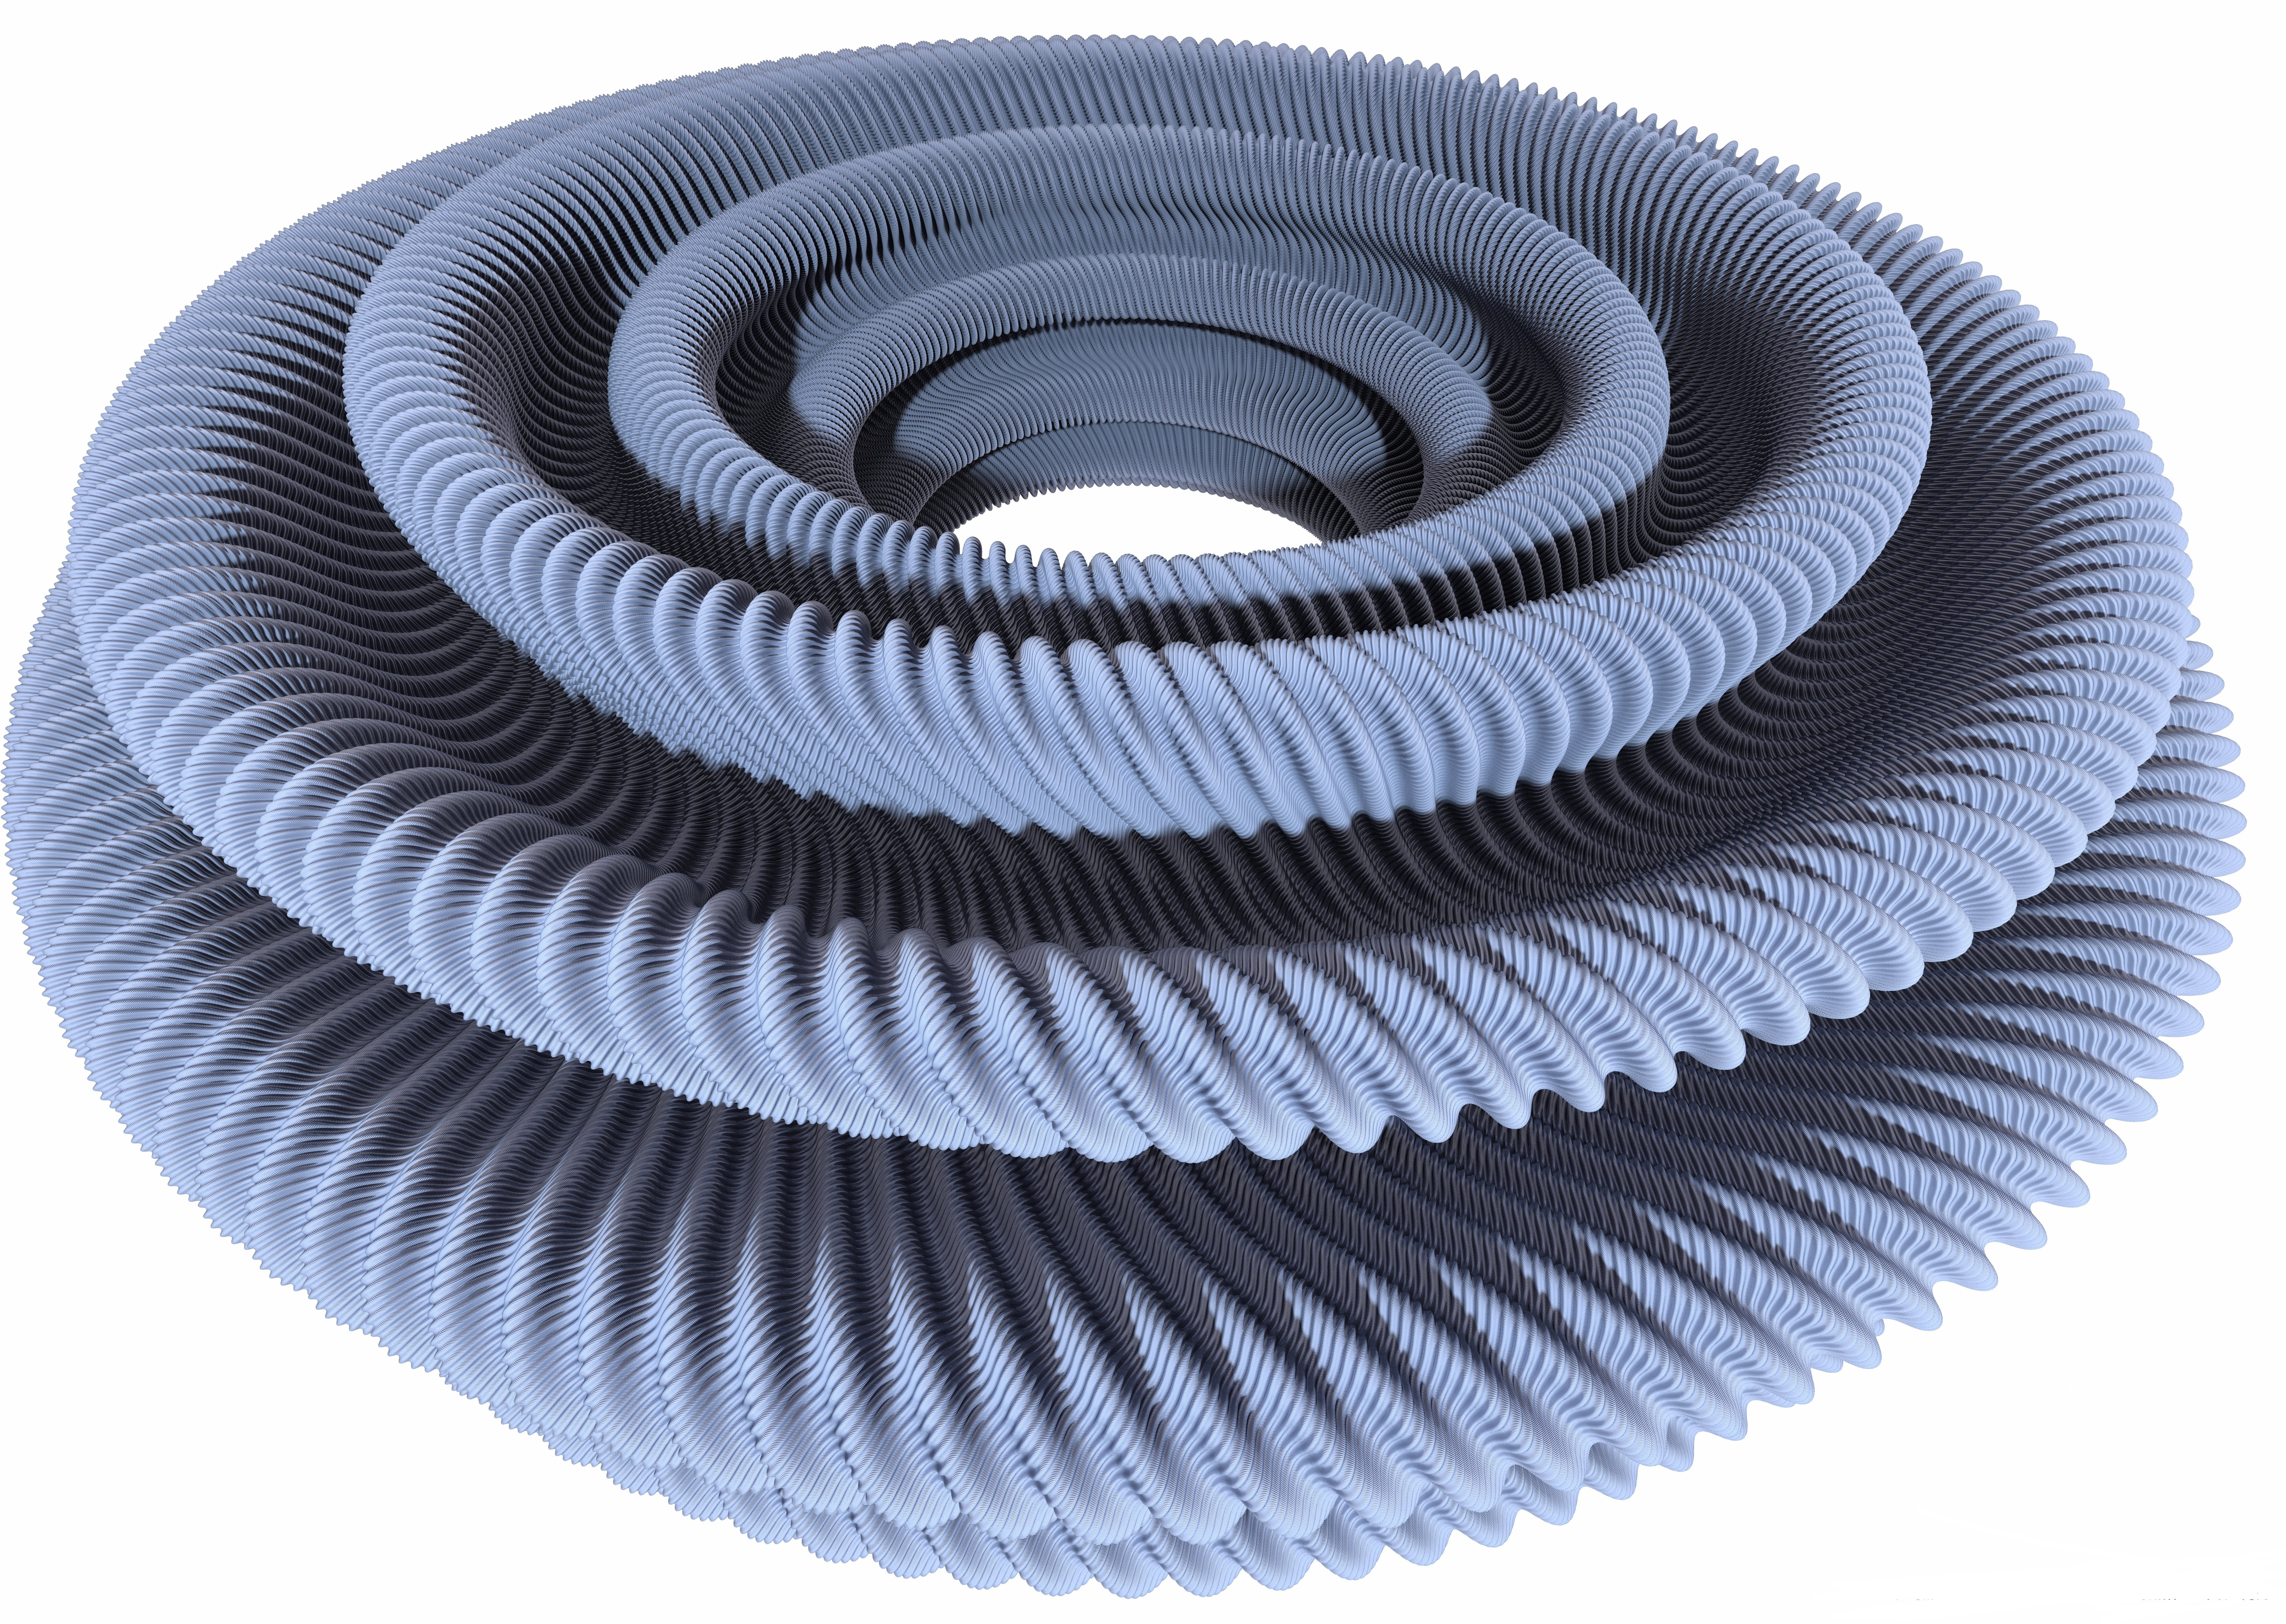
\includegraphics[width=0.5\textwidth]{Tor/tor pla.jpg}
    \caption{Encabiment isomètric del tor pla obtingut amb integració convexa. Figura de \citet{borrelli2013}.}
    \label{fig:tor_pl} 
\end{figure}

Així, aquesta imatge no és només una curiositat matemàtica abstracta, sinó que representa la sorprenent flexibilitat que guanyen els encabiments de varietats riemannianes quan es relaxa la condició de regularitat.

%\chapter{Apunts d'integració convexa}
El que segueix són apunts del seminari \textit{Convex Integration, Staircase Laminates and Applications} d'en Daniel Faraco, de part de la Universitat Autònoma de Madrid, el dia 17 de març de 2025. BGSMATH2025.

\section{Dia 1}
La integració convexa comença amb l'article de Nash sobre les encabiments $C^1$. La pregunta era si pots posar una esfera de manera isomètrica en una esfera més petita. Fiques una varietat $2D$, l'esfera, en una esfera en $\mathbb R^3$. 

La condició \textbf{d'isometria} és que $Du^\intercal Du = g$. Nash comença amb una immersió curta i troba una d'isomètrica. 

Esculls adequadament les pertorbacions de la immersió i obtens el resultat, com ja sabem. El resultat no és particularment útil, potser, però el mètode concret que fa servir és el que anomenem \textbf{integració convexa}, que és molt útil. En general, si hi ha una sèrie de PDE i les dones a través del límit d'unes pertorbacions, donada una subsolució final. 
$$u^\infty = \lim_{N\to\infty} u^N,$$
on $u^{N+1} - u^N = \omega_q$ i $\omega_q$ té paràmetres d'oscil·lació i concentració $\lambda_q$ i $\tau_q$, amb direccions $\eta_k^1\eta_k^2$. i funcions oscil·lants $\phi$.

Considerarem que les aplicacions curtes són \textbf{límits febles}, on els límits febles tals que 
$$\not\int_E u_\gamma \to \not\int_E \overline u$$
FORMULA 1, són \textbf{course grain solutions}. Diu que en aplicacions a PDE, la solució seria \say{micro} i el límit feble seria \say{macro}.

Gromov és potser qui comença a desenvolupar aquest mètode de Nash. Altres van veure que això servia en dinàmica de fluids. 

\textbf{Laminats d'escala} són un mètode inventat pel Faraco per resoldre equacions el·líptiques isotròpiques. Es fan en tres passos:
\begin{itemize}
    \item[(1)] Escriure el problema com una inclusió diferencial: trobar un conjunt $K\subseteq M^{m\times n}$ tal que $u:\Omega\to\mathbb R^m$ i $Du(x)\in K$ a.e. $x\in\Omega$, on $K$ és un conjunt tancat euclidià que representa les dades del problema.
    \item[(2)] Aproximar la solució per $K$ per $$\int\text{dist}_K(Du)^p\le\varepsilon$$.
    \item[(3)] Combinar moltes solucions aproximades per construir una solució exacta.
\end{itemize}
Veurem aquí tota una sèrie d'aplicacions.

\subsubsection{Teoria de Calderón Zygmund}
Tenint en compte aquestes propietats i definició de la transformada de Fourier, FORMULA 2.

Per Plancherel, FORMULA 3, les derivades estan controlades per la laplaciana en la norma $L^2$. Però en $L^1$ això no és cert:
\begin{teo}\label{teo:primer}
    $\forall N,\Omega$ regular $\exists f_N$ amb $\int|\partial_{x1x2}f|\ge N$ i $\sup\set{|\partial_{x1x1}|,|\partial_{x2x2}|}\le 1$
\end{teo}

\subsubsection{Equacions el·líptiques i aplicacions quasiconformals}
En electrostàtica, si $u$ és el potencial elèctric, aleshores 
\begin{itemize}
    \item[--] $\text{div}(\rho\nabla u) = 0$ on $\rho$ la conductivitat.
    \item[--] Condició de frontera $u|_{\partial\Omega} = g$
    \item[--] Quan $\rho = 1$: $\text{div}(\nabla u) = \Delta u$
\end{itemize}
El·lipticitat quantitativa:
$$\frac1KI\le\rho(x)\le KI$$

La solució feble en forma distribucional és $$\int_\Omega\rho\nabla u \nabla \phi \text dx = 0,\quad,\forall\phi\in C_0^\infty(\Omega)$$
La manera d'arribar a això és amb la primera variació del funcional d'energia
$$I[u] = \int_\Omega\rho|\nabla u|^2\text dx$$
Però hem de veure quin és l'espai en què això té sentit. En general, necessitem $W^{1,2}(\Omega)$. La pregunta és si són solucions febles honestes. Hi ha qui les anomena solucions molt febles. 

I ara està parlant de coses del BIMR que no arribo a entendre. 

\section{Dia 2}
Mirarem C-Z en $L^1$, equacions el·líptiques, homeomorfismes patològics etc., on el que ens interessa és que els podem escriure $Df(x)\in E\subseteq M^{m\times n}$. 

El mètode que explicarà sera trobar $Df(x)\in E\subseteq M^{m\times n}$ tal que hi ha un exponent crític $p$ a $(J)$ tal que $Df\in L^{p,\infty}\subset\cap_{q<p}L^q\setminus L^p$.

Pel que fa a CZ ens interessa veure que no és vàlid en $L^1$. És a dir, que exiteis $u$ tal que $\int|\partial_{x1x2}u|=\infty$ però $|\partial_{x1x1}|+|\partial_{x2x2}|\le 1$.

Vam deduir l'operador estrella de Hodge, $\star$, per equacions el·líptiques. Les derivades conformes i anticonformes es poden escriure com coordenades complexes d'una matriu $2\times 2$. 

Si $A = \begin{pmatrix}a_{11}&a_{12}\\a_{21}&a_{22}\end{pmatrix} = (a_-,a_+)$, aleshores $\partial_{\overline z}f = \pm \kappa\overline{\partial_z}f$.
Escrivim $Df \in E_{\pm\kappa} = \set{a_-=\pm\kappa a_+}$. Si tenim una matriu conforme i diagonal, aleshores està en una diagonal. El que tenim ara és en dos plans, $a_-=-\kappa a_+$ i $a_-=\kappa a_+$. MIRAR DIBUIX.

\subsubsection{Beltrami no lineals}
$\partial_{\overline z}f = \mu\partial_z f$, ${\partial_{\overline z}f} = v\overline{\partial_z}f$, $\partial_{\overline z}f =\mu\partial_z f + v\overline{\partial_z}f$
es poden posar en una certa forma.



\section{Dia 3}
Recordem que el que volem, donat $u:\mathbb R^2\to\mathbb R^2$, descriure 
$$Du(x)\in K\quad\textrm{a.e. x}\quad (I)$$
Quina és la integrabilitat de $Du$? 
I volem reformular el problema com:
$$\exists g.d. v_u \text{ tal que } ...$$





\section{Dia 4}
Volem, com sempre, $Du\in K$ tal que $Du\in L^{p,\infty}\setminus L^p$ per algun $p$ crític.
Això és el mateix que fer una distribució de gradients tq el suport de $v_u\in K$, $v_u(x:|x|\ge t)\approx t^{-p}$.
Que serà el mateix que construir un laminat d'escala tal que $v_u\in\mathcal{SL}^p(K)$ 

Recordem que diem que $A$ i $B$ són rang 1 connectades si $A-B=a\otimes n$ tal que $\det(A-B)=0$. Per tant, $\forall 0\le\lambda\le1$, $\lambda s_A+(1-\lambda)s_B$ és (aprox) distribució de gradients.

Amb això podem trobar ua funció amb distribució de gradients només un en $A$ i un en $B$ (l'espai gradient vius a l'espai de les matrius, generat per $(1 0, 0 0)$ i $(0 0, 0 1)$ ) Aleshores les direccions de rang 1 són les horitzontals i verticals. El centre de masses d'una mesura generada (en horitzontal) per A i B està en el segment entre $A$ i $B$.

Les propietats que té la distribució de gradients per tal que funcionin és que siguin afins a trossos amb condicions afins de frontera, que ens fa més fàcil generar laminats. Si tenim $ABABAB$ haurem de posar a la frontera lateral una regió d'interpolació, i no hi ha problema canviant per exemple $B$ per $DEDEDE$ o alguna cosa així. Cada vegada que fem aquest procés, que la massa de $A$ es divideix entre $B$ i $C$ i la de $B$ entre $D$ i $E$, tenim una altra distribució gradient. 
Ara bé, amb això només podem fer coses amb matrius connectades rang 1. Ara bé, si no són connectades rang 1 això no funciona. El que hem construit fins ara eren prelaminats, els laminats són els límits de successions de prelaminats a mesura que fem més i més petites les cantonades.

La gran contribució de Tartar és que ser un camp gradient és només que el rotacional sigui 0. Anul·lar el rotacional és com resoldre un sistema d'equacions de primer ordre, per exemple $\mathcal L(z) = A_{ijk}\partial_j z^k$. Per cada operador diferencial existeix el que anomenem con d'ones $\Lambda_L$, el subconjunt de $\mathbb R^n$ tal que si $I\in\Lambda_L$ aleshores exiteix una direcció $\xi$ tal que per qualsevol $h:\mathbb R\to \mathbb R$ tenim que $\mathcal L(h)$ LHA TRET :(, que generalitza el concepte de connexió de rang 1.

Aquesta teoria no es restringeix només a gradients, sinó també a coses de Fraday blablabla.

Definició de laminat escala: tenim un conjunt $K\in M^{d\times m}$ on vull que es suporti, i $A\not\in K$. Aleshores l'esglaó $n$ serà $\omega_1=(1-\gamma_n)\mu_n+\gamma_n\delta_{A_n}$ i tal, de manera que anem pujant i suportant-nos on toca.











\newpage
\section{Apunts del paper de Nash del 1954}
{
\color{blue}
\begin{itemize}
    \item Parlar abans de la diferència entre el punt de vista extrínsec i intrínsec de la geometria, un cop haguem parlat de geodif. 
    \item Veurem que una varietat de dimensió $n$ es pot ficar en un espai $E^{2n}$, on aquí diem que $E^k$ és l'espai euclidià de dimensió $k$.
    \item Interessant que el procés de les correccions sempre augmenta les distàncies localment, motiu pel qual el primer ha de ser curt. Diu Nash que l'anem "estirant".
    \item Mirar el tema de si la caracterització de una immersió curta és diferent que a la que dona SJO.
    \item Si la varietat és tancada només cal canviar l'escala de $E^k$ per fer la immersió curta. Si és oberta cal fer una cosa més complicada.
    \item Coses a tenir en compte:
        \begin{itemize}
            \item $g_{ij}$ és la mètrica intrínseca, $h_{ij}$ és la mètrica induïda.
            \item $\set{x^i}$ són les coordenades en la varietat $M$.
            \item $\set{z^\alpha}$ són les coordenades en $E^k$.
            \item Amb la immersió, $z^\alpha = z^\alpha(x^1, \dots, x^n)$.
            \item La mètrica induïda és $h_{ij} = \frac{\partial z^\alpha}{\partial x^i}\frac{\partial z^\beta}{\partial x^j}$. Normalment estaria multiplicat per una $g_{\alpha\beta}$ que no apareix perquè en aquest cas és la mètrica euclidiana.
        \end{itemize}
    \item Cada correcció es va fent en infinites "etapes", cada una d'elles corregint la correcció de la etapa anterior. L'important aquí és que cada correcció manté el fet que la immersió sigui curta, tot i que cada vegada menys. Cada etapa ens hi hauria d'apropar la meitat del camí. Per exemple, després de la primera, l'error hauria de ser
    $$g_{ij}-\overline{h_{ij}}\approx \frac12(g_{ij}-h_{ij})$$
    \item Ho fem d'aquesta manera perquè així ens assegurem que cada correcció només ha d'augmentar la mètrica. 
    \item Cada etapa es divideix en passes (passos?), que afecten només localment la immersió augmentant la mètrica en una sola direcció. 
    \item Per tal de dividir en passos, dividim la varietat en una sèrie d'entorns amb $n$ paràmetres $C^\infty$ no singulars, i cada entorn es pot trobar amb un nombre finit d'altres entorns.
    \item Per cada un d'aquests entorns, per exemple $N_p$, prenem una funció $\varphi_p$ positiva a l'interior de $N_p$ i $0$ fora d'ell. Definim aquestes funcions tals que la suma de totes les $\varphi_p$ valgui $1$ en qualsevol punt. (Això com es fa? Diu que és estàndard però em sembla una mica complicat si ha de ser $C^\infty$.) Això serveix per distribuir la "càrrega" de la correcció.
    \item En cada entorn, la "càrrega" de la correcció es divideix també entre les passes. Sigui $\delta_{ij}=g_{ij}-h_{ij}$ l'error mètric després d'unes quantes etapes. A la propera voldríem augmentar la mètrica més o menys $\frac12\delta_{ij}$, de manera que a l'entorn $N_p$ voldríem augmentar la mètrica en $\frac12\varphi_p\delta_{ij}$. Per fer-ho haurem de trobar un tensor definit positiu $\beta_{ij}$ que sigui $C^\infty$ i aproximi $\delta_{ij}$.
    \item $$\frac12\varphi_p\beta_{ij} = \sum_{\nu}a_{\nu}\frac{\partial\psi^\nu}{\partial x^i}\frac{\partial\psi^\nu}{\partial x^j}$$ on $x^i$ són coordenades de l'entorn $N_p$, $a_\nu$ funcions no-negatives $C^\infty$ i $\psi^\nu$ funcions lineals en $x^i$.
    \item A l'apartat \textbf{The normal fields}, diu que necessita dos camps vectorials unitaris $C^\infty$ normals a la immersió i ortogonals entre ells, $\zeta^\alpha$ i $\eta^\alpha$. Això és lo de la co-dimensió 2 que després Kuiper canvia a 1.
    \item La pertorbació associada a $a_\nu$ i $\psi^\nu$ és 
        \begin{equation}
            \boxed{\overline{z}^\alpha = z^\alpha + \zeta^\alpha\frac{\sqrt{a_\nu}}{\lambda}\cos(\lambda \psi^\nu) + \eta^\alpha\frac{\sqrt{a_\nu}}{\lambda}\sin(\lambda \psi^\nu)}
        \end{equation}
        on $\lambda$ és un paràmetre que podem triar.
    \item El canvi mètric és $\sum_\alpha\frac{\partial\overline{z}^\alpha}{\partial x^i}\frac{\partial\overline{z}^\alpha}{\partial x^j}-\sum_\alpha\frac{\partial z^\alpha}{\partial x^i}\frac{\partial z^\alpha}{\partial x^j}$. No cal calcular tots els termes en detall, perquè molts contenen $1/\lambda$ o $1/\lambda^2$ i, per tant, convergeixen uniformement a $0$ quan $\lambda\to\infty$. Altres termes es cancel·len. CALDRIA FER AIXÒ A MÀ.
    \item $\lambda$ no fa desaparèixer els termes en què s'ha derivat les trigonomètriques, perquè en surt una $\lambda$ de dins. Ara bé, ens queden termes de l'estil $\sum_\alpha\frac{\partial z^\alpha}{\partial x^i}\zeta^\alpha\sqrt{a_\nu}(-\sin(\lambda \psi^\nu))\frac{\partial\psi^\nu}{\partial x^j}$, o amb les $i$ i $j$ bescanviades o amb $\eta^\alpha$ en comptes del $\zeta^\alpha$. Cadascun d'aquests termes són $0$, ja que $\zeta$ i $\eta$ són normals a la immersió.
    \item La resta de termes tindran el producte de dues funcions trigonomètriques o el quadrat d'una d'elles. Les que tinguin el producte també contenen $\zeta^\alpha\eta^\alpha$, i desapareixen per ortogonalitat.
    \item El que queda, doncs és 
    $$\sum_\alpha (\zeta^\alpha)^2 a_\nu (\sin^2(\lambda \psi^\nu) ) \frac{\partial\psi^\nu}{\partial x^i}\frac{\partial\psi^\nu}{\partial x^j} + \sum_\alpha (\eta^\alpha)^2 a_\nu (\cos^2(\lambda \psi^\nu) ) \frac{\partial\psi^\nu}{\partial x^i}\frac{\partial\psi^\nu}{\partial x^j}$$
    i si traiem factor comú i usem que els vectors són unitaris, ens queda
    $$a_\nu\frac{\partial\psi^\nu}{\partial x^i}\frac{\partial\psi^\nu}{\partial x^j}$$
    que és el que volíem.
    \item I amb això veiem que l'error mètric és $O(1/\lambda)$.
    \item A \textbf{Size of immersion...} repetim que la pertorbació canvia segons $O(1/\lambda)$ després de cada passa. Mirant el que fa a la primera derivada, veiem el canvi que fa en un entorn totes les passes d'una etapa, i queda que el canvi en les derivades acaba sent $$\left|\left( \frac{\partial z^\alpha}{\partial x^i}\right)_{\text{final}}-\left( \frac{\partial z^\alpha}{\partial x^i}\right)_{\text{inicial}}\right| \le 2\sqrt{K\beta_{ii}}+O(1/\lambda_1)+\dots + O(1/\lambda_\nu)+\cdots$$ LA VERITAT ÉS QUE NO SÉ D'ON SURTEN ELS TRES PUNTS DEL FINAL.
    \item A \textbf{Global considerations and convergence} volem veure quina $\lambda$ s'ha d'agafar. 
    \begin{itemize}
        \item[$\bullet$] $B_1$ és el màxim error que volem en l'aproximació del canvi mètric, \\$a_\nu\left(\frac{\partial\psi^\nu}{\partial x^i}\right)\left(\frac{\partial\psi^\nu}{\partial x^j}\right)$.
        \item[$\bullet$] $B_2$ és el màxim error $O(1/\lambda)$ que volem en el canvi de les primeres derivades.
        \item[$\bullet$] $B_3$ és la cota de $\overline{z}^\alpha - z^\alpha$.
    \end{itemize}
    \item Després d'una etapa, la nova mètrica induïda és $h'_{ij} = h_{ij} + \frac12\delta_{ij}$. Posem $h'_{ij} = g_{ij} - \delta'_{ij}$, on $\delta'_{ij} =-\frac12\delta_{ij} +e_{ij}$ i $e_{ij}$ és un terme d'error. Per tal que la successió convergeixi, necessitem que $\delta'_{ij}$ sigui estrictament més petita que $\delta_{ij}$. Si imposem que en tot punt de $N_p$ el màxim dels components de $e_{ij}$ sigui menor o igual a un sisè del màxim de $\delta_{ij}$, aleshores el màxim de $\delta'_{ij}$ serà menor o igual a dos terços del màxim de $\delta_{ij}$. MIRAR SI AIXÒ ÉS ALGUNA NORMA $C^k$ O ALGO.
    \item Volem que $\delta'_{ij}$ sigui definida positiva, que ho podem assegurar si imposem que la mida de $e_{ij}$ sigui més petita que un cert $\varepsilon_p$ que depèn de l'entorn compacte $N_p$. Com cada entorn se superposa amb un nombre finit $\sigma$ d'altres entorns, es poden trobar límits per $e_{ij}$ tal que el que busquem sigui cert en tots ells. Anomenem $\varepsilon_p^*$ el mínim d'aquestes limitacions.  
    \item L'error ve de l'aproximació de $\delta_{ij}$ per $\beta_{ij}$ i dels passos. Per tant, imposant $(\delta_{ij}- \beta_{ij}) < \varepsilon_p^*$, tenim que $(\frac12\varphi_p\delta_{ij}- \frac12\varphi_p\beta_{ij}) < \frac12\varepsilon_p^*$. Així, podem imposar que en un entorn $N_p$ els passos tinguin aquesta seqüència de $B_{1}$: $B_{11}\le\frac14\varepsilon_p^*$, $B_{12}\le\frac18\varepsilon_p^*$, $B_{13}\le\frac1{16}\varepsilon_p^*$, etc.
    \item A \textbf{Performability of the steps} simplement diu que a cada pas tenim una immersió $C^\infty$ i que tot és definit positiu. La única font de negativitat és l'error, però això sempre es pot contenir amb $\lambda$.
    \item A \textbf{General organization} es fa aquest resum:
        \begin{itemize}
            \item[$\bullet$] El procés es fa en una sèrie d'etapes que prenen una immersió curta $C^\infty$ i en retornen una amb un error mètric com a molt $2/3$ del de l'anterior.
            \item[$\bullet$] La varietat es divideix en entorns $N_p$. 
            \item[$\bullet$] Cada etapa es divideix en passos. A cada etapa, la correcció és pesada per $\varphi_p$ i dividida per tal que la duguin a terme les passes. 
            \item[$\bullet$] Si la varietat és oberta, hi ha un nombre infinit de passos per etapa, però a cada porció compacta hi ha un nombre finit.
        \end{itemize}
    \item A \textbf{Convergence of the immersion} diu que necessitem que les $B_3$ del pas $r$ de l'etapa $s$ siguin més petites que $2^{-(r+s)}$, i el mateix per $B_2$. La manera per fer-ho és escollir que la mida de $\beta_{ij}$ estigui entre $9/10$ i $9/8$ de la de $\delta_{ij}$. Això fa que el canvi en les derivades estigui limitat per una geomètrica de raó $\sqrt{5/6}$ MIRAR AIXÒ, de manera que les funcions $C^\infty$ convergeixen uniformement a una de $C^1$.
    \item ES MOLT IMPORTANT QUE ESCRIVIM ALGUNA COSA SOBRE LA DIFERÈNCIA ENTRE IMMERSIONS I encabiments.
    \item A \textbf{Isometric Imbeddings} {\color{black!50!green} QUAN PARLA DE CONJUNT LÍMIT CREC QUE ES REFEREIX A LA PART DEL CONJUNT OBERT MÉS LLUNYANA, EL QUE ESTARIA JUST A TOCAR DE LA FRONTERA} diu que per encabiments és bàsicament el mateix, però necessitem controlar les auto-interseccions. Per veure que pas a pas no n'hi ha, cal comprovar que per $\lambda$ prou gran les evitem. 
    \item Sigui $M$ un conjunt tancat de l'encabiment que conté $N_p$ al seu interior. $M$ té un entorn obert $H$ tal que no hi ha punt de $H$ amb dues rectes perpendiculars a $M$. MIRAR AIXÒ, HI HA UNA CITA.
    \item Posem $Q$ la unió del conjunt límit amb la part de la encabiment que no està a l'interior de $M$. Aleshores $Q$ és tancat i una pertorbació prou petita de $N_p^*$ no afectarà $Q$. AQUÍ NO SÉ QUÈ ÉS $N_p^*$. EN GENERAL, AQUEST APARTAT ES POSA MOLT TÈRBOL. 
    \item A \textbf{Constructing the initial immersion} explica que si la varietat té dimensió $n$, sabem que es pot trobar una encabiment en $E^{2n}$ no-singular i analítica. Es pot prendre aquesta immersió i escalar-la per a que sigui curta. 
    \item Per un conjunt obert, podem recobrir la varietat per entorns $N_p$ pesats amb funcions $C^\infty$ $\varphi_p$ amb paràmetres $x_{pi}$ tals que $|x_{pi}|\le1$. Volem que en qualsevol punt de la varietat els conjunts d'aquest recobriment se superposin un nombre finit de vegades $s$, com a molt.
    \item Podem dividir els conjunts $N_p$ en $s$ classes, de manera que en cada classe no hi hagi conjunts que es superposin. 
    \item Podem definir una encabiment en un espai $s(n+2)$ dimensional, a partir de funcions $u_\sigma=\varepsilon_p\varphi_p$ en conjunts de la classe $\sigma$ i $0$ en la resta, $v_\sigma=\varepsilon^2_p\varphi_p$ en conjunts de la classe $\sigma$ i $0$ en la resta, i $w_\sigma=\varepsilon_p\varphi_px_{pi}$ en conjunts de la classe $\sigma$ i $0$ en la resta, on $x_{pi}$ la coordenada $i$-èssima de $N_p$ i $\set{\varepsilon_p}_p$ és una successió monòtona decreixent de nombres positius que convergeix a $0$.
    \item Observem: que totes aquestes funcions són $C^\infty$, que dos punts de conjunts interiors a conjunts diferents tenen raons $v_\sigma/u_\sigma$ diferents, i que punts interiors a un mateix entorn $N_p$ tenen $w_{\sigma i}$ diferents. (EL CONJUNT LÍMIT ÉS L'ORIGEN PERÒ CAP PUNT ÉS ENVIAT A L'ORIGEN)
    \item Podem escollir que la encabiment sigui curta escollint la successió $\set{\varepsilon_p}_p$. Si la mètrica induïda pels primers $p$ entorns és curta per un factor $\frac13(2-1/p)$, podem escollor $p+1$ tal que sigui curta per un factor $1/3(2-1/(p+1))$. Amb això tenim una encabiment curta i $C^\infty$ en $E^{s(n+2)}$, i a partir de projeccions podem arribar a $E^{2n+1}$
    \item A \textbf{General summary} enumera els quatre teoremes que ha demostrat en aquest article:
    \begin{itemize}
        \item[$\bullet$] \begin{teo}
            Qualsevol varietat riemanniana tancada de dimensió $n$ té una encabiment isomètrica $C^1$ en $E^{2n}$.
        \end{teo}
        \item[$\bullet$] \begin{teo}
            Qualsevol varietat riemanniana de dimensió $n$ té una immersió isomètrica $C^1$ en $E^{2n}$ i una encabiment isomètrica $C^1$ en $E^{2n+1}$.
        \end{teo}
        \item[$\bullet$] \begin{teo}
            Si una varietat riemanniana tancada de dimensió $n$ té una immersió o encabiment $C^\infty$ en $E^{k}$ amb $k\ge n+2$, aleshores també té una immersió o encabiment, respectivament, isomètrica en $E^{k}$.
        \end{teo}
        \item[$\bullet$] \begin{teo}
            Si una varietat riemanniana oberta de dimensió $n$ té una immersió o encabiment $C^\infty$ curta en $E^{k}$ amb $k\ge n+2$ que no se solapa amb el seu conjunt límit (si aquest existeix), aleshores també té una immersió o encabiment, respectivament, isomètrica en $E^{k}$ del mateix tipus.
        \end{teo}
    \end{itemize}
    \item Per últim, un comentari super interessant que fa és que potser es pot canviar $n+2$ per $n+1$ si es fa una una pertorbació diferent que només necessita una direcció, que crec que és just el que fa Kuiper!
\end{itemize}

}









\begin{equation}\label{eq:un_mig_de_phi_p}
    \frac12\varphi_p\beta_{ij} = \sum_{\nu}a_{\nu}\frac{\partial\psi^\nu}{\partial x^i}\frac{\partial\psi^\nu}{\partial x^j}
\end{equation}
\begin{lema}
    L'equació \eqref{eq:un_mig_de_phi_p} es pot satisfer amb les condicions necessàries.
\end{lema}
{\color{black!50!green}\textit{Prova.} Les matrius simètriques definides positives formen un con de dimensió $\frac12n(n+1)$.{\color{blue} D'on surt això? És molt estrany} És possible cobrir aquest con amb conjunts simplicials {\color{blue} MIRAR A WIKIPEDIA EL QUE ÉS} geomètrics oberts, de tal manera que cada punt del con estigui cobert per, com a molt, un nombre $W$ d'aquests entorns, on $W$ depèn només de $n$. 

Una matriu qualsevol representada per un punt d'un símplex és combinació lineal de les matrius que representen els vèrtexs del símplex. Podem posar
$$\begin{aligned}
    &C_{1,1}; \quad C_{1,2}; \quad C_{1,3}; \quad \dots\\
    &C_{2,1}; \quad C_{2,2}; \quad C_{2,3}; \quad \dots\\
    &\vdots\\
    &C_{q,1}; \quad C_{q,2}; \quad C_{q,3}; \quad \dots
\end{aligned}$$
els coeficients per $q$ representacions d'una matriu del con.
Ara podem escriure uns altres coeficients
$$ C_{\mu,\nu}^* = \frac{C_{\mu,\nu} \exp\set{-\sum_\sigma 1/C_{\mu,\sigma}}}{\sum_{\rho}\exp\set{-\sum_\sigma 1/C_{\rho,\sigma}}}, $$
de manera que aquests coeficients són $C^\infty$ com a funcions de la matriu que representen. Per cada matriu, com a molt $W[\frac12n(n+1)+1]$ coeficients $C_{\mu,\nu}^*$ són no-nuls.

Si ara considerem que $\beta_{ij}$ defineix una aplicació $C^\infty$ de $N_p$ al con, aleshores podem escriure 
\begin{equation}
    \beta_{ij} = \sum_{\mu,\nu}C_{\mu,\nu}^*M_{(\mu,\nu)ij}
\end{equation}
on $M_{(\mu,\nu)ij}$ són les diferents matrius que representen els vèrtexs dels símplexs. Ara, per cada matriu $M_{(\mu,\nu)ij}$ obtenim $n$ autovectors unitaris ortogonals $\set{V_r}$ i els seus autovalors $\set{v_r}$.

Si $\psi_r$ és per cada $r$ la funció lineal dels paràmetres locals pels quals $\sqrt{v_r}V_r$ és el vector gradient {\color{blue}Aquesta és la part més rara, entenc que simplement es pot fer}, tenim que
\begin{equation}
    M_{(\mu,\nu)ij} = \sum_{r}\frac{\partial\psi_r}{\partial x^i}\frac{\partial\psi_r}{\partial x^j}
\end{equation}
i, substituint en \eqref{eq:beta_con}, tenim que
\begin{equation}
    \beta_{ij} = \sum_{r}\sum_{\mu,\nu}C_{\mu,\nu}^*M_{(\mu,\nu)ij}\frac{\partial\psi_r}{\partial x^i}\frac{\partial\psi_r}{\partial x^j}
\end{equation}
i, agrupant termes en $a_\nu$, obtenim el resultat.\qed
}




























\newpage
\section{Explicació del Sung-Jin Oh}
\begin{teo}\label{teo: SJO} Sigui $(M,g)$ una superfície, $N\ge\dim M+1$ i $u:M\to\mathbb R^N$ una encabiment estrictament curta, és a dir, tal que la longitud de cada vector en $M$ s'escurça (estrictament) sota $\nabla u$. Aleshores $u$ es pot aproximar uniformement per encabiments isomètriques $C^1$.
\end{teo}
{\color{blue} Haurem d'explicar què és una encabiment isomètrica, i mirar si cal que li canviem el nom}

Per exemple, l'homotècia $\mathbb S^2\to\varepsilon\mathbb S^2$ amb $\varepsilon\in(0,1)$ és una aplicació \textit{curta}. 
\begin{obs}
De fet, qualsevol encabiment $C^2$ isomètrica $u:\mathbb S^2\hookrightarrow\mathbb R^3$ ha de ser igual a la encabiment estàndard $\mathbb S^2 \hookrightarrow\set{ x\in\mathbb R^3 : |X| = 1 }$ fins translació i rotació. 
\end{obs}

El teorema \ref{teo: SJO} es demostra amb \textit{integració convexa}.

Sung-Jin Oh demostra aquí el Baby Nash theorem.


Sigui $D=\set{x\in\mathbb R^2 : |x|<1}$ el disc unitat, i $g = g_{ij}(x)$ una mètrica de $D$. Una aplicació $u:D\to\mathbb R^n$ és una \textit{immersió} {\color{blue} per ara direm encabiment als embeddings i immersions als \textit{immersions}} si $\nabla u(x)$ és injectiva per tot $x$. La mètrica en $D$ induïda per $u$ és de la forma {\color{blue} Haurem de recordar i controlar el que era la mètrica induïda}
\begin{equation*}
    \nabla u ^{\intercal}(x)\nabla u (x) = \begin{pmatrix}
    \nabla_1 u\nabla_1 u & \nabla_1 u\nabla_2 u\\
    \nabla_2 u\nabla_1 u & \nabla_2 u\nabla_2 u
    \end{pmatrix}
\end{equation*}
Diem que l'aplicació és \textit{isomètrica} {\color{blue} també estaria bé comentar isometries} si $\nabla u ^{\intercal}\nabla u = g$, i diem que és \textit{(estrictament) curta} si $\nabla u(x)^{\intercal} \nabla u(x) - g(x) \le 0$ per tot $x\in D$.
\begin{teo}\label{Baby Nash} [Baby Nash]
    Sigui $n\ge 4$ i $u:D\to\mathbb R^n$ una immersió estrictament curta. Per qualsevol $\varepsilon > 0$, existeix una immersió isomètrica $C^1$ $\tilde u:D\to\mathbb R^n$ tal que $\|u-\tilde u\|_{C^0(D)} < \varepsilon$.{\color{blue} Aquí cal motivar l'interès d'aquest resultat. Entenc que la idea és que partim d'una immersió que és estrictament curta i volem trobar una que sigui contínua i isomètrica. Vull mirar continuïtats.}
\end{teo}
\begin{obs}
    Aquest teorema necessita que la co-dimensió sigui com a mínim 2.
\end{obs}
La manera de demostrar aquest resultat és a través d'un mètode iteratiu amb passos altament oscil·lants.
Sigui $u_1 = u + U$ amb 
\begin{equation*}
    U=\sum_{I\in\mathcal I} U_I
\end{equation*}
Volem que cada component $U_I^j$ sigui complex, per tal que oscil·li com $e^{ix \cdot \xi}$, però que el resultat del sumatori sigui real. Així, imposem que per cada $I\in\mathcal I$ que existeixi $\overline I\in\mathcal I$ tal que 
\begin{equation*}
    U_{\overline{I}} = \overline{U}_I, \quad \overline{\overline{I}} = I.
\end{equation*}
Ara tenim un error mètric $h_1 = g - \nabla u_1 ^{\intercal}\nabla u_1$. {\color{blue} On entenem que l'error mètric és la diferència entre la mètrica i la mètrica induïda per la immersió? Té sentit, però cal veure per què només agafo el primer terme.}
\begin{equation*}
    h_1 = 
        \left( h-\sum_{I} \nabla \overline{U}_I ^{\intercal}\nabla U_I \right) 
        - \sum_{I}\left( \nabla u ^{\intercal}\nabla U_I + \nabla U_I ^{\intercal}\nabla u \right)
        - \sum_{I,J: J\not = \overline I} \nabla U_I ^{\intercal}\nabla U_J.
\end{equation*}
I anomenem els tres sumands, en ordre, $q_{\text{mèt}}$, $q_{\text{lin}}$ i $q_{\text{alt}}$.

Volem una correcció que oscil·li en una sola direcció $\xi\in\mathbb R^2$, $|\xi|=1$. Posem
\begin{equation*}
    U_I = W = \frac1\lambda a(x)\textbf{n}(x)e^{\lambda i x \cdot \xi},
\end{equation*}
amb $a:D\to\mathbb R$ i $\textbf{n}:D\to\mathbb C^n$ tal que $\textbf{n}\cdot \overline{\textbf{n}}=1$. Per tal que sigui real, definim també $\overline I\in\mathcal I$ tal que 
\begin{equation*}
    U_{\overline{I}} = \overline W = \frac1\lambda a(x)\overline{\textbf{n}}(x)e^{-\lambda i x \cdot \xi}.
\end{equation*}

Per eliminar el terme $q_{\text{mèt}}$, observem que
\begin{equation*}
    \begin{aligned}
    \nabla_j W &= i\xi_j a(x)\textbf{n}(x)e^{\lambda i x \cdot \xi} + \frac{1}{\lambda}\nabla_j (a(x)\textbf{n}(x))e^{\lambda i x \cdot \xi}\\
    &=i\xi_j a(x)\textbf{n}(x)e^{\lambda i x \cdot \xi} + O(\frac{1}{\lambda})
    \end{aligned}
\end{equation*}
{\color{blue} EXPLICAR PER QUÈ ÉS O(1/LAMBDA)!!! De fet, explicar d'on surt la lambda aquesta.}
I, per tant,
\begin{equation*}
    \begin{aligned}
    \nabla_i W^*(x) \nabla_jW(x)&= (-i\xi_ia(x)e^{-\lambda i x \cdot \xi})(i\xi_ja(x)e^{\lambda i x \cdot \xi})\overline{\textbf{n}}(x) \cdot\textbf{n}(x) + O(\frac{1}{\lambda})\\
    &= \xi_i\xi_j a(x)^2 + O(\frac{1}{\lambda})
    \end{aligned}
\end{equation*}
on definim $(\cdot)^* = (\overline{\cdot})^\intercal$. Així, l'oscil·lació és cancel·lada i en resulta un terme $a(x)^2\xi_i\xi_j$.
\begin{ex}
    {\color{blue} EXPLICAR MILLOR AQUEST EXEMPLE}
    Posem que per un cert $x\in D$, l'error $h$ és de la forma
    \begin{equation*}
        h(x) = a^2(x)\xi \otimes \xi + b^2(x)\xi' \otimes \xi' + c^2(x)\xi'' \otimes \xi''
    \end{equation*}
    aleshores, amb això fem desaparèixer el terme $\xi \otimes \xi$. Repetint-ho per $\xi' \otimes \xi'$ i $\xi'' \otimes \xi''$ aconseguim reduir l'error $h(x)$ a un terme $O(\frac{1}{\lambda})$.
\end{ex}
\begin{obs}
    {\color{blue} EXPLICAR AQUESTA OBSERVACIÓ}
    Aquest mètode requereix que $h$ sigui curta, ja que $\nabla_i W^*(x) \nabla_jW(x)$ és un terme no-negatiu. De fet, per tal que $h_1$ sigui curt, necessitem que $h$ sigui estrictament curt.
\end{obs}
Ara bé, els autovectors $\xi$ depenen d'$x$. Això es pot resoldre amb el següent lema.
\begin{lema}\label{lema:descomposicio_error_metric} (Descomposició de l'error mètric)
    Sigui $\mathcal P$ l'espai de totes les matrius definides positives. Existeix una successió $\xi^{(k)}$ de vectors unitaris en $\mathbb R^n$ i una successió $\Gamma_{(k)}\in C_c^\infty(\mathcal P; [0,\infty))$ tals que
    \begin{equation*}
        A_{ij} = \sum_k\Gamma^2_{k}(A)\xi_i^{(k)}\xi_j^{(k)}
    \end{equation*}
    i aquesta suma és \textit{localment finita}. És a dir, existeix $N\in\mathbb N$ tal que per tot $A\in\mathcal P$ com a màxim $N$ termes de $\Gamma_{(k)}$ són no-nuls.
\end{lema}
\begin{obs}
    La demostració d'aquest teorema no l'escrivim aquí explícitament. {\color{blue} ESTÀ AL SUNG-JIN OH.}
\end{obs}
Fins ara no ha calgut especificar el vector $\textbf{n}(x)\in\mathbb C^n$ per tal de minimitzar l'error mètric, més enllà que necessitem que sigui unitari. Veurem que el podem escollir de tal manera que els termes $q_{\text{lin}}$ i $q_{\text{alt}}$ desapareguin fins a terme $O(1/\lambda)$.
\begin{itemize}

    \item \textbf{Error de linearització.} Substituïm el terme amb $W$
    \begin{equation*}
         \nabla_i u ^{\intercal}\nabla_j W = i\xi_j a(x)e^{ix\cdot\xi}\nabla_i u\cdot\textbf{n}+O(1/\lambda)
    \end{equation*}
    i veiem que podem eliminar aquest component escollint un vector perpendicular a l'espai tangent de $u(x)$, $\textbf{n}(x)\perp \nabla_j u(x)$. Això es pot fer perquè l'espai té co-dimensió 1 ({\color{blue}REVISAR!!!}). Podem fer el mateix amb $\nabla_iW^{\intercal}\nabla_ju$ i obtenim
    \begin{equation*}
        \nabla_i u ^{\intercal}\nabla_j W + \nabla_iW^{\intercal}\nabla_ju = O(1/\lambda)
    \end{equation*}

    \item \textbf{Interferència altament oscil·lant.} De nou, substituïm el terme
    \begin{equation*}
        \nabla_iW^{\intercal}\nabla_jW = (-a^2(x)\xi_i\xi_je^{2ix\cdot\xi})\textbf{n}\cdot\textbf{n} + O(1/\lambda).
    \end{equation*}
    I ara només cal utilitzar que la encabiment té co-dimensió $\ge2$ per escollir un vector complex tal que $\textbf{n}\cdot\textbf{n} = 0$ {\color{blue}Com està definit aquest producte?}. Podem prendre, per exemple, 
    \begin{equation*}
        \textbf{n} = \frac{1}{i\sqrt2}\zeta(x) + \frac{1}{\sqrt2}\eta(x)
    \end{equation*}
    on $\zeta(x)$ i $\eta(x)$ són vectors reals unitaris ortogonals a l'espai tangent $T_{u(x)}u(D)$.
    \item \textbf{Forma final de la correcció.} Tot plegat, tenim una correcció de la forma
    \begin{equation*}
        W(x) = \frac{a(x)}{\lambda}\left( \sin(\lambda x \cdot \xi)\zeta(x) + \cos(\lambda x \cdot \xi)\eta(x) \right)
    \end{equation*}
    amb les següents propietats:
    \begin{itemize}
        \item[--] Norma $C^0$ petita {\color{blue} Explicar C-normes}: $$||W||_{C^0}\le C\frac{||a||_{C^0}}{\lambda}$$
        \item[--] Terme principal en $\nabla W$ 
        \begin{equation*}
            \begin{aligned}
                \nabla W = &a(x)\left( \cos(\lambda x \cdot \xi)\zeta(x) - \sin(\lambda x \cdot \xi)\eta(x) \right) \\
                &+ O_{||a||_{C^0}, ||\nabla a||_{C^0}, ||\nabla\zeta||_{C^0}, ||\nabla\eta||_{C^0}}(1/\lambda)
            \end{aligned}
        \end{equation*}
        \item[--] Error mètric petit: $$\nabla_i W^{\intercal}\nabla_j W(x) -a^2(x)\xi_i\xi_j = O(1/\lambda)$$
        \item[--] Error de linearització petit: $$\nabla_i u ^{\intercal}\nabla_j W + \nabla_iW^{\intercal}\nabla_ju = O(1/\lambda)$$
        \item[--] Error d'interferència petita: $$\nabla_i W ^{\intercal}\nabla_j W = O(1/\lambda)$$
    \end{itemize}
\end{itemize}
\begin{obs}
    {\color{blue} Aquesta derivada es pot entendre si l'escrius i fas els passos. Mirar si cal explicar-ho millor.}
    Una manera alternativa d'arribar a la forma general de la correcció és la següent. Definim 
    \begin{equation*}
        \begin{aligned}
        \gamma = (\gamma_1, \gamma_2) : &D\times \mathbb T\to \mathbb R^2\\
        & (x,t)\mapsto \gamma(x,t)
        \end{aligned}
    \end{equation*}
    on $\mathbb T = \mathbb R / 2\pi\mathbb Z$.
    Posant $\dot\gamma$ la derivada respecte de $t$, tenim que
    \begin{equation*}
        \nabla W ^{\intercal}(x) \nabla W(x) = \left( \dot\gamma_1^2(x, \lambda x\cdot\xi) + \dot\gamma_2^2(x, \lambda x\cdot\xi) \right)\xi\otimes\xi + O(1/\lambda).
    \end{equation*}
    De manera que per cada $x$ cal trobar $\gamma(x,\cdot)$ tal que 
    (1) $\dot\gamma_1^2 + \dot\gamma_2^2 = a^2$ i 
    (2) $t\mapsto \dot\gamma(x,t)$ sigui $2\pi$-periòdic i $\int\dot\gamma\text{d}t = 0$
    De manera que $t\mapsto\gamma(x,t)$ també ha de ser $2\pi$-periòdica i el seu origen ha de pertànyer al disc unitat tancat $\overline D$.
    {\color{blue} IMPORTANT Per a després, NASH ANOMENA STEP A CADA ADDICIÓ D'UNA CORRECCIÓ, que es carrega un terme a un error d'ordre $O(1/\lambda)$. }
\end{obs}
\begin{lema}[Lema d'iteració]\label{Lema_iteracio}
    Sigui $u:D\to\mathbb R^n$ una immersió suau estrictament curta, tal que $h:=g-\nabla u ^{\intercal}\nabla u$ obeeix
    \begin{equation}
        ||h||_{C^0} \le e_h
    \end{equation}
    per algun $e_h > 0$. Aleshores, per qualsevol $\varepsilon > 0$, existeix una immersió suau estrictament curta $u_{[1]} = u + U$, on
    \begin{equation}
        \begin{aligned}
        ||U||_{C^0(D)} &\le \varepsilon\\
        ||\nabla U||_{C^0(D)} &\le Ce_h^{1/2}
        \end{aligned}
    \end{equation}
    i $h_{[1]}:=g-\nabla u_{[1]}^{\intercal}\nabla u_{[1]}$ obeeix
    \begin{equation}
        ||h_{[1]}-h||_{C^0} \le \varepsilon.
    \end{equation}
\end{lema}
\textit{Prova.} Pel lema \ref{lema:descomposicio_error_metric}, tenim que $h$ es pot escriure com
\begin{equation*}
    h(x) = \sum_k \Gamma^2_{(k)}(h(x))\xi^{(k)}\otimes\xi^{(k)}
\end{equation*}
on per cada $h(x)$ hi ha com a molt $K$ termes no-nuls.

Per la compacitat d' $h(D)\subseteq\mathcal P$, existeix un nombre finit de sumands que són funcions no-nul·les{\color{blue} Non-vanishing, mirar la traducció}. Reanomenem aquests sumands d'aquesta manera:
\begin{equation*}
    \Gamma^2_{(1)}(h(x))\xi^{(1)}\otimes\xi^{(1)}, \Gamma^2_{(2)}(h(x))\xi^{(2)}\otimes\xi^{(2)}, \dots, \Gamma^2_{(N)}(h(x))\xi^{(N)}\otimes\xi^{(N)}
\end{equation*}
Prenent la traça, veiem que 
\begin{equation*}
    ||\Gamma_{(j)}(h)||_{C^0} \le ||h||_{C^0}^{1/2} \le e_h^{1/2}
\end{equation*}
{\color{blue} Mirar d'on surt això (Sembla Cauchy-Schwarz, però què passa amb la traça de h?)}
Ara podem fer $N$ correccions a $u$ de la mateixa manera que hem fet abans, en les direccions $\xi^{(1)}, \xi^{(2)}, \dots, \xi^{(N)}$, per cancel·lar aquests errors. En concret, per un $\delta>0$, definim de manera recursiva $u_j = u_{j-1}+(1-\delta)^{1/2}U_j$, amb $u_0 = u$ i 
\begin{equation*}
    U_j = \frac{\Gamma_{(j)}(h(x))}{\lambda_j}\left( \sin(\lambda_j x\cdot\xi^{(j)})\zeta_j(x) + \cos(\lambda_j x\cdot\xi^{(j)})\eta_j(x) \right)
\end{equation*}
per uns certs $\lambda_j$ i $\zeta_j, \eta_j:D\to\mathbb R^n$ unitaris.

Prenem $\delta > 0$ per tal d'assegurar curtedat estricta {\color{blue} no sé com es diu shortness la veritat}. De fet, fixem $0<\delta<\frac{\varepsilon}{2e_h^{1/2}}$ per tal que $h\ge\delta I$. {\color{blue} uiuiui això mirar-ho bé}

Escollint $\lambda_j$ prou gran, tenim
\begin{itemize}
    \item[--]
    \begin{equation}
        ||U_j||_{C^0} \ll \varepsilon
    \end{equation}
    \item[--]
    \begin{equation}
        \nabla U_j = \Gamma_{(j)}(h)\xi^{(j)}(\cos(\lambda_j x\cdot\xi^{(j)})\zeta - \sin(\lambda_j x\cdot\xi^{(j)})\eta) + \text{err}_j,\quad ||\text{err}_j||_{C^0} \ll \varepsilon
    \end{equation}
    \item[--]
    \begin{equation}
        h_j=h_{j-1}-(1-\delta)\Gamma^2_{(k)}(h)\xi^{(j)}\xi^{(j)} + \text{err}_j', \quad ||\text{err}_j'||_{C^0} \ll \delta^2
    \end{equation}
    {\color{blue} Les dues primeres són fàcils d'entendre, però la tercera l'hem de revisar.}
\end{itemize}
On $h_j=g-\nabla u_j ^{\intercal}\nabla u_j$. 

Per tal de concloure la prova, verifiquem que $U=U_1+\dots+U_N$ i $u_{[1]}=u_N=u+U$ satisfan les propietats desitjades.

\begin{itemize}
    \item És fàcil veure que $||U_j|| \ll \varepsilon$ implica $||U||_{C^0(D)} \ll \varepsilon$.
    \item A més, de $\nabla U_j = \Gamma_{(j)}(h)\xi^{(j)}(\cos(\lambda_j x\cdot\xi^{(j)})\zeta - \sin(\lambda_j x\cdot\xi^{(j)})\eta) + \text{err}_j$ i $||\Gamma_{(j)}(h)||_{C^0} \le e_h^{1/2}$ tenim que $||\nabla U||_{C^0(D)} \le Ke_h^{1/2} + \sum_{j=1}^N ||\text{err}_j||_{C^0} \le 2Ke_h^{1/2}$ si es prenen les constants adequades. 
    \item Finalment, sumant els termes $h_j$ obtenim 
    \begin{equation*}
        h_N = h-(1-\delta)\sum_{j=1}^N \Gamma^2_{(j)}(h)\xi^{(j)}\xi^{(j)} + \sum_{j=1}^N \text{err}'_j = \delta h + \sum_{j=1}^N \text{err}'_j
    \end{equation*}
    i imposant que $u_{[1]} = u_N$ sigui estrictament curta, $h_{[1]}=h_N \ge \delta^2 I$, obtenim el resultat.
\end{itemize}
\qed

Ara podem iterar diverses vegades per concloure la prova del teorema \ref{Baby Nash}.

\textit{Prova del teorema \ref{Baby Nash}.} Sigui $e_{h,[k]}>0$ una successió tal que
$$\sum_{k}e_{h,[k]}\le \epsilon,\quad\sum_{k}e_{h,[k]}^{1/2}<\infty.$$ 
Pel lema \ref{Lema_iteracio}, obtenim una successió d'aplicacions suaus estrictament curtes $u_{[k]}$ tal que $u_{[0]}=u$ i
\begin{equation*}
    \begin{aligned}
    ||g-\nabla u_{[k]}^\intercal\nabla u_{[k]}||_{C^0} &\le e_{h,[k]}\\
    ||\nabla u_{[k+1]}-\nabla u_{[k]}||_{C^0} &\le Ce^{1/2}_{h,[k]}\\
    ||u_{[k+1]}-u_{[k]}||_{C^0} &\le e_{h,[k+1]},
    \end{aligned}
\end{equation*}
demostrant el teorema.\qed

{\color{blue} revisar això últim perquè just estava parlant amb la marina}
\subsection{Extensions}
\subsubsection{Extensió a encabiments de varietats}
Per estendre el teorema \ref{Baby Nash} a immersions a superfícies generals, només cal reduir a cartes coordenades. Per estendre'l a encabiments usem que, per la compacitat d'$M$, podem trobar $\varepsilon>0$ tal que 
$$\inf_{x,y} \text{dist}(u(x), u(y))\ge\varepsilon.$$ Ara només cal dur a terme la construcció en un entorn de $0.01\varepsilon$.{\color{blue} entendre millor això últim perquè és bastant random}
\subsubsection{Refinament de Kuiper: encabiment de codimensió 1}
Modificant la forma de la correcció, podem aconseguir la mateixa construcció amb només co-dimensió 1. Sigui $\eta:D\to\mathbb R^{3}$ el camp vectorial unitari en $u(D)$, i sigui
$$\zeta = \nabla u (\nabla u^\intercal \nabla u)^{-1}\xi.$$
Prenem 
$$U = \frac1\lambda \left( \gamma_{1}(x, \lambda x \cdot \xi)\tilde{\zeta}(x) + \gamma_{2}(x, \lambda x \cdot \xi)\tilde{\eta}(x) \right)$$
on 
$$\tilde{\zeta} = \frac{\zeta}{|\zeta|^2}, \quad \tilde{\eta} = \frac{\eta}{|\zeta|},$$
i $u_1 = u + U$. Això porta a 
{\color{blue} paper i boli}
$$\nabla u_1^\intercal \nabla u_1 = \nabla u^\intercal \nabla u +\frac{1}{|\zeta|^2}\left( 2\dot\gamma_{1} + \dot\gamma_1^2 + \dot\gamma_{2}^2 \right) \xi \otimes \xi + O(1/\lambda).$$
De manera que per cada $x$ i $a=a(x)\in\mathbb R$ volem que $\gamma$ sigui tal que
\begin{itemize}
    \item {\color{blue} posar això amb la cosa aquella de (1) i (2)}
    \item $(1+\dot\gamma_1)^2+\dot\gamma_2^2=|\zeta|^2a^2+1$,
    \item $t \mapsto \dot\gamma(x,t)$ és $2\pi$-periòdica i $\int\dot\gamma\textrm{d}t=0$
\end{itemize}
i tal que $|\dot\gamma|\le C|a|$. Això és possible perquè l'envolupant convexa de $\set{(x,y):(1+x)^2+y^2 = |\zeta|^2a^2+1}$ conté el $0$. 




\newpage
\section{Varietats topològiques}
\begin{defi} 
    Sigui $M$ un espai topològic. Diem que $M$ és una \textbf{varietat topològica de dimensió $n$} si es compleixen les propietats següents:
    \begin{itemize}
        \item $M$ és \underline{Hausdorff}, és a dir, si per a cada $p,q\in M$ amb $p\neq q$ existeixen entorns oberts $U\subseteq M$ i $V\subseteq M$ de $p$ i $q$ respectivament tals que $U\cap V = \emptyset$,
        \item $M$ verifica el \underline{segon axioma de numerabilitat}, és a dir, existeix una base numerable de la topologia de $M$,
        \item $M$ és \underline{localment homeomorf a $\mathbb R^n$}, és a dir, per a cada $p\in M$ existeix un entorn obert $U\subseteq M$ de $p$ que és homeomorf a un obert de $\mathbb R^n$.
    \end{itemize}
\end{defi}
{\color{blue} Es pot posar un exemple}

Per tal de poder descriure localment els punts de les varietats i de poder operar amb ells, serà útil introduir el concepte de carta coordenada.

\begin{defi}
    Sigui $M$ una varietat topològica de dimensió $n$. Diem que un parell $(U,\varphi)$ és una \textbf{carta coordenada de $M$} si $U$ és un obert de $M$ i $\varphi:U\to\hat U$ és un homeomorfisme amb un obert $\hat U\subseteq\mathbb R^n$. Anomenem $U$ el \textbf{domini de la carta} i $\varphi$ la \textbf{funció coordenada}.
\end{defi}
\begin{obs}
    De la definició de carta coordenada, observem que no tota varietat topològica $M$ es pot cobrir amb una única carta coordenada. Per exemple, si $M$ és homeomorf al cercle $\mathbb S^1$ amb la topologia induïda per $\mathbb R^2$, no es pot trobar cap aplicació $\varphi:M\to\mathbb R$ que sigui un homeomorfisme amb un obert de $\mathbb R$, ja que $\mathbb S^1$ és compacte.
\end{obs}

{\color{blue} Es pot posar un exemple.}

A continuació, donarem algunes propietats de les varietats topològiques i les cartes coordenades, sense reproduir les demostracions explícitament.

\begin{lema}
    Tota varietat topològica es pot recobrir amb numerables cartes coordenades.
\end{lema}


\begin{lema}
    Tota varietat topològica té una base numerable de boles coordenades amb adherència compacta.
\end{lema}


\begin{prop}
Sigui $M$ una varietat topològica. Aleshores, 
\end{prop}
{
    \begin{itemize}
        \item \textit{$M$ és localment arc-connexa.}{\color{blue} Aquí utilitzo arc-connexa com a sinònim de connex per camins.}
        \item \textit{$M$ és connex si i només si és arc-connex.}
        \item \textit{Els components connexos de $M$ són els seus components arc-connexos.}
        \item \textit{$M$ té un conjunt numerable de components connexos, i cada un d'ells és un obert i una varietat topològica connexa.}
    \end{itemize}
}
\begin{prop}
    Tota varietat topològica és localment compacta. És a dir, per a cada $p\in M$ existeix un entorn obert $U$ de $p$ tal que $U\subseteq K$ per algun compacte $K\subseteq M$.
\end{prop}
\begin{defi}
    Diem que una col·lecció $\mathcal X$ de subconjunts d'un espai topològic $M$ és \textbf{localment finita} si per a cada $p\in M$ existeix un entorn obert $U$ de $p$ tal que $U\cap X = \emptyset$ per a tots $X\in\mathcal X$ excepte un nombre finit d'ells.
\end{defi}
\begin{defi}
    Donat un recobriment per oberts $\mathcal U$ d'un espai topològic $M$, diem que un recobriment per oberts $\mathcal V$ és un \textbf{subrecobriment de $\mathcal U$} si per a cada $V\in\mathcal V$ existeix $U\in\mathcal U$ tal que $V\subseteq U$.
\end{defi}
\begin{defi}
    Diem que un espai topològic $M$ és \textbf{paracompacte} si qualsevol recobriment per oberts de $M$ té un subrecobriment localment finit.
\end{defi}
\begin{teo}
    Tota varietat topològica és paracompacta. De fet, donat un recobriment per oberts $\mathcal X$ i qualsevol base $\mathcal B$ de la topologia de $M$, existeix un subrecobriment numerable localment finit $\mathcal V$ de $\mathcal X$ format només d'elements de $\mathcal B$.
\end{teo}
{\color{blue} Aquesta demostració està en el Lee, no té gaire a veure amb el tema així que potser no la posem, però bueno, allà està.}
\section{Estructura suau}













\newpage
\section{Suavitat}
{\color{blue} L'Ignasi m'ha dit que el que hauria de ressaltar més és la diferència entre $C^1$ i $C^\infty$. Potser podria comentar alguns dels resultats que són vàlids en un i no en l'altre?}
{\color{blue} El que hi ha aquí ho estic traient de wikipedia. Preguntar a l'Ignasi per una font més bona.}
\begin{defi}
    Sigui $U\subseteq\mathbb R$ un conjunt obert, $f:U\to\mathbb R$ una funció real contínua.
    Diem que $f$ és {\normalfont $k$-vegades derivable contínuament}, amb $k\in\mathbb N_0$, si la derivada d'ordre $k$, $$f^{(k)}:= \frac{d^k}{dx^k}f,$$ existeix i és contínua en $U$. Anomenem l'índex $k$ \textit{suavitat} de $f$.
    Diem que $f$ és {\normalfont suau} o {\normalfont infinitament derivable} si existeix la derivada de qualsevol ordre.
\end{defi}
\begin{obss}
\end{obss}
\begin{itemize}
    \item $f$ és $0$ vegades derivable contínuament si i només si $f$ és contínua. 
    \item Si $f$ és $k$ vegades derivable contínuament, aleshores també és $j$ vegades derivable contínuament per $0\le j\le k$.
\end{itemize}
\begin{defi}
    Anomenem \textit{classe de diferenciabilitat} $C^k(U)$, amb $k\in\mathbb N_0$ l'espai de les funcions $k$-vegades derivables contínuament en $U\subseteq\mathbb R^n$. Anomenem $C^\infty(U)$ l'espai de les funcions infinitament derivables en $U$.
\end{defi}
De la mateixa manera, podem definir aquests conceptes per funcions de diverses variables.
\begin{defi}
    Sigui $U\subseteq\mathbb R^n$ un conjunt obert, $f:U\to\mathbb R$ una funció real contínua.
    Diem que $f$ és \textit{$k$-vegades derivable contínuament}, amb $k\in\mathbb N_0$, si totes les seves derivades parcials d'ordre $k$, $$\frac{\partial^k}{\partial x_1^{\alpha_1}\cdots\partial x_n^{\alpha_n}}f,$$ tals que $\sum_{i=1}^n\alpha_i = k$, existeixen i són contínues en $U$. És a dir, si $f$ és $k$-vegades derivable contínuament en cada component de $U$.
\end{defi}
\begin{defi}
    Anomenem \textit{classe de diferenciabilitat} $C^k(U)$, amb $k\in\mathbb N_0$ l'espai de les funcions $k$-vegades derivables contínuament en $U\subseteq\mathbb R^n$. Anomenem $C^\infty(U)$ l'espai de les funcions infinitament derivables en $U$.
\end{defi}
\begin{obss}{\color{blue} Potser caldria donar la definició explícita en el cas de funcions de diverses variables.}
\end{obss}
\begin{itemize}
    \item Moltes vegades, en lloc de $C^k(U)$ es fa servir $C^k(U;\mathbb R^m)$ per a funcions $f:U\to\mathbb R^m$.
    \item També escriurem simplement $C^k$ en lloc de $C^k(U)$ si el domini és clar pel context.
\end{itemize}

\subsection{Classes de diferenciabilitat com espais normats}
A continuació definirem normes en $C^k(U)$ i $C^\infty(U)$ que ens permetran tractar-les com espais vectorials normats.
\begin{defi}
    Sigui $U\subseteq\mathbb R^n$ un conjunt obert, $f:U\to\mathbb R^m$ una funció. Definim la norma $\|\cdot\|_{C^k(U)}$ de $f$ com
    \begin{equation*}
        \|f\|_{C^k(U)} = \sum_{|\alpha|\le k} \|D^\alpha f\|_{L^\infty(U)},
    \end{equation*}
    on $\|\cdot\|_{L^\infty(U)}$ és la norma del suprem en $U$, tal que $\|g\|_{L^\infty(U)} = \sup_{x\in U} |g(x)|$.
\end{defi}
{\color{blue} Aquí podríem proposar i demostrar que $\|\cdot\|_{C^k(U)}$ és efectivament una norma, ho tenim a \url{https://proofwiki.org/wiki/C%5Ek_Norm_is_Norm}. També cal decidir si definim explícitament la $D^\alpha$.}

\section{Fonaments de geometria diferencial}
Aquí hauriem de parlar d'embedding preferiblement.






\newpage
\section{Temes de les reunions}
Sigui $\mathcal M$ una varietat diferenciable amb una distància $d$, i sigui $$\nu = \set{(x,v)\in \mathcal M \times \mathbb R^n: v\in T_x\mathcal M^{\perp}}.$$ Per qualsevol $\varepsilon > 0$, definim el subconjunt $$\nu_\varepsilon = \set{(x,v)\in \nu: ||v|| < \varepsilon}$$
i l'aplicació $$\begin{aligned}
    \sigma:\nu_\varepsilon &\to \mathbb R^n \\
    (x,v) &\mapsto x+v
\end{aligned}$$
\begin{teo}
    Si $\varepsilon$ és prou petit, aleshores $\sigma:\nu_\varepsilon \to \sigma(\nu_\varepsilon)$ és homeomorfisme.
\end{teo}
{\color{black!50!green}\textit{Prova. (Meva, està molt millor al John M. Lee)} Primer, volem veure que $\sigma$ és injectiva. Suposem que $\mathcal M$ és $C^\infty$ (amb $C^2$ hauria de ser prou). Donat qualsevol punt $x\in\mathcal M$ existeix un entorn prou petit $U_x$ de $x$ en $\mathcal M$ tal que $\nu_1$ és injectiva. Això és degut al fet que, localment, la varietat és aproximadament igual al seu espai tangent. 

Sigui $x_0$ el punt amb l'entorn $U_{x_0}$ més petit que verifica la propietat anterior, i sigui $y_0$ el punt de $\mathcal M\setminus U_{x_0}$ tal amb el vector $w_0\in T_{y_0}\mathcal M$ més curt tal que existeix algun $v_0\in T_{x_0}\mathcal M$ tal que $x_0+v_0=y_0+w_0$. 
Sigui $l=||w_0||$. Aleshores, posant $\varepsilon = l/2$, tenim que $\sigma$ és injectiva. 

Pel que fa a la exhaustivitat, $\sigma:\nu_\varepsilon \to \sigma(\nu_\varepsilon)$ és exhaustiva per definició. A més, en ser la suma de dos vectors en $\mathbb R^n$, $\sigma$ és contínua.

Cal veure que la inversa $\sigma^{-1}$ és contínua. Sigui $a\in \sigma(\nu_\varepsilon)$. Aleshores, existeixen $x\in \mathcal M$ i $v\in \mathbb R^n$ tals que $a=\sigma(x,v)=x+v$. Com $\sigma^{-1}$ projecta punts de $\sigma(\nu_\varepsilon)$ en el punt de $\nu_\varepsilon$ més proper, tenim que $\sigma^{-1}$ és contínua.
Per tant, $\sigma$ és un homeomorfisme. \qed}
\begin{obs} 
    D'aquí surt el que fa servir Nash per allò del conjunt que no admet dues perpendiculars.
\end{obs}
\newpage

% \chapter{Conclusions}

% Hem après un muntHI HA UNA EXPLICACIó DE COM CITAR AL CAMPUS

\normalfont

\newpage
\bibliographystyle{unsrt}
\begin{thebibliography}{25}

% { \color{blue} \bibitem[Autor1 \& Autor2(ANY)]{nomdelacita}
% Autor1, A., \& Autor2, B. (ANY)
% \newblock \textit{Nom del treball.}
% \newblock Cambridge University Press.
% }
\bibitem[Nash(1954)]{nash1954}
Nash, J. (1954)
\newblock \textit{$C^1$ isometric imbeddings.}
\newblock Annals of Mathematics, 60(3), 383-396.

\bibitem[Kuiper(1955)]{kuiper1955}
Kuiper, N. H. (1955)
\newblock \textit{On $C^1$-isometric imbeddings. I}
\newblock Indagationes Mathematicae(Proceedings), 58, 545-556.

\bibitem[Schwartz(2024)]{schwartz2024}
Schwartz, R. E. (2024)
\newblock \textit{The Optimal Paper Moebius Band.}
\newblock arXiv:2308.12641

\bibitem[Borrelli et al.(2013)]{borrelli2013}
Borrelli, V., Jabrane, S., Lazarus, F., \& Thibert, B. (2013)
\newblock \textit{Isometric embeddings of the square flat torus in ambient space.}
\newblock Ensaios Matemáticos (Sociedade Brasileira de Matemática), 24, 1-98.

\bibitem[Cartan(1927)]{cartan1927}
Cartan, E. (1927)
\newblock \textit{Sur la possibilité de plonger un espace riemannien donné dans un espace euclidien.}
\newblock Ann. Soc. Pol. Math., 6, 1-7.

\bibitem[Rokhlin(1970)]{rokhlin1970}
Gromov, M. i Rokhlin, V. (1970)
\newblock \textit{Embeddings and immersions in riemannian geometry.}
\newblock Russian Math. Survey, 5, 1-57.

\bibitem[Lee(2013)]{lee2013}
Lee, J. M. (2013)
\newblock \textit{Introduction to smooth manifolds.}
\newblock Springer.

\bibitem[Warner(1983)]{warner1983}
Warner, F. W. (1983)
\newblock \textit{Foundations of differentiable manifolds and Lie groups.}
\newblock Springer.

\bibitem[Chavel(2006)]{chavel2006}
Chavel, I. (2006)
\newblock \textit{riemannian geometry: A modern introduction.}
\newblock Cambridge University Press.

\bibitem[Oh(2018)]{oh2018}
Oh, S. J. (2018)
\newblock \textit{The Nash $C^1$ isometric embedding theorem.}
\newblock [Apunts d'una xerrada].





\end{thebibliography}
\end{document} 

